%===============================================================================
% LaTeX sjabloon voor de bachelorproef toegepaste informatica aan HOGENT
% Meer info op https://github.com/HoGentTIN/latex-hogent-report
%===============================================================================

\documentclass[dutch,dit,thesis]{hogentreport}

\usepackage{lipsum} % For blind text, can be removed after adding actual content

%% Pictures to include in the text can be put in the graphics/ folder
\graphicspath{{graphics/}}

%% For source code highlighting, requires pygments to be installed
%% Compile with the -shell-escape flag!
\usepackage[section]{minted}
\usemintedstyle{solarized-light}
\definecolor{bg}{RGB}{253,246,227} %% Set the background color of the codeframe

%% Change this line to edit the line numbering style:
\renewcommand{\theFancyVerbLine}{\ttfamily\scriptsize\arabic{FancyVerbLine}}

%% Macro definition to load external java source files with \javacode{filename}:
\newmintedfile[javacode]{java}{
    bgcolor=bg,
    fontfamily=tt,
    linenos=true,
    numberblanklines=true,
    numbersep=5pt,
    gobble=0,
    framesep=2mm,
    funcnamehighlighting=true,
    tabsize=4,
    obeytabs=false,
    breaklines=true,
    mathescape=false
    samepage=false,
    showspaces=false,
    showtabs =false,
    texcl=false,
}

% Other packages not already included can be imported here

%%---------- Document metadata -------------------------------------------------
\author{Nicolas Thiers}
\supervisor{Dhr. B. Vertonghen}
\cosupervisor{Dhr. M. Vandeperre}
\title%[subtitel]%
    {Het performantie verschil tussen een REST API en een gRPC API bij het versturen van datasets}
\academicyear{\advance\year by -1 \the\year--\advance\year by 1 \the\year}
\examperiod{1}
\degreesought{\IfLanguageName{dutch}{Professionele bachelor in de toegepaste informatica}{Bachelor of applied computer science}}
\partialthesis{false} %% To display 'in partial fulfilment'
%\institution{Internshipcompany BVBA.}

%% Add global exceptions to the hyphenation here
\hyphenation{back-slash}

%% The bibliography (style and settings are  found in hogentthesis.cls)
\addbibresource{bachproef.bib}            %% Bibliography file
\addbibresource{../voorstel/voorstel.bib} %% Bibliography research proposal
\defbibheading{bibempty}{}

%% Prevent empty pages for right-handed chapter starts in twoside mode
\renewcommand{\cleardoublepage}{\clearpage}

\renewcommand{\arraystretch}{1.2}

%% Content starts here.
\begin{document}

%---------- Front matter -------------------------------------------------------

\frontmatter

\hypersetup{pageanchor=false} %% Disable page numbering references
%% Render a Dutch outer title page if the main language is English
\IfLanguageName{english}{%
    %% If necessary, information can be changed here
    \degreesought{Professionele Bachelor toegepaste informatica}%
    \begin{otherlanguage}{dutch}%
       \maketitle%
    \end{otherlanguage}%
}{}

%% Generates title page content
\maketitle
\hypersetup{pageanchor=true}

%%=============================================================================
%% Voorwoord
%%=============================================================================

\chapter*{\IfLanguageName{dutch}{Woord vooraf}{Preface}}%
\label{ch:voorwoord}

Tijdens mijn opleiding Toegepaste Informatica met afstudeerrichting Mobile \& Enterprise developer heb ik verschillende REST API's moeten ontwikkelen
waardoor deze standaard daarmee de meest voor de hand liggende keuze is bij het opstarten van een kersverse applicatie. Vaak zonder voldoende alternatieven te overwegen.
Tegelijkertijd werden we er tijdens de opleiding toch voldoende bewust van gemaakt dat er nog andere mogelijkheden en technologie\"en beschikbaar zijn waarbij o.a. gRPC naar boven gekomen is.
De kans om hier meer kennis over te vergaren en praktische ervaring en mijn nieuwsgierigheid hebben mij voor dit onderwerp doen kiezen.\\

Van de gelegenheid maak ik gebruik om mijn co-promotor, Maarten Vandeperre, te bedanken. Zeker bij het opzetten en deployen van de server applicatie was
zijn kennis en ervaring een enorme hulp. Ook bij het bepalen van de manier van testen is zijn feedback zeer waardevol geweest.\\

Graag wens ik ook mijn promotor, Benjamin Vertonghen, te bedanken voor zijn feedback bij de verschillende stadia van het tot stand komen van deze bachelorproef.\\

Tot slot wens ik mijn familie te bedanken voor het vele geduld en de steun tijdens de jaren van deze opleiding. De combinatie van een voltijdse job, een bacheloropleiding en
een gezin was allerminst evident, maar ik besef dat deze opleiding een meerwaarde vormt en ben blij dat ik heb doorgezet.\\

Ik wens u veel leesplezier!
%%=============================================================================
%% Samenvatting
%%=============================================================================

% TODO: De "abstract" of samenvatting is een kernachtige (~ 1 blz. voor een
% thesis) synthese van het document.
%
% Een goede abstract biedt een kernachtig antwoord op volgende vragen:
%
% 1. Waarover gaat de bachelorproef?
% 2. Waarom heb je er over geschreven?
% 3. Hoe heb je het onderzoek uitgevoerd?
% 4. Wat waren de resultaten? Wat blijkt uit je onderzoek?
% 5. Wat betekenen je resultaten? Wat is de relevantie voor het werkveld?
%
% Daarom bestaat een abstract uit volgende componenten:
%
% - inleiding + kaderen thema
% - probleemstelling
% - (centrale) onderzoeksvraag
% - onderzoeksdoelstelling
% - methodologie
% - resultaten (beperk tot de belangrijkste, relevant voor de onderzoeksvraag)
% - conclusies, aanbevelingen, beperkingen
%
% LET OP! Een samenvatting is GEEN voorwoord!

\IfLanguageName{english}{%
\selectlanguage{dutch}
\chapter*{Samenvatting}

\selectlanguage{english}
}{}

%%---------- Samenvatting -----------------------------------------------------
% De samenvatting in de hoofdtaal van het document

\chapter*{\IfLanguageName{dutch}{Samenvatting}{Abstract}}
In dit onderzoek wordt het performantieverschil tussen een REST API en een gRPC API beschouwd bij het versturen van datasets van vari\"erende grootte.
Beide technologie\"en zijn API's en daarmee helpen zij de communicatie tussen twee applicaties via HTTP te faciliteren. gRPC is een tamelijk recente ontwikkeling die
dankzij een speciaal serialisatie- en compressie proces zeer performant zou moeten zijn. De vraag rijst dan in welke mate het sneller zou zijn dan REST en is het dat
in alle omstandigheden.\\
Wanneer de verschillen tussen de beide API's bekeken worden, lopen enkele aspecten extra in de kijker.
Zo kan bij REST nog steeds het HTTP 1.1 protocol gebruikt worden, t.o.v. gRPC dat enkel via het performantere HTTP 2 communiceert.
gRPC gebruikt echter specifieke delen van het HTTP 2 protocol waar moderne browsers geen ondersteuning voor bieden
waardoor voor dergelijke communicatie een extra proxy moet voorzien worden.
gRPC serialiseert en comprimeert alle data d.m.v. protocol buffers waardoor het, op vlak van performantie, een overwicht zou verkrijgen t.a.v. REST.
Bij REST wordt data voornamelijk als JSON verzonden, wat meer uitvoerig is dan de geserialiseerde data via gRPC.
Er is echter geen verplichting voor een specifiek formaat waardoor bij REST data eventueel ook gecomprimeerd kan worden.
Er bestaat zelfs een specifieke Header die aangeeft van welk compressiealgoritme gebruikt moet worden.
In tegenstelling tot gRPC is het gebruik van REST wijdverspreid en zijn er voldoende softwareontwikkelaars met kennis ter zake om een REST API vlot te implementeren.
Voor beide API's is het nodig een betrouwbaar en duidelijk contract aan te bieden aan een eventuele client.
Voor REST zijn er reeds veel oplossingen die een API documenteren en eventueel zelfs code genereren.
Bij gRP dient er een .proto bestand uitgewisseld te worden tussen server en client waarmee de nodige code door protocol buffers gegenereerd kan worden.
Over hoe de uitwisseling van dit bestand best dient te verlopen, lijkt nog geen consensus te zijn gevonden.\\
Elke softwareontwikkelaar of applicatie-architect dient bij de implementatie van een applicatie te evalueren wat de concrete noodzaken
zijn en te overwegen welke technologie\"en daar het beste een oplossing voor bieden. Deze overweging kan enkel gemaakt worden met kennis van zaken. Performantie is
steeds een belangrijk en vaak een doorslaggevende factor.
Het onderwerp van deze scriptie, wat het effectieve performantie verschil is tussen een REST API en een gRPC API voor
datasets van variërende grootte, kan een deel van de puzzel aanbrengen. Zeker aangevuld met de vergelijkende studie in de stand van zaken in dit onderzoek.\\
Voor het onderzoek worden 2 applicaties, client en provider, in Java programmeertaal geschreven, met behulp van het Quarkus framework.
Beide applicaties krijgen 2 rest implementaties, één dat data als JSON verzendt en het andere data met behulp van gzip zal comprimeren alvorens te verzenden.
Ook zijn er 2 gRPC implementaties, het eerste zal de te verzenden data met protocol buffers serialiseren en daarna verzenden en het tweede,
ten volle gebruik makend van HTTP 2 functionaliteit, geeft de geserialiseerde data middels een stream door.
De server applicatie zal gehost worden op OpenShift van RedHat terwijl de client applicatie deze vanop een pc aanspreekt.
Tijdens de performantie-testen wordt het tijdsverloop geregistreerd bij aanvang van het aanroepen van de server door de client
tot de gevraagde data bij de client toekomt en gedeserialiseerd is. Dit proces wordt voor verschillende datasets herhaald.
Ook worden grotere datasets in stukken verzonden om het verschil in performantie te beschouwen.\\
De resultaten geven antwoord op de onderzoeksvraag door aan te tonen dat een standaard REST API, met de opzet gegeven in de methodologie,
tot 3,5 keer trager is dan een standaard gRPC API. Maar wanneer er echter gecomprimeerde data verzonden wordt via het REST API, blijft dit ongeveer even performant te zijn als gRPC.
Via gRPC een stream doorgeven blijkt ook geen heil te bieden met deze opzet.
De bedenking wordt ten slotte gemaakt dat REST een volwassen technologie is die zeer veel gebruikt en algemeen gekend is terwijl gRPC in verhouding een nog tamelijk recente ontwikkeling is.
REST wordt, zelfs bij het verzenden van gecomprimeerde data, ondersteund door nagenoeg alle browsers.
Tot slot wordt vastgesteld dat er nog vragen onbeantwoord blijven omtrent het delen van het .proto bestand.

%---------- Inhoud, lijst figuren, ... -----------------------------------------

\tableofcontents

% In a list of figures, the complete caption will be included. To prevent this,
% ALWAYS add a short description in the caption!
%
%  \caption[short description]{elaborate description}
%
% If you do, only the short description will be used in the list of figures

\listoffigures

% If you included tables and/or source code listings, uncomment the appropriate
% lines.
%\listoftables
%\listoflistings

% Als je een lijst van afkortingen of termen wil toevoegen, dan hoort die
% hier thuis. Gebruik bijvoorbeeld de ``glossaries'' package.
% https://www.overleaf.com/learn/latex/Glossaries

%---------- Kern ---------------------------------------------------------------

\mainmatter{}

% De eerste hoofdstukken van een bachelorproef zijn meestal een inleiding op
% het onderwerp, literatuurstudie en verantwoording methodologie.
% Aarzel niet om een meer beschrijvende titel aan deze hoofdstukken te geven of
% om bijvoorbeeld de inleiding en/of stand van zaken over meerdere hoofdstukken
% te verspreiden!

%%=============================================================================
%% Inleiding
%%=============================================================================

\chapter{\IfLanguageName{dutch}{Inleiding}{Introduction}}%
\label{ch:inleiding}

Wanneer nieuwe applicaties worden opgezet, die bepaalde functionaliteiten ter beschikking zullen stellen van andere applicaties, zal er bij aanvang gekeken worden
op welke manier de communicatie met die applicaties zal verlopen. Er moet dan voor een specifiek API gekozen worden.
API staat voor Application programming interfaces en is een software-interface die het mogelijk maakt voor twee
applicaties om met elkaar te communiceren. Ze faciliteren de overdracht van gegevens tussen systemen. Er zijn verschillende API protocollen die mogelijk gebruikt kunnen worden
en het is vooral de toepassing van de applicatie zelf die zal helpen een keuze te maken. Zodra de vereisten gekend zijn kan gekeken worden welke technologie hier
het meeste aan bijdraagt. Om een goede keuze moeten uiteraard de verschillen tussen de mogelijke API's gekend zijn en ook in welke scenario's welke technologie voordelen biedt.\\

In dit onderzoek wordt een Representational state transfer, REST, API vergeleken met een Remote Procedure Call, RPC, API, meer specifiek de
implementatie van Google nl. gRPC. Een REST API maakt gebruik van HTTP-protocollen en de uniform resource identifier, URI, om opdrachten en gegevens uit te wisselen.
Het gebruikte HTTP-protocol en URI geven de gebruiker reeds veel informatie over het verwachte gedrag.
RPC API's bieden functies aan die door gebruikers kunnen aangeroepen worden.
Buiten de naam van de functie of methode is er bij het aanroepen geen extra informatie beschikbaar.
Google heeft met gRPC haar eigen implementatie van RPC gemaakt waarbij via specifieke bestanden een contract wordt gedeeld waarmee informatie kan uitgewisseld worden.\\

Het scenario waar dit onderzoek zich op toespitst, is het performantieverschil tussen gRPC en REST bij het versturen van datasets van variërende grootte tussen 2 applicaties.
Software-ontwikkelaars of -architecten die beide technologi\"en overwegen kunnen in de bevindingen van dit onderzoek mogelijk extra inzichten treffen
om, in vergelijkbare scenario's, beter onderbouwd een keuze te maken.\\

In Hoofdstuk~\ref{ch:stand-van-zaken}, wordt een overzicht gegeven van de stand van zaken binnen het onderzoeksdomein, op basis van een literatuurstudie.
Deze zal eerst meer duidelijkheid scheppen over wat een API juist is en het belang ervan. De precieze werking van REST alsook van gRPC
worden dan van naderbij bekeken. Dit met de nodige aandacht voor eventuele bijkomende factoren die de performantie kunnen beïnvloeden.
Tot slot worden beide technologieën ook met elkaar vergeleken.\\

In Hoofdstuk~\ref{ch:methodologie} wordt de methodologie toegelicht, aan de hand van de vergelijkende studie in Hoofdstuk~\ref{ch:stand-van-zaken}, en worden de daarin gemaakte keuzes onderbouwd.
Deze hebben o.m. betrekking op de communicerende applicaties, het datatype dat wordt verzonden, de wijze waarop de data wordt verzonden
en welke grootte van datasets beschouwd zullen worden.\\

In de eerste sectie van Hoofdstuk~\ref{ch:conclusie} worden eerst de bevindingen van het onderzoek weergegeven en nadien
volgt de conclusie met daarin een antwoord op de onderzoeksvragen.
Tot slot wordt ook een aanzet gegeven voor toekomstig onderzoek binnen dit domein.
\chapter{\IfLanguageName{dutch}{Stand van zaken}{State of the art}}%
\label{ch:stand-van-zaken}

\nocite{Paper}

In dit hoofdstuk wordt eerst bekeken wat een API juist is. De precieze werking van REST alsook van gRPC worden daarna grondig onderzocht met extra aandacht voor
eventuele aspecten die de performantie kunnen beïnvloeden. Tot slot worden beide technologie\"en ook met elkaar vergeleken.

\section{API}

Een application programming interface, vaker API genoemd, is een connectie tussen computers of applicaties.
Een API-specificatie verwijst dan weer naar een standaard die beschrijft hoe een dergelijke interface of connectie moet werken.
Van een applicatie die deze standaard volgt, wordt gezegd dat ze een API blootstelt. API kan verwijzen naar de standaard zelf of naar de applicatie die deze implementeert.
Zeer vaak wordt, wanneer naar een API wordt verwezen, een web API bedoeld. Een web API bewerkstelligt de communicatie, die via het internet verloopt, tussen applicaties.\\

API's worden ontzettend veel gebruikt waardoor ze ook zeer belangrijk zijn. Elke website, elke browser, maar ook nagenoeg elk apparaat dat met internet verbonden is,
de zogenaamde smart devices, maakt er gebruik van. De evolutie in de technologische ontwikkeling is van die aard dat er steeds meer apparaten verbonden zijn met elkaar
en dat deze apparaten ook steeds vaker, en tevens grotere, datasets versturen. Aan de hand van de API's zijn consumenten in staat deze apparaten aan te sturen en te monitoren
en daarnaast zorgen ze voor een massa aan data die direct bruikbaar is of het potentieel heeft om bruikbaar te worden. Data die, vanuit het standpunt van de producenten, niet mag verloren gaan.\\

Het wijdverspreide gebruik van API's, de constante toename van dat gebruik, en zeker ook de toename van de grootte van de data die wordt verzonden, toont
direct aan dat performantie een zeer belangrijk punt is. Elke softwareontwikkelaar of -architect dient hier rekening mee te houden, en moet het ontwerp van de
applicatie alsook de keuze voor bepaalde technologie\"en afstemmen op de noden van de applicatie en haar gebruikers.\newline
~\autocite{cleo}\\

REST en RPC zijn beiden API's en meer specifiek web API's in die zin dat ze specificaties zijn die aangeven hoe een connectie tussen twee systemen kan geïmplementeerd worden.
gRPC daarentegen is een implementatie van Google van de RPC specificatie.\\

Buiten REST en gRPC zijn er nog verschillende vari\"eteiten van web API's welke niet verder aan bod zullen komen in deze scriptie, maar die toch interessant zijn om
te vermelden en kort te vergelijken met de twee welke het onderwerp zijn van dit onderzoek.


\paragraph{SOAP}
Simple Objects Access Protocol ofwel kort SOAP is een web communicatie protocol ontwikkeld voor Microsoft in 1998. Het wordt op vandaag het meeste gebruikt om
web services aan te bieden via HTTP of HTTPS(HTTP over TLS of SSL) maar kan ook gebruikt worden bij bv. FTP en SMTP.\newline
Bij SOAP wordt data, in XML formaat, steeds via een standaard XML schema (XSL) ge\"encodeerd. Zo worden berichten, requests en responses, als volgt gestructureerd:
Een <soap:Envelope> is het hoofdelement en kan drie sub-elementen bevatten nl. <soap:Header>, <soap:Body> en <soap:Fault>. De Header is optioneel maar moet
als eerste voorkomen binnen de Envelope. Dit element geeft eventuele extra informatie m.b.t. het bericht en kan bv. de authenticatie gegevens bevatten. Het Body element
is noodzakelijk en bevat de effectieve data van het bericht, tevens in XML formaat. Het niet verplichte Fault element bevat ten slotte gegevens over eventuele errors.\newline
SOAP zelf legt standaard enkel deze basis-structuur op. Wat er verder in de Header of Body elementen wordt geplaatst, wordt niet bepaald. SOAP werd, door deze lacune, na haar
uitgave uitgebreid met een veelvoud van protocollen die in meer detail de werking specifi\"eren. Deze gaan over verschillende onderwerpen zoals beveiliging, transactiebeheer,
metadata,\ldots. WS-Atomic Transaction is een voorbeeld waarmee aan de ACID (Atomair, Consisitent, Ge\"{\i}soleerd en Duurzaam) regels kan voldaan worden.
Met behulp van Web Service Description Language of kort WSDL kan, in XML formaat, een schema gedefinieerd worden welke dienen als richtlijn om met een web service te
communiceren. Aan de hand van dit schema kan code bij de client gegenereerd worden. SOAP staat zowel stateful als stateless communicatie toe, waar de server respectievelijk
informatie over de client gaat bijhouden of juist niet.\newline
Enkele nadelen van SOAP zijn de grotere bestandsgrootte van XML waar men bij SOAP niet rond kan, het feit dat het gebaseerd is op een groot aantal protocollen waarbij
de verschillende nodige protocollen begrijpen voor een stevige leercurve kan zorgen en tot slot het strikte contract tussen server en client weinig flexibiliteit geeft
waardoor een aanpassing een vervelend en omvangrijk proces kan worden.\newline
~\autocite{soap}\\
~\autocite{redhatapissoaprestgraphqlgrpc}\\

~

\paragraph{GraphQL}
GraphQL is een technologie die eerst werd ontwikkeld door Facebook maar werd intussen open-source gemaakt. Bij GraphQL wordt de communicatie gestart doordat de
client een HTTP POST request verstuurd naar de server. In de body van die request zit een GraphQL query of mutation die aangeeft welke data respectievelijk wordt
opgevraagd of gewijzigd. De inhoud van deze quary moet in eerste instantie voldoen aan specificaties van GraphQL zelf, maar daarnaast ook aan het schema dat gedefinieerd
wordt door de server. In de sever applicatie wordt een GraphQL schema opgesteld waarin de beschikbare objecten, in de vorm van types, omschreven worden. De mogelijke
queries en mutations worden ook hier opgelijst. Door de data in dit GraphQL formaat weer te geven is de representatie ervan, zoals de naam al zegt, in een graph.
De types zijn nodes die via edges, al dan niet bidirectioneel, aan elkaar verbonden zijn. GraphQL is zeer flexibel naar de client toe om te bepalen welke data deze opvraagd.
De client kan starten vanop een gedefinieer query of mutation entrypoint en zo aangeven welke data hij effectief wenst terug te krijgen, tot gerelateerde nodes toe.
Hij kan, indien dit via het schema beschikbaar werd gemaakt, eventueel zelfs bepaalde input meegeven voor geconnecteerde nodes aan te spreken. Vooral voor frontend ontwikkelaars
biedt dit een groot voordeel daar zij specifiek enkel de data kunnen opvragen die ze op het scherm zullen weergeven, niet meer, niet minder, en waarschijnlijk slechts met \'e\'en oproep.
Naast queries en mutations, welke beiden een synchroon verloop kennen, biedt GraphQL nog een derde mogelijkheid aan nl. subscriptions, dat asynchroon werkt.
Via een subscription kan een client zich inschrijven om bepaalde berichten vanuit de server te ontvangen. Zo kan de server de client bijvoorbeeld een bericht sturen als
een bepaalde gebeurtenis zich heeft voorgedaan. Subscriptions werken aan de hand van WebSockets en dus niet meer via het HTTP protocol. Het implementeren van subscriptions
kan blijkbaar wel wat meer moeilijkheden met zich meebrengen.
~\autocite{graphql}
~\autocite{redhatapissoaprestgraphqlgrpc}
~\autocite{graphqlfrontend}
~\autocite{graphqlsubscriptions}


Om de twee juist beschreven API's goed te kunnen plaatsen qua gebruik en belang wordt hier wat voorgelopen op de verdere uitleg en alvast een overzicht getoond van de evolutie van de
stack overflow trends sinds 2008 met betrekking tot de tags SOAP en GraphQL. Later meer over REST vs gRPC. Met betrekking tot SOAP en GraphQL is alvast zeer duidelijk dat SOAP eerder
aan populariteit aan het inboeten is, eventueel met juist een kleine opleving sinds 2022. GraphQL daarentegen is sinds einde 2015 fors gestegen naar hetzelfde niveau dat SOAP had
op haar hoogtepunt op deze grafiek nl. in 2008. GraphQL lijkt wel haar stijging sinds 2020 slechts zeer licht verder te zetten.
zichtbaar
\begin{figure}[ht]
    \centering
    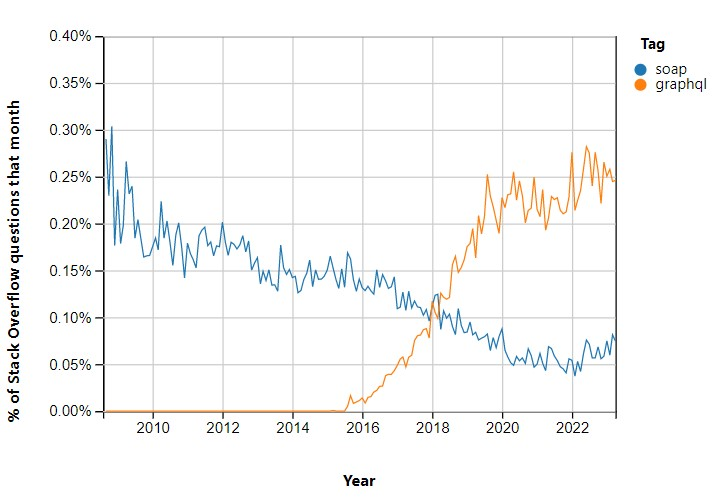
\includegraphics[width=1.0\linewidth]{stackoverflowSOAPGraphQL}
    \caption{Percentage Stack Overflow vragen per maand voor SOAP en GraphQL,\newline
    https://insights.stackoverflow.com/trends?tags=soap\%2Cgraphql}
\end{figure}\\
\nocite{stackoverflowSOAPGraphQL}


\section{REST}

Representational State Transfer, vaker benoemd door middel van het acronym REST, is een type van web API. Deze technologie wordt zeer vaak gebruikt om webservices te bouwen.
Dit zijn applicaties die diensten of data als web resources aanbieden. Door middel van een REST API kan de client om deze resources vragen zonder verder
begrip van de interne werking van de provider. De server reageert dan door een response te versturen met een status code en met de resource in JavaScript object Notation (JSON),
Extensible Markup Language (XML) of andere tekstindelingen. Een web resource is eigenlijk alles waarmee een client op het web kan communiceren.
Het kan betrekking hebben op een bestand, afbeelding, HTML of video. Een resource kan ook een service zijn zoals Google Maps of een financi\"ele dienst.
De API-ontwikkelaars moeten de beslissing maken welke resources ze ondersteunen voor de response.
De API moet de mogelijkheid hebben om de response op te maken op basis van de behoefte van de client.
~\autocite{uptrends}
~\autocite{guru99-webservices}\\

Opdat een API als RESTfull kan worden beschouwd moet het aan enkele kenmerken voldoen.\\
Ten eerste dient het, voor de communicatie, op zijn minst gebruik te maken van het HTTP 1.1 protocol. Het protocol, dat zich in de applicatie laag situeert,
bepaalt dat de client een request, met tekst als vorm, verstuurt naar de server waarop die de gevraagde gegevens terugzendt.
HTTP specificeert verschillende soorten requests methods waaronder GET, POST, PUT en DELETE. Een REST API kan van al deze methods gebruik maken en zal dat
hoogstwaarschijnlijk ook doen. HTTP 1.1 houdt een TCP-connectie open tot er uitdrukkelijk opdracht gegeven wordt om deze te sluiten.
Dit geeft een enorme performantie winst t.o.v. HTTP 1.0. Het nadeel van deze uitdrukkelijke opdracht is dat een wachtende request alle achterliggende requests kan blokkeren.
Extra TCP-connecties kunnen hier een oplossing bieden, deze zijn echter ook gelimiteerd.
~\autocite{w3Protocol}\\
Als tweede kenmerk moet een REST API stateless zijn. Dit houdt in dat er geen informatie zal worden opgeslagen tussen requests door.
De API zal de verbinding tussen server en client verbreken nadat de server een resource in de vorm van een response heeft doorgezonden aan de client.
De API behandelt zo elke request los van een eventuele vorige request. Dit vermindert de hoeveelheid geheugen die een server nodig heeft en verhoogt de
kans op een succesvoller antwoord omdat de server geen extra stappen moet nemen om oude data op te zoeken.\\
Het derde kenmerk voorziet erin dat de verstuurde data cacheable moet zijn. De client weet namelijk a.d.h.v het type van REST request,
meer specifiek de request method, dat hij verzonden heeft wat voor antwoord hij kan verwachten.\\
De vierde eigenschap bestaat uit de verplichting een uniforme interface tussen componenten te voorzien zodat data kan verzonden worden in een standaard vorm.\\
Het vijfde kenmerk specificeert dat het niet noodzakelijk mag zijn dat de client kennis heeft van de verdere werking van de server(s) buiten de vorm van de communicatie zelf.\\
Tot slot laat het zesde, en enige optionele, kenmerk toe om executeerbare code te verzenden indien zo verzocht wordt door de client.
~\autocite{redhat}\\

REST API's zijn flexibel. Ze kunnen requests van verschillende types aan alsook kunnen ze data versturen in verschillende formaten.
Webapplicaties groeien aangezien er telkens meer resources worden toegevoegd. Een REST API zal deze toenemende hoeveelheid van vari\"erende requests snel kunnen behandelen.\\

Een REST API spitst zich steeds toe op het domein dat het als resource zal aanbieden.
Dankzij deze focus en de uniforme manier van werken is het voor een client duidelijk welke functionaliteiten er kunnen worden aangeroepen en hoe dat te doen.
~\autocite{jscrambler}
~\autocite{hubspot}
~\autocite{HTTP1.1vsHTTP2}\\

Afhankelijk van de taal waarin, de tussen server en client, verstuurde data zich bevindt, alsook de programmeertaal van beide applicaties,
zal er bij zowel de client als de server een serialisatieproces moeten plaatsvinden. Er zijn verschillende libraries die de serialisatie kunnnen verzorgen,
zo kan er bij Java gebruik gemaakt worden van bv. Jackson~\parencite{jackson} \newline
Bij de client zal gebruik moeten gemaakt van documentatie van de serverapplicatie of door de endpoints manueel aan te roepen
en zo op basis van de response de mapping voor het serialisatieproces op te maken. Het schrijven van de documentatie,
het cre\"eren van de code in de client om het REST API van de server aan te roepen en zelfs de code in de server kan automatisch gegenereerd worden dankzij
handige hulpmiddelen zoals bv. Swagger~\parencite{swagger}.\\
%TODO JSON vs XML
Tijdens de levensduur van een API is het bijna onvermijdelijk dat er aanpassingen gebeuren. Sommige van deze aanpassingen, zoals het toevoegen van een extra veld aan een object,
hebben geen invloed op eventuele clients en worden daarmee non-breaking changes genoemd. Andere aanpassingen, de zogenaamde breaking changes, hebben als gevolg dat er
fouten kunnen optreeden bij clients. Zo kan het verwijderen van een veld uit een object plots een error veroorzaken bij
een client die het API aanroept en verwacht dat dit veld aanwezig is. In REST API's wordt, wanneer een breaking change geimplementeerd wordt,
meestal gewerkt met een versie verhogen, ook version bump genoemd. De client moet dan bij elke request aangeven welke versie er wordt aangeroepen.
Dit kan door een aparte url per versie, door het versienummer mee te geven in een specifieke request header of door de versie aan de Accept header toe te voegen.
Deze verschillende versies kunnen in dezelfde applicatie gesupporteerd worden of er worden verschillende versies van de applicatie gedeployed.
~\autocite{restversion}\\
%TODO Compressie/GZIP

Wanneer er via een REST API grote datasets beschikbaar worden gesteld wordt het aanzien als best practice om en soort van paginatie te voorzien. Door paginatie te
implementeren kan de grote dataset in kleinere delen worden opgevraagd. Hierdoor zal het systeem minder makkelijk overbelast worden doordat \'e\'en proces lang blijft
hangen wanneer het een request aan het verwerken is. Wanneer de dataset daarboven wordt gebruikt door een applicatie die een user interface voorziet zal het
niet wenselijk zijn om een te grote dataset in \"e\"en keer weer te geven. Dit is immers niet overzichtelijk voor een menselijke gebruiker.
Deze gebruiker zal ook wensen dat de data in enkele seconden wordt weergegeven. Kleinere datasets zullen ook een positief effect hebben op de laadtijd.
Het netwerkverkeer van een applicatie wordt dankzij paginatie ook meer gericht gebruikt voor wat effectief nodig is. Het is ook aangewezen dat een REST API een
default pagina grootte implementeerd voor wanneer deze parameter door de client niet wordt meegegeven. Daarenboven is het beperken van de maximum pagina grootte die
kan opgevraagd worden ook een goed idee.
Praktisch komt paginatie bij een REST API er vaak op neer dat de client een pagina nummer en een pagina grootte meegeeft wanneer er een dataset opgevraagd wordt.
Deze pagina nummer en pagina grootte kan bij een GET request best in de url als query parameters meegegeven worden en bij een POST request eventueel in de request body.
De server zal dan de dataset die wordt verzonden beperken door de items voor de gevraagde pagina over te slaan en alle items na de opgegeven grootte te laten vallen.
Als bijkomende informatie zal de server de dataset aanvullen met pagina informatie. Hier zal het pagina nummer en de pagina grootte steeds toe behoren maar eventueel
ook aangevuld met het totaal aantal items en het totaal aantal pagina's van die grootte.
Stel dat via een REST API een lijst van boeken kan opgevraagd worden via een GET endpoint met page en pageSize query parameters. De request voor de eerste pagina
van 3 boeken zou er dan bijvoorbeeld zo kunnen uitzien:\newline
https://www.hogent.be/boeken?page=0\&pageSize=3
Het antwoord van de server, in JSON formaat, zou dan als volgt kunnen zijn:\newline
\{
''page'': 0,
''pageSize'': 3,
''totalCount'': 50,
''totalPages'': 17,
''results'': [\ldots]
\}\newline
~\autocite{paging}\\
~\autocite{wachtenLaadtijd}\\


\section{gRPC}

Een RPC API stelt een client in staat om op afstand een serverfunctie aan te roepen, zonder dat de client zich verder bewust hoeft te zijn van de interne werking
van de server of de implementatie van de functie.
RPC maakte in het verleden, net zoals REST, gebruik van het HTTP-protocol. De XML-RPC alsook de JSON-RPC implementaties zijn hier voorbeelden van.
Zij maken gebruik van de HTTP request methods GET en POST. De eerste voor het ophalen van data en de tweede voor alle andere functies.\\

De functies van een RPC API kunnen specifiek gericht zijn op de functionaliteit die ze implementeren en daarmee potentieel ook lichtgewicht zijn.
De client moet enkel de naam van de functie specifici\"eren en de vereiste data meegegeven. De response zal ook enkel de data bevatten die door de server nodig wordt geacht.
Wanneer de functies zodanig toegespitst zijn op een functionaliteit wordt er aan de consumer inzicht gegeven over de interne werking van de server,
alsook dient de client vaak kennis te hebben over die interne werking om de functies te kunnen gebruiken.\newline
~\autocite{altexsoft}\\

Google Remote Procedure Calls (gRPC) is de implementatie van Google van het RPC API.\\
Een eerste groot verschil tussen RPC en de implementatie van Google is dat gRPC gebruik maakt van het HTTP 2-transportprotocol.
HTTP 2 werd in 2015 uitgebracht. De doelstellingen bij het ontwikkelen van deze nieuwe versie van het protocol waren vooral toegespitst op performantie.
Hierbij werden enkele nieuwe functies en kenmerken ontwikkeld. Request multiplexing laat toe om requests simultaan te laten gebeuren.
Dankzij Request prioritization kan een prioriteit gegeven worden aan requests. Requests en responses worden nu automatisch gecomprimeerd in tegenselling tot op
uitdrukkelijk verzoek. De mogelijkheid om de verbinding te resetten werd toegevoegd. Daarenboven kan de server ook proactief resources verzenden naar de
cache van clients via de zgn. server push functie. En tot slot is HTTP 2 een binair protocol t.o.v. het op gewone tekst gebaseerde HTTP 1.1 protocol.\newline
~\autocite{baeldung}\\

Het verplicht gebruik van HTTP 2 komt echter ook met het nadeel dat gRPC hierdoor niet ondersteund wordt door de hedendaagse browsers. Javascript heeft geen
volledige controle over HTTP 2 waardoor er bepaalde HTTP 2 functionaliteit, die nodig is voor gRPC, niet beschikbaar is voor browsers die Javascript gebruiken.
Voor gRPC moeten er bijvoorbeeld trailing headers blootgesteld worden welke door browser steeds verborgen worden. Een oplossing hiervoor is het gebruik van een proxy welke
door middel van een normale HTTP request communiceert met de browser en dan de request via gRPC naar de server doorgeeft.\newline
~\autocite{altexsoftgrpc}\\
~\autocite{yukutakahashi}\\

Het HTTP 2 protocol verplicht het gebruik van encryptie, zoals TLS, niet, ondanks hevige discussie in de werkgroep. Het protocol legt wel enige verplichtingen op,
onder meer met betrekking tot het versienummer, wanneer er toch van encryptie of TLS gebruik wordt gemaakt. TLS staat voor Transport Layer Security en is een protocol
dat het encrypteren van data die tussen applicaties over het internet verzonden wordt. Door het dataverkeer te encrypteren zijn de verzender en ontvanger zeker dat
de berichten enkel door hen gelezen kunnen worden alsook dat deze berichten authentiek zijn en van hen afkomstig zijn. TLS wordt voor veel verschillende soorten van internet communicatie gebruikt.
Ondanks het niet verplichten van encryptie in het HTTP 2 protocol wordt TLS in de praktijk toch verplicht wanneer er gebruikt gemaakt wordt van HTTP 2.
Gezien gRPC steeds via het HTTP 2 protocol gaat, zal TLS dan eventueel ook moeten voorzien worden bij gRPC API's. Het gebruik van TLS bij gRPC wordt daarenboven aangeraden.
HTTP 2 wordt door de meeste browsers wel gesupporteerd, maar steeds in combinatie met TLS. Het is niet omdat een browser het HTTP 2 protocol aanvaard dat daarmee gRPC reeds
gesupporteerd wordt.\newline
TLS heeft een impact op de performantie. Bij TLS moet er een onderhandling gevoerd worden met wat heen en weer communicatie. Bij het HTTP 2 protocol ligt dit performantie nadeel,
dankzij het gebruik van multiplexing, lager dan bij HTTP 1.1.
Een server moet een SSL/TLS certificaat hebben om deze encryptie te kunnen gebruiken. Dit certificaat zal in eerste instantie toelaten om de identiteit van het systeem
waarmee een connectie tot stand gebracht wordt te achterhalen en daarna helpen de communicatie over de connectie te encrypteren. Er bestaan zelf gesigneerde certificaten
en CA certificaten gecre\"eerd en gesigneerd door een Certificate Authority. Een self signed certificate wordt normaal alleen geaccepteerd als dit certificaat of de
partij die het getekend heeft gekend is door de consumerende applicatie en dus bijna exclusief voor intern gebruik. CA certificates kunnen geaccepteerd worden indien de
CA zelf vertrouwd wordt door de applicatie.\newline
TLS gaat met deze certificaten symmetrische en assymetrische encryptie toepassen. Via assymmetrische encryptie wordt een beveiligde sessie tussen server en client tot
stand gebracht waarna de uitgewisselde de data via symmetrische encryptie beveiligd wordt. Het proces verloopt als volgt.
\begin{itemize}
    \item De client contacteert de server via HTTPS.
    \item De server verstuurt zijn certificaat en publieke sleutel.
    \item De client verifi\"eert het certificaat met een vertrouwde CA of controleerd of het certificaat zelf vertrouwd wordt.
    \item Client en server onderhandelen over de te gebruiken encryptie.
    \item De client encrypteerd een sessie sleutel, specifiek voor de sessie, door middel van de publieke sleutel en verstuurd deze naar de server.
    \item De server gebruik zijn private sleutel om de sessie sleutel de decrypteren en de sessie wordt vastgesteld.
    \item Client en server gebruiken nu de sessie sleutel om de communicatie de encrypteren en decrypteren.
\end{itemize}
~\autocite{githubhttp2}\\
~\autocite{sslcomhttp2tls}\\
~\autocite{browserhttp2support}\\
~\autocite{tlsBasics}\\
~\autocite{grpctls}\\
~\autocite{http11vshttp2}\\
~\autocite{tlsperformance}\\
~\autocite{sslcertificate}\\
~\autocite{sslhandshake}

gRPC gebruikt geen JSON, XML, of zelfs enig ander teksformaat, maar protocol buffers, ook protobuf genoemd. Protobuf is zodanig geformatteerd dat het niet leesbaar is
voor het menselijk oog. Berichten worden verkleint tot een binair formaat waardoor de snelheid van data transacties hoger zou liggen. gRPC heeft een ingebouwde
protoc-compiler voor het genereren van API-aanroepen en kan zo makkelijk inspelen op vele programmeertalen.
Ondanks deze compiler is een implementatie vaak nog tijdrovender dan alternatieve API's.\newline
~\autocite{googleprotobufguide}\\
~\autocite{dreamfactory}\\

De protoc-compiler genereert de nodige code op basis van een .proto bestand. In dat bestand moet de data structuur alsook de methodes
of functies, die laatsten binnen een Service geplaatst, die het API ter beschikking wilt stellen gedefineerd worden.
De basis data structuur van gRPC zijn messages. Elke message bevat velden
die een vooraf gegaan worden door een .proto primitief type, zie tabel ~\ref{tab:Types}, gevolgd door de naam van het veld en ten slotte een nummer
geassigneerd moeten krijgen. Deze messages dienen zowel voor de request als responses.
gRPC heeft 4 verschillende soorten methodes die kunnen ge\"{\i}mplementeerd worden:
\begin{itemize}
    \item Unary RPCs waarbij de client een enkelvoudige request verstuurd naar de server en ook een enkelvoudige response terugkrijgt.
    \item Server stream RPCs waarbij de client een enkelvoudige request stuurd naar de server maar de server stuurt een stream terug
    waarmee een reeks messages ontvangen kunnen worden.
    \item Client stream RPCs waarbij de client een stream stuurt en de server een enkelvoudige response terug zend.
    \item Bidirectionele stream RPCs waarbij zowel de client als de server een stream verzenden.
\end{itemize}
Op basis van het .proto bestand wordt dan zowel code voor de client als de server gegenereerd. In de server applicatie moeten de methodes die gedeclareerd werden
in het bestand ge\"{\i}mplementeerd worden. De gRPC infrastructuur zal de binnenkomende requests deserialiseren, correcte methodes aanroepen en tot slot ook
de server response serialiseren. In de client wordt er een lokaal object gecre\"eerd, vaak stub of client genoemd, dat dezelfde methodes heeft als de Service in
het .proto bestand. De client applicatie kan dan de methodes van de stub aanroepen en deze zal communicatie met de server applicatie regelen.\newline
~\autocite{grpcintroduction}\\
~\autocite{grpccoreconcepts}\\

\begin{table}
    \centering
    \begin{tabular}{lll}
        \toprule
        \textbf{.proto type} & \textbf{Java Type} & \textbf{C\# Type} \\
        \midrule
        double               & double             & double            \\
        float                & float              & float             \\
        int32                & int                & int               \\
        int64                & long               & long              \\
        uint32               & int                & uint              \\
        uint64               & long               & ulong             \\
        sint32               & int                & int               \\
        sint64               & long               & long              \\
        fixed32              & int                & uint              \\
        fixed64              & long               & ulong             \\
        sfixed32             & int                & int               \\
        sfixed64             & long               & long              \\
        bool                 & boolean            & bool              \\
        string               & String             & string            \\
        bytes                & ByteString         & ByteString        \\
        \bottomrule
    \end{tabular}
    \caption{[Primitieve .proto types]Primitieve .proto types,\newline
    https://protobuf.dev/programming-guides/proto3/\#scalar}
    \label{tab:Types}
\end{table}

gRPC kan synchroon of asynchroon verlopen. Bij synchrone calls zullen de server of client wachten tot de call afgelopen is of ze van de andere applicatie een antwoord gekregen hebben.
Asynchrone calls blokkeren in de applicatie die de call verzonden heeft geen threads. Wanneer er een antwoord komt wordt daarvoor een nieuwe thread opgestart.
De client en server stream RPCs zijn beiden asynchroon. Bij server streaming handelt de client item per item af wanneer deze ontvangen worden en is klaar wanneer alle items ontvangen zijn.
De server is klaar wanneer alle messages verzonden zijn en de status code met eventuele metadata verzonden wordt.
Client streaming verloopt gelijkaardig maar de client verzend de stream naar de server.
Bij bidirectioneel streamen zijn beide streams onafhankelijk van elkaar. Beide applicaties kunnen messages ontvangen en verzenden in elke volgorde.
Ze kunnen wachten op een antwoord maar ook gewoon alle messages continue blijven streamen.
gRPC waarborgt steeds dat de orde waarin de messages via een stream verzonden worden bewaard blijft binnen \'e\'en aangeroepen methode.
Gezien het mogelijk is om eindeloze streams te verzenden is het belangrijk dat beide applicaties de call kunnen be\"eindigen op eigen houtje.\newline
~\autocite{grpccoreconcepts}\\

Een vraag die hierbij naar boven rijst is hoe deze .proto bestanden gedeeld worden tussen client en server applicaties.
Het lijkt erop dat er nog geen algemene best practice over vastgelegd werd. Enkele mogelijke oplossingen
die naar voor gekomen zijn:
\begin{itemize}
    \item In deze blog ~\parencite{protofilesharingSol1} wordt voorgesteld om de gegenereerde code in libraries te verpakken en ter beschikking te stellen van de clients en server applicaties
    \item In het artikel ~\parencite{protofilesharingSol2} wordt een gRPC contract via een REST endpoint gedeeld.
    \item In deze git repository ~\parencite{protofilesharingSol3} wordt voorgesteld om door middel van server reflection clients at runtime requests te laten cre\"eren.
\end{itemize}

gRPC wordt steeds populairder dankzij de opkomst van microservices. Dit zijn services die onafhankelijk van elkaar worden gebouwd en ge\"{\i}mplementeerd om
zo tot een gehele toepassing te komen. Bij een fout in \'e\'en van de services zal dit normaliter enkel de delen van de applicatie verstoren die in aanraking komen
met het deel dat een fout geeft, niet ge\"{\i}mpacteerde services blijven normaal functioneren en dus is niet de hele app verstoord. Bij een monoliet, dit is \"e\"en grote applicate,
kan een kleine fout de hele applicatie breken. Om microservices foutloos met elkaar te laten communiceren zijn er goed gedefinieerde API-contracten nodig.\newline
~\autocite{microsoft}\\

Dankzij de eerder vermelde multiplexing kunnen meerdere dingen tegelijk gebeuren, meerdere requests tegelijk worden verzonden, bij \'e\'en enkele connectie.
Wat hier zeker naar voor treedt is het bidirectioneel streamen. Zowel de client als de server sturen berichten naar elkaar op hetzelfde moment zonder te moeten wachten
op een antwoord. Een client kan zelfs een request annuleren als er geen response meer nodig is van de server.\newline
~\autocite{freecodecamp}\\

Bij gRPC moet er ook rekening gehouden worden met versionering, breaking changes kunnen tot fouten bij clients kunnen leiden.
Bij protobuf zijn er binaire breaking changes die het protoc niet breken maar waarbij de clients wel moeten aangepast worden en protocol breaking changes
die ook effectief het protocol breken en tot gevolg geven dat de clients de status ``UNIMPLEMENTED`` verkrijgt. De versienummer wordt toegevoegd aan
het .proto bestand. Meerdere versies supporteren houdt in dat de applicatie zal moeten gedupliceerd worden.\\

Net zoals bij een REST API is het voor een gRPC API aan best practice dat paging wordt geimplementeerd wanneer er collecties kunnen worden opgehaald.
Google zelf heeft een in haar API design guide een sectie gewijd aan List Pagination~\parencite{googlepaging}. Zelfs indien de verzonden datasets meestal
klein zijn raden ze aan om paginatie te supporteren. De aangegeven rationale is dat wanneer een API paginatie niet supporteert het later
problemen zou kunnen geven om dit toe te voegen gezien het gedrag van het API daarmee gebroken zou worden. Clients zouden zich zo niet bewust zijnn van het feit
dat er dan geen volledig resultaat meer wordt verzonden maar slechts een subset. In de design guide adviseren ze een string veld ''page\_token'' in de request message
van de gRPC functie te voorzien waarmee een specifieke pagina kan opgevraagd worden. Een int32 veld ''page\_size'' om de pagina grootte aan te geven.
En tot slot een string veld ''next\_page\_token'' dat aangeeft of er nog een volgende pagina is en kan gebruikt worden als in het veld ''page\_token''
om die volgende pagina effectief op te vragen.\newline
~\autocite{grpcversion}\\


\section{REST vs gRPC}

Bij het overlopen van de kenmerken van REST en gRPC komen direct enkele belangrijke verschillen naar boven.
Het feit dat REST werkt met het HTTP 1.1 en gRPC met het HTTP 2 protocol heeft ingrijpende gevolgen. HTTP 2 heeft alle mogelijkheden van het 1.1 protocol,
maar voegt daar de hierboven opgesomde functionaliteiten aan toe (Request multiplexing, Request prioritization, Automatic compressing,
Server push en haar binaire vorm). Deze bijkomende functionaliteiten zijn voornamelijk toegespitst op een verbetering van de performantie en effici\"entie van dataoverdracht.
Daarentegen zorgt het gebruik van HTTP 2 door gRPC wel voor het nadeel dat er geen rechtstreekse communicatie met browsers mogelijk is.\newline
~\autocite{cloudflare}\\
~\autocite{tutsplus}\\

Een tweede belangrijk verschil is zichtbaar bij de protocol buffers van gRPC versus het gewone tekst formaat dat gebruikt wordt bij REST-API's.
Dit verschil bouwt duidelijk ook verder op het voorgaande punt m.b.t. het HTTP 1.1 en HTTP 2 protocol.
Protobuf is gelijkaardig aan JSON in die zin dat het beiden programmeer-taal onafhankelijke data uitwisselings formaten zijn.
Protobug gaat verder dan JSON en is eerder een mechanisme voor het serialiseren en de-serialiseren van data.
JSON is leesbaar voor mensen terwijl het binaire formaat bij Protobuf dat niet is~\parencite{json}
Bij deze protocol buffers wordt de datastructuur \'e\'enmaal vastgelegd en gaat de gegenereerde code van gRPC de serialisatie en deserialisatie van de data verzorgen.
Dit serialisatieproces zorgt dat data compact gemaakt wordt voordat ze wordt verzonden wat een performantiewinst zou betekenen.\newline
REST API's hebben echter ook de mogelijkheid om JSON geformateerde data performanter te verzenden. Dankzij de ''Accept-Encoding'' header kan een REST client aangeven
dat de data gecomprimeerd mag worden en met behulp van welk algoritme. De twee standaard waarden voor deze header zijn compress en gzip. Indien de server het aangegeven algoritme
ook ondersteund kan de data zo verzonden worden, de server zal dit ook aangeven met de ''Content-Encoding'' header. Een belangrijk gegeven is dat deze gzip compressie door
nagenoeg alle moderne browsers gesupporteerd wordt.
~\autocite{googleprotobufguide}\\
~\autocite{restcompression}\\
~\autocite{gzipBrowerSupport}\\

Daar staat wel tegenover dat de data, zoals vermeld, steeds vooraf gedefinieerd dient te worden.
Het verzenden van dynamische data maakt het voordeel dat bereikt wordt tijdens de serialisatie namelijk ongedaan.\\

REST heeft een grotere simpliciteit dan gRPC. Er is bij REST enkel een http-compatible client nodig om een applicatie te ontwikkelen terwijl
er bij gRPC steeds protobuf nodig is voor het deserialisatieproces. Toch moet er ook rekening gehouden worden met het feit dat bij REST,
afhankelijk van de programmeertaal waarme gewerkt wordt, ook een serialisatieproces nodig is. Zo words bij Java ondermeer gebruik gemaakt van Jackson.\newline
~\autocite{jackson}

Beide technologi\"en laten toe de server en client volledig van elkaar te scheiden waardoor ze goed schaalbaar zijn.

Breaking changes zijn zowel voor gRPC als REST een mogelijks probleem voor de clients waardoor er met versionering moet gewerkt worden.
REST laat toe verschillende versies te supporteren met \'e\'en applicatie die bepaalde logica herbruikt. Bij gRPC daarentegen wordt code gegenereerd op basis van
het schema waardoor er duplicatie zal zijn bij verschillende versies.\newline
~\autocite{grpcversion}

gRPC is minder wijdverspreid dan REST. Dit geeft voordelen voor REST, gaande van gekende best practices, oplossingen voor allerhande problemen
tot simpelweg ontwikkelaars met ervaring vinden. Kijk maar naar het aantal vragen op stackoverflow voor REST, op vandaag 93395 ~\parencite{stackrest},
versus die voor gRPC, op heden 6110 ~\parencite{stackgrpc}. De grafiek in figuur 2.1 toont wel aan dat het aantal vragen over gRPC in stijgende lijn gaat terwijl
dit voor REST licht dalend is.
\begin{figure}[ht]
    \centering
    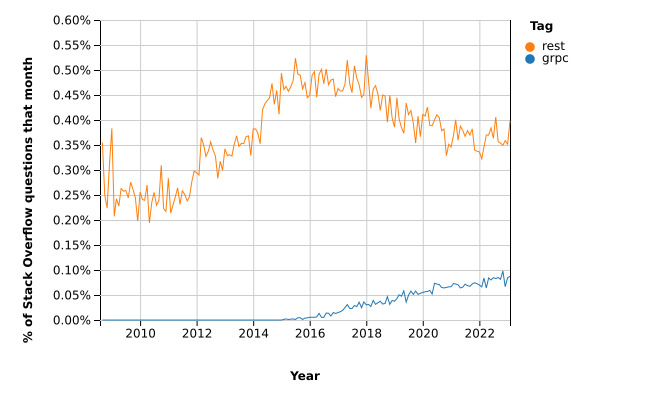
\includegraphics[width=1.0\linewidth]{stackoverflowgrpcrest}
    \caption{Percentage Stack Overflow vragen per maand voor gRPC en REST,\newline
    https://insights.stackoverflow.com/trends?tags=grpc\%2Crest}
\end{figure}\\
\nocite{stackoverflowRESTgRPC}

Tot slot is het ook interessant om deze laatste grafiek nog eens te bekijken, ditmaal echter met alle eerder genoemde API vari\"eteiten.

\begin{figure}[ht]
    \centering
    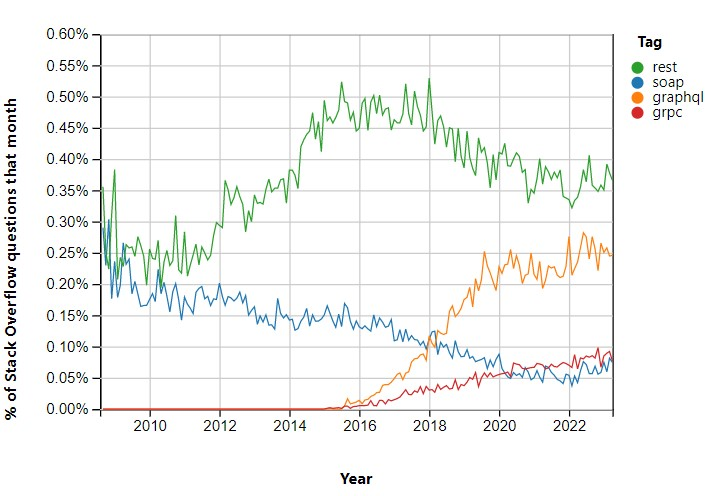
\includegraphics[width=1.0\linewidth]{stackoverflowRESTgRPCSOAPGraphQL}
    \caption{Percentage Stack Overflow vragen per maand voor REST, SOAP GraphQL en gRPC,\newline
    https://insights.stackoverflow.com/trends?tags=grpc\%2Crest}
\end{figure}
\nocite{stackoverflowRESTgRPCSOAPGraphQL}

%XML vs JSON

%%=============================================================================
%% Methodologie
%%=============================================================================

\chapter{\IfLanguageName{dutch}{Methodologie}{Methodology}}%
\label{ch:methodologie}

\section{Inleiding}

Voor het analyseren van het performantieverschil tussen REST en gRPC is er voor beide technologi\"en een server nodig die een API aanbiedt dat geconsumeerd kan worden en
een client die deze server aanroept. Bij dit onderzoek zal de focus niet gelegd worden op het bekomen van benchmark testen waarbij alle factoren die invloed kunnen hebben
zoveel mogelijk vermeden of uitgeschakeld worden. Er wordt getracht een realistisch scenario na te bootsen waarbij, in de parktijk, essenti\"ele stappen van zowel REST als gRPC
ook effectief uitgevoerd worden.
De grootte van de verzonden dataset tegenover de tijdsduur tussen de start en einde van de request, m.a.w. tussen het aanroepen van het API door de client
tot het moment waarop alle gevraagde data bij de client toegekomen is, vormt het belangrijkste vergelijkingspunt.
Er zullen verschillende datasets verstuurd worden opdat kan worden ge\"evalueerd in hoeverre deze grootte een impact heeft op de performantie.
Aangezien er in de praktijk meestal een limiet wordt gezet op de toegelaten reponse body size wordt ook het effect van paginatie in beschouwing genomen.
Voor REST zal het veelgebruikte JSON als serialisatie formaat dienen. Hiernaast zal, met als doel de performantie te optimaliseren,
tevens naar een gecomprimeerd formaat gekeken worden. gRPC zonder gebruik te maken van het serialisatieproces lijkt in de praktijk weinig zinvol te zijn waardoor het geen onderdeel
zal uitmaken van dit vergelijkend onderzoek. Tot slot zal de performantie van gRPC middels een Stream ook vastgelegd worden.\\

\section{Opzet}
\label{sec:opzet}

Zowel de server als client applicatie worden, in aparte modules, in \'e\'en groot Gradle project geplaatst, volgens de principes van Clean Architecture. Hoewel dit
voor een kleine benchmark applicatie wat overkill lijkt, worden zoveel mogelijk best-practices van binnen de codeer wereld gevolgd. Elke applicatie start immers klein.
Gradle is een build automation tool dat ook dependency management verzorgt, waardoor het als alternatief geldt voor Maven en Ant. %TODO op verdeding kunnen we eens vragen "waarom gradle"
Deze twee modules kunnen apart gebuild en gedeployed worden.\newline
~\autocite{Gradle}\\

\paragraph{Server applicatie}

Voor alle stadia van het onderzoek wordt er gebruik gemaakt van een java server applicatie die zowel een REST en gRPC API aanbiedt.
In dit geval zal het gaan om API's die toelaten een lijst van fictieve personen op te vragen. Het aantal personen dat verzonden wordt moet door de client worden aangegeven.
De eerste keer dat een lijst wordt opgevraagd wordt de data gegenereerd en opgeslagen in het geheugen van de applicatie volgens het aantal gevraagde objecten.
Op deze wijze is er zekerheid dat het genereren van de data slechts op de 1e maal dat het API wordt aangereoepen een vertragend effect zal hebben.
Een persoon instantie bevat 5 variabelen die tijdens het genereren van de data m.b.v.\ RandomStringUtils~\parencite{RandomStringUtils}
en RandomDataGenerator~\parencite{RandomDataGenerator} van Apache Commons opgevuld worden met willekeurige tekst of cijfers naargelang het type van variabele.
Voor elk gevraagd aantal zal de eerste request als opwarming dienen en niet worden gebruikt worden als vergelijking.\\

De java applicatie is ontwikkeld met behulp van het Quarkus framework. Quarkus geldt als Cloud-Native Java omdat het een aantal pijnpunten van (voornamelijk) legacy
Spring en SpringBoot projecten gaat tackelen: Bij de opkomst van Cloud Computing hadden de meeste Java applicaties problemen met resources en start-up tijden.
Spring(Boot) applicaties hebben voornamelijk bij de opstart heel veel geheugen nodig, waardoor dit ook moet gereserveerd blijven wanneer de applicatie aan het draaien is.
Hierdoor maak je geen effici\"ent gebruik van je resources met ook hogere kosten als gevolg. Quarkus (en andere Cloud-Native Java frameworks) kent ook een, in vergelijking met Spring,
zeer korte opstarttijd door bijvoorbeeld (in combinatie met GraalVM) ahead-of-time compilatie te voorzien en dode code te verwijderen.
Praktisch kunnen opstarttijden gereduceerd worden tot een paar milliseconden alsook worden de executables (meestal docker images) een heel pak kleiner worden.
Hierdoor kan Java in de cloud terug de concurentie aangaat met scripting talen zoals Python en TypeScript, welke deze opstartproblematiek niet, of alleszins minder, hebben.
Tot slot biedt Quarkus biedt zowel ondersteuning voor REST als voor gRPC, een primaire vereiste voor deze applicatie.\newline
~\autocite{reasonQuarkus}\\
~\autocite{whatisQuarkus}\\
~\autocite{reasonQuarkus2}\\
~\autocite{quarkusAbout}\\

Voor de REST API maakt Quarkus gebruik van RESTEasy, een Jakarta REST-implementatie. Jakarta REST is een REST API-standaard voor Java.
Het serialisatieproces naar JSON gebeurd d.m.v Jackson en gebeurd automatisch door het Quarkus framework.
Het framework voorziet normaal ook in de mogelijkheid om de data te comprimeren voor ze te verzenden.
Het serialiseringsproces naar JSON door Jackson, de compressie en decompressie voor REST alsook het serialisering- en compressieproces bij gRPC zullen telkens opnieuw moeten gebeuren.
Deze processen moeten immers ook deel uitmaken van het vergelijkend onderzoek.
Het REST API wordt voorzien in de klasse People5Resource, boven de definitie van deze klasse wordt een @Path annotatie voorzien waarbij
het eerste deel van de url, ''/people5'', die voor alle endpoints gelijk is, als value wordt meegegeven.
Er worden 3 endpoints aangeboden in dit REST API die zullen aangeroepen worden tijdens de testen. Een GET endpoint ''/people5/\{amount\}'' waarmee een gespecifieerde hoeveelheid
personen kan opgevraagd worden. Dit komt overeen met de methode people5 welke voorzien ook voorzien wordt van een @Path annotatie
die het specifiek voor dat endpoint nodige deel van de url meekrijgt als value nl. ''/\{amount\}''. Amount is hier een path variable. In de variabelen van
de methode moet amount ook geannoteerd worden met @PathParam met hetzelfde value als in de url om het framework deze te laten doorgeven.
Dankzij deze path variable worden bijvoorbeeld 5 personen opgevraagd via een GET request door middel van een variabele in de URI te voorzien b.v.
''people/5'' of ''people/5/compressed''.
Een @GET annotatie wijst aan welke HTTP method naar deze methode geleid moet worden. @Produces zegt welk media type dit endpoint zal retourneren, hier is dat application/json
voor het endpoint zonder compressie en application/octet-stream voor het endpoint voorzien van compressie.
Quarkus zal deze serialisatie automatisch verzorgen. Tot slot annoteren we de method met @Uncompressed om zeker te zijn dat Quarkus zelf hier zeker geen compressie zal toepassen.
Een tweede GET endpoint ''/people5/\{amount\}/compressed'' met dezelfde werking, maar waarbij de data wordt gecomprimeerd alvorens ze wordt verzonden,
wordt met de people5compressed methode gedefinie\"rd. Tijdens het implementeren van beide applicaties bleek Quarkus, ondanks het volgen van de tutorial van Quarkus~\parencite{quarkusgzipcompressie}
en een oplossing van een GitHub discussie~\parencite{quarkusgzipcompressiegithub} uit te proberen, de compressie niet uit te voeren.
Hierdoor is er gekozen de gzip compressie simpelweg zelf te implementeren middels een gzip methode welke grotendeels gebaseerd is op een gevonden voorbeeld van java2s~\parencite{gzipCompressie}.
Deze methode aanvaard een Lijst van generieke objecten en geeft een byte array terug welke de gecomprimeerde data bevat.
Voor beiden wordt de hoeveelheid objecten die geretourneerd moeten worden, aangegeven met een path variabele welke in het URI wordt geplaatst.
Boven elke methode, die overeenkomen met een endpoint, wordt nogmaals een @Path annotatie voorzien die het specifiek voor dat endpoint nodige deel van de url meekrijgt als value.
Via het derde endpoint kan de opgeslagen data, ook cache genaamd, worden leeggemaakt. Dit endpoint kan aangeroepen worden via een POST request naar
de URI van de applicatie aangevuld met ''/people5/cleardata''. Hier worden ook weer een @Path annotatie voorzien met ''/cleardata'', een @POST annotatie om de HTTP method te
specifi\"eren en nog een @Produces met ''application/json'' voor het data formaat aan te geven. Indien de cache wordt leeggemaakt is dit voor beide beschikbare formaten van toepassing.
Dit endpoint geeft een lijst van de eerder opgevraagde hoeveelheden die nu in de cache zitten terug.
Na het leegmaken van de cache zou dit dus steeds een lege lijst moeten zijn.\newline
~\autocite{quarkusREST}\\
~\autocite{Jakarta}\\

Voor het gRPC API wordt gestart vanaf de Quarkus ''tutorial Getting Started With gRPC''~\parencite{quarkusgRPC}.
Bij gRPC moet er een bestand gemaakt worden, met .proto als extensie, waarin alle procedures, welke ter beschikking zijn, worden vastgelegd.
Op basis van dit bestand zal de protocol buffer compiler code genereren.

\begin{figure}[ht]
    \centering
    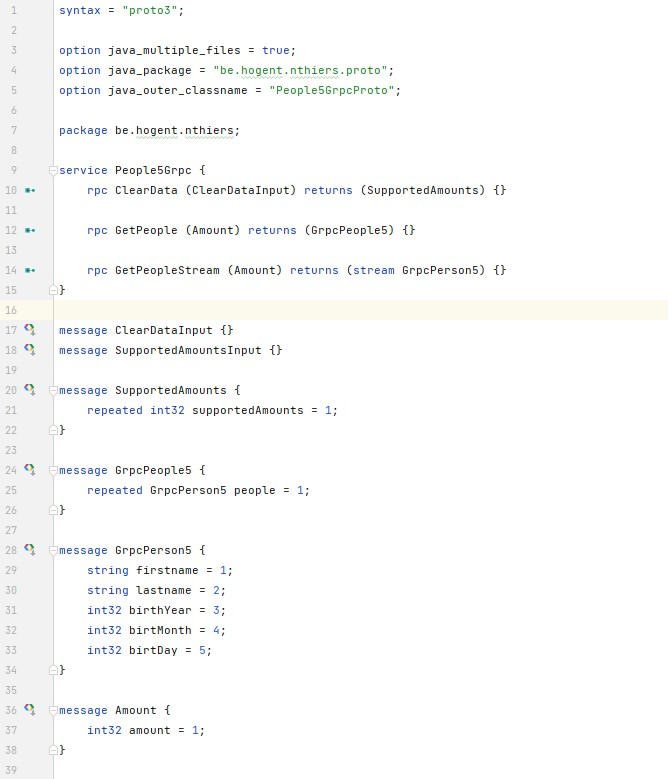
\includegraphics[width=1.0\linewidth]{protobestand}
    \caption{.proto bestand}
\end{figure}

Het bestand start met aan te geven welke syntax gebruikt wordt, in dit geval is dat versie 3, de meest recente versie, van de protocol buffers.
Daarna volgen drie opties die specifek voor java applicaties dienen: ''java\_multiple\_files'', ''java\_package'' en ''java\_outer\_classname''.
java\_multiple\_files staat op true zodat er een apart .java bestand gemaakt wordt voor elke gegenereerde klasse in plaats
van \'e\'en wrapper klass en in nested klasses daarvan alle andere klassen. Bij ''java\_package'' staat niet dezelfde package die in de rest van de applicatie gebruikt is
maar in een proto subpackage zoals aangegeven in de best practices.
Tot slot geeft de ''java\_outer\_classname'' optie aan dat People5GrpcProto moet gebruikt worden als naam voor de wrapper klasse van de service gedefineerd in dit .proto bestand.
Daaronder wordt aangegeven welke package wordt gebruikt voor de gegenereerde code. Dit wordt overschreven door de ''java\_package'' optie die eerder gedefineerd werd maar
in de protobuf Java tutorial~\parencite{protobufJava} wordt vermeld dat er steeds een package moet gedefineerd worden, zelfs bij het gebruik van de optie jav\_package, om naam collisie
te vermijden in de protocol buffer name space. Hierna volgt de effectieve beschrijving van het gRPC API startend met een service interface genaamd People5Grpc waarin
alle beschikbare functies worden gedefineerd. De functie ClearData werkt zoals het eerder beschreven gelijknamige REST endpoint en zorgt dat de cache wordt leeggemaakt.
Met de functie GetPeople kan er een lijst van persoon objecten opgevraagd worden met als waarbij de grootte overeenkomst met de opgegeven hoeveelheid.
Tot slot is er een GetPeopleStream functie die een stream van persoon objecten teruggeeft van het gevraagde aantal.
Na deze functies gedefineerd te hebben moeten de messages die ze ontvangen en verzenden omschreven worden.
ClearDataInput en SupportedAmountsInput zijn lege messages. Er moet steeds een message opgegeven worden voor het return value van een functie.
In plaats van een lege message te defini\"eren kan ook google.protobuf.Empty gebruikt worden, maar dan is het achteraf niet mogelijk om de bestaande functie
te wijzigen in die zin dat ze toch een niet lege message meegeeft. Door een message te beschrijven kunnen hier later nog variabelen aan toegevoegd worden.
Voor dit onderzoek zal dit waarschijnlijk niet nodig zijn maar er wordt toch geopteerd de best practices te respecteren.
SupportedAmounts bevat een lijst van integers, dit wordt aangegeven door het keyword repeated.
Net zoals bij het REST endpoint cleardata zou deze lijst steeds leeg moeten zijn gezien de cache juist werd leeggemaakt.
De message GrpcPeople5 bevat een lijst van GrpcPerson5 messages. GrpcPerson5 geeft het persoon object weer en definieert de 5 variabelen. Als laatste message is er nog
Amount dat als te ontvangen message dient voor de GetPeople en GetPeopleStream functies. Deze message omvat simpelweg een integer die aangeeft hoeveel persoon objecten moeten
verzonden worden.\newline
Op basis van dit .proto bestand zullen de nodige klassen gegenereerd worden. Dit gebeurd tijdens het build proces van Gradle door het commando graldew build -x test.
Deze klassen zijn terug te vinden in de folder ''\textbackslash{}build\textbackslash{}classes\textbackslash{}java\textbackslash{}main'' van de entrypoints-grpc module onder application-server,
in het java package be.hogent.nthiers zoals opgegeven met de java\_package optie. De gegenereerde interface People5Grpc moet nu in de applicatie zelf geïmplementeerd worden.
Hier zal de gRPC API functionaliteit gekoppeld worden aan de achterliggende logica met name de GrpcPeopleCache. De 3 methodes die People5Grpc defineert komen overeen met de 3 functies die
in het .proto bestand zijn opgegeven. Hun return value en method variables zijn ook gegenereerde klassen die de messages van het .proto bestand weerspiegelen.
Deze zijn voorzien van builder waarmee we ze kunnen construeren.\newline
Het gRPC API maakt gebruik van de gegenereerde GrpcPerson5 klasse en dus niet dezelfde klasse als REST. Hierdoor wordt er voor het gRPC API een andere cache gebruikt dan
die van het REST API. Indien dezelfde zou gebruikt worden zouden de Person5 objecten gebruikt voor REST voor de gRPC calls steeds naar GrpcPerson5 objecten gemapt moeten worden
wat de performantie mogelijks negatief zou impacteren. Er zou kunnen geopperd worden dat deze omzetten van het domein object naar de gegenereerde klasse bij een gRPC API steeds nodig
zal zijn en er dus ook rekening mee gehouden dient te worden bij het evalueren van de performantie, het is echter ook bij REST best practice om het domein niet rechtstreeks
via een API bloot te stellen, maar daarentegen om te zetten naar zogenaamde data transfer objects.\newline
~\autocite{quarkusgRPC}\\
~\autocite{DTO}\\
~\autocite{gRPCBestPractices}\\
~\autocite{builderPattern}\\

\begin{figure}[ht]
    \centering
    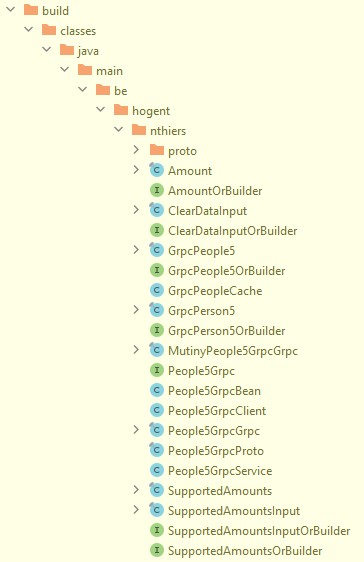
\includegraphics[width=1.0\linewidth]{gegenereerdeklassengrpc}
    \caption{Door protocol buffer compiler gegenereerde klassen}
\end{figure}

Als deployment platform, is er geopteerd om OpenShift te gebruiken. OpenShift geldt als een enterprise ready Kubernetes cluster.
Een Kubernetes cluster is een orchestration tool voor container platforms met onderliggend een set van gelinkte servers (nodes)
waarop containerized applicaties gedeployed kunnen worden.
Entreprise ready duidt op het feit dat OpenShift reeds in een aantal functionaliteiten (security, stabiele upgrades, stabiliteit, \ldots)
voorziet zodat de configuratie opzet en het deployment proces makkelijker verlopen.
Hierdoor zou er sneller moeten gestart kunnen worden met het echte doel nl. het hosten en deployen van de applicatie.
OpenShift heeft ook een administrator en developer view, waarbij vooral de developer view het gemakkelijk maakt om applicaties te gaan deployen
zonder de interne werken van Kubernetes door-en-door te moeten kennen.
Tot slot biedt Red Hat een gratis sandbox aan om een maand lang mee te werken. Verder in de tekst wordt met OpenShift of Kubernetes beiden gerefereerd naar de deploy omgeving
omdat OpenShift uiteindelijk ook gewoon Kubernetes is.\newline
~\autocite{redhatwhatiskubernetes}\\
~\autocite{redhatopenshiftkubernetes}\\
~\autocite{redhatopenshift}

Om een microservice met een REST API in Kubernetes opgezet te krijgen, zijn er drie configuratie bestanden nodig: een deployment config,
een service config en een route config.~\parencite{openshiftDeployment}
\begin{itemize}
    \item Deployment config: bevat onder andere de docker image die gebruikt moet worden, de namespace en de resource reservations zoals geheugen en CPU.
    \item Service config: is de interne DNS binnen Kubernetes en laat applicaties to om andere applicaties via service naam aan te spreken.
    \item Route config: is een config om services extern beschikbaar te stellen. Dit houdt in dat je van buiten de Kubernetes cluster (e.g., web applicatie,
    laptop, \ldots aan je deployment kan)
\end{itemize}

\#Process van opzetten
Kubernetes deployments zijn eenvoudig in een REST context, in een gRPC context bleek het toch iets uitdagender te zijn. Reden: de harde
dependency van gRPC op TLS\/SSL. We moesten de Kubernetes\/OpenShift routes gaan configureren om, in plaat van op de Ingress controllers, TLS
verificatie over te laten aan de deployments (i.e., containers\/PODs). Dit vereiste in een eerste stap dat TLS terminatie van de route
geconfigureerd werd als ''passthrough'' in plaats van ''edge''.

Daarnaast moesten we ook aan gevalideerde certificaten geraken (i.e., gRPC laat geen manueel getekende certificaten toe). Hiervoor maakten we
gebruik van Let's Encrypt om certificaten te genereren. Volgende moeilijkheid: hoe doen we dit binnen een Kubernetes/OpenShift omgeving?
OpenShift\/Kubernetes heeft het concept van operators: dit zijn componenten binnen de cluster die heel wat infrastructuur werk overnemen van jou.
Bepaalde installaties (e.g., Kafka, cert manager, \ldots) worden hierdoor voor jou mogelijk binnen een paar kliks. We installeerden dan de
cert-manager operator, configureerden een issuer en lieten dan een certificate request genereren. Dit request wordt opgeslagen in een Kubernetes
secret en ge\"{\i}njecteerd in een Kubernetes\/OpenShift deployment. Op deze manier krijgt de applicatie direct de nieuwe certificaten toegewezen
wanneer deze opnieuw gegenereerd worden.

Toen dit opgezet was, konden we beginnen aan de deployment, service en route wrap-up\ldots
Het heeft wat zweet gekost, maar uiteindelijk is gRPC aan de praat gekregen op een online Kuberentes\/OpenShift omgeving.
De verschillende resource files kunnen teruggevonden worden in application\_server\/configuration/metadata

De server applicatie wordt gedeployed naaar OpenShift van Red Hat. Op OpenShift is HTTP2 en dus ook gRPC connectiviteit steeds met gebruik van TLS protocol.
Gezien het gebruik van TLS bij gRPC ook als best practice gezien wordt, zoals eerder gemeld in de stand van zaken, zal het hier mee onderdeel uitmaken van performantie testen.\newline
~\autocite{openshifttls}

\paragraph{Client applicatie}

De client applicatie zal klassen voorzien die zowel het REST als gRPC API kunnen aanspreken.
Net zoals bij de server applicatie maakt de client applicatie gebruik van Quarkus.\\

Voor de REST client is er interface die bij Quarkus kenbaar gemaakt wordt als REST client door de @RegisterRestClient annotatie. Deze annotatie wordt ook een configKey meegeven
zodat Quarkus weet welke configuratie moet gebruikt worden voor deze client.  Enkel de url en scope properties zijn hierbij nodig waarbij de url slaat op de url van de
REST API die wordt aangesproken en de scope aangeeft welke CDI scope deze client dient te krijgen, in dit geval Singleton.
Verder wordt de interface zelf voorzien van de @Path annotatie met als String value een deel van de url welke
aan alle endpoints gemeen is, meer specifiek /people5. Elke methode die voorzien wordt in de interface staat voor een endpoint dat kan aangesproken worden.
Boven de clearData methode staat een @POST annotatie waarmee wordt aangegeven dat bij deze methode de POST HTTP-method moet gebruikt worden alsook
nog een @Path annotatie met ´''/cleardata'' als value die de url verder specifieert. De people5 methode krijgt een @GET en een @Path annotatie, waarbij die laatste ''/{amount}''
als value heeft. Deze methode heeft ook een parameter amount welke ook voorzien wordt van een @PathParam annotatie met ''amount'' als value zodat Quarkus
deze parameter als path parameter zal gebruiken. De derde methode people5Compressed is buiten de naam identiek als de people5 methode maar hier gaat het endpoint een
byte array ontvangen wat aangegeven wordt door de @Consumes annotatie voorzien van ''application/octet-stream''. Het omzetten van de byte array naar de java objecten gebeurt
in de test klasse, door middel van de methode gzipDecompressBytes, die gebaseerd is op een simpel voorbeeld van java2s~\parencite{gzipDecompressie}, welke een byte array ontvangt en een lijst van generieke objecten teruggeeft,
en zal nog mee onderdeel zijn van performantiemetingen, ze wordt dus uitgevoerd alvorens het ontvangen van de data geregistreerd wordt in de TestHelper klasse.
~\autocite{quarkusRESTclient}\\

Voor de gRPC client moet weer een .proto bestand voorzien worden op basis waarvan de protocol buffer compiler de nodige code kan genereren. Gemakkelijkheidshalve wordt het
.proto bestand van de server applicatie hier gewoon gekopieerd. In tegenstelling tot in de server applicatie moet er hier geen interface geïmplementeerd worden maar
is er door de generatie een People5Grpc klasse beschikbaar waarmee het gRPC API van de server kan aangesproken worden. Deze klasse kan door gebruik van de
@GrpcClient annotatie geinjecteerd worden in de service klasse welke de functionaliteit verder implementeerd voor gebruik door de testen. Deze annotatie
kan voorzien worden van een String value element name die door Quarkus zal gebruikt worden om de gRPC client te configureren. In de properties worden enkele properties voorzien
die Quarkus nodig heeft. Quarkus weet dankzij de opgegeven element name welke properties hij voor deze specifieke client moet gebruiken.\newline

\begin{itemize}
    \item ''use-quarkus-grpc-client'' wordt op false gezet zodat de gRPC implementatie gebaseerd op Netty gebruikt wordt. Deze werkt op OpenShift.
    \item ''port'' dient om de poort aan te geven via welke de communicatie met het gRPC API zal gebeuren
    \item ''host'' laat toe de url te defineren van de gRPC server
    \item ''ssl.certificate'' geeft de naam van het SSL certificaat welke zich in de recources folder van de client applicatie bevindt
    \item ''max-inbound-message-size'' wordt gebruikt om de standaard maximum message grootte van 4MB te wijzigen
\end{itemize}

Om de gRPC client People5Grpc aan te spreken moeten dezelfde gegenereerde message klassen gebruikt worden als in de server applicatie.
De clearData en de getPeople methode hebben beiden de wrapper klasse ''io.smallrye.mutiny.Uni'' als return type respectievelijk met de gegenereerde klassen
SupportedAmount en GrpcPeople5, deze laatste bevat een lijst met GrpcPerson5 objecten. De getPeopleStream methode daarentegen geeft een ''io.smallrye.mutiny.Multi'' terug.
Zowel Uni als Multi representeren een stream en zijn asynchrone types. Uni omvat slechts \'e\'en item of een fout. Multi omvat 0 tot potentieel oneindig veel items.
Voor Uni zal er gewoon op het item gewacht worden tot dit ontvangen is. Voor een Multi zal er gesubscribed worden en zullen er drie functies nodig zijn om
de items te verwerken. De eerste functie, van het type Consumer~\parencite{Consumer}, gaat elk item verwerken, de tweede functie, weer het type Consumer~\parencite{Consumer},
gaat eventuele failures verwerken en de derde functie, van het type Runnable~\parencite{Runnable} wordt aangeroepen wanneer de call voltooid is.\newline
~\autocite{quarkusgRPCclient}\\
~\autocite{SmallRyeMutiny}\\
~\autocite{MultiSubscribing}\\

De performantie testen worden in dit deel van het project voorzien. De testklasse People5RestServiceTest omvat de performantietesten voor het REST API
en de People5GrpcServiceTest omvat de testen voor het gRPC API. Beiden maken gebruik van een hulpklasse TestHelper de oproepen naar de API's gaat doen,
logs gaat bijhouden en ook het tijdverloop registreren. Voor de constructie van deze hulp klasse moeten drie parameters meegegeven worden nl. een functie
die kan aangeroepen worden om de cache leeg te maken, een object mapper die de objecten naar JSON formaat kan serialiseren en deserialiseren en tot slot de
functie die moet aangeroepen worden om de API calls te doen. Er zijn dan 2 publieke methodes, testPerformance\_singularRequests en testPerformance\_multipleRequests,
die door de testklassen zullen aangeroepen worden. Bij testPerformance\_singularRequests moet de naam van de test meegegeven worden, deze zal bij het wegschrijven
van het logbestand en ook in de logs zelf gebruikt worden, en de lijst van aantallen, in de vorm van een lijst van integers, welke moeten opgevraagd worden
d.m.v. de API call. Eerst wordt de cache eerst leeggemaakt dan wordt de API call tweemaal uitgevoerd zodat de cache voor de specifieke call die getest moet worden
zeker opgevuld is en zodat de server opgewarmd is. Daarna wordt de performantie gestest door de tijd te registreren dan de call nogmaals uit te voeren.
Wanneer het antwoord ontvangen is wordt de tijdsduur vastgelegd. Bij de REST calls wordt de ontvangen lijst van personen nogmaals geserialiseerd naar JSON
en naar een file weggeschreven om zo de grootte van de dataset in JSON formaat te kunnen registreren.
Tot slot gaat de TestHelper ook de logs, met daarin het resultaat van de performantietest, wegschrijven naar een file.
De tweede methode testPerformance\_multipleRequests verwacht ook de testnaam, een lijst van amounts en daarnaast nog een integer genaamd batchSize.
Tijdens het uitvoeren van deze method zullen de opgegeven aantallen opgehaald worden door middel van de API call meermaals uit te voeren met de batchSize als aantal
tot het totale gevraagd aantal is ontvangen. Ook hier wordt de tijd geregistreerd, maar dan van het ophalen van het volledige aantal d.m.v.
verschillende calls van de opgegeven batch grootte.\\

De hele opzet in deze methodiek kan een effect hebben op de resultaten die zullen bekomen worden. Het wijzigen ervan zal dus kunnen maken dat de resultaten afwijken.
Bij het beschouwen van de hierbij geregistreerde performantieverschillen moet daar rekening mee gehouden worden. Grote verschillen en verhouding tussen resultaten zullen echter
ook na aanpassing van de testmodaliteiten gelijkaardig blijven, waardoor het nog mogelijk zal zijn conclusie te maken en voordeel te halen uit dit onderzoek.\\

De broncode van dit project, dat zowel de server als client applicatie omvat, is publiek beschikbaar op Github via https://github.com/thiersnicolas/gRPC\_vs\_REST.git

\section{Enkelvoudige requests}
\label{enkelvoudigerequestsmethodologie}

Uit de eerdere uitleg over de implementatie van de TestHelper klasse zal al enigzins duidelijk geworden zijn hoe de performantie testen gaan verlopen.
Er wordt gestart met de performantie te evalueren van enkelvoudige requests voor welbepaalde sets van data voor alle geïmplementeerde API calls.
Het doel is vast te leggen hoe de verhouding van het tijdsverloop tussen de verschillende API calls is en hoe deze evolueert naargelang de
datasets groter of kleiner zijn.\\

De API calls die zullen worden uitgevoerd:
\begin{itemize}
    \item REST API: GET people5
    \item REST API
    \item gRPC getPeople
    \item gRPC getPeopleStream
\end{itemize}

Tabel~\ref{tab:Gevraagdedatasets} geeft de datasets weer die zullen opgevraagd worden, hiervoor werd reeds gekeken wat hun grootte is
wanneer ze in JSON formaat naar een bestand worden weggeschreven (deze grootte kan zeer kleine verschillen vertonen welke nagenoeg geen impact zullen hebben op de performantie).
Alle datasets zullen vier maal opgevraagd worden waarna het gemiddelde van deze vier tijdsverlopen genomen wordt om de verschillende soorten API calls te gaan vergelijken.\\

\begin{table}
    \centering
    \begin{tabular}{rrll}
        \toprule
        \textbf{Aantal personen} & \textbf{Grootte (bytes)} & \textbf{Grootte (KB)} & \textbf{Grootte (MB)} \\
        \midrule
        1024 & 89028 & 86,94 & 0,08 \\
        2048 & 178062 & 173,89 & 0,17 \\
        4096 & 356103 & 347,76 & 0,34 \\
        8192 & 712225 & 695,53 & 0,68 \\
        9216 & 801209 & 782,43 & 0,76 \\
        10240 & 890124 & 869,26 & 0,85 \\
        11264 & 979136 & 956,19 & 0,93 \\
        12288 & 1068188 & 1043,15 & 1,02 \\
        13312 & 1157125 & 1130 & 1,1 \\
        14336 & 1246294 & 1217,08 & 1,19 \\
        15360 & 1335174 & 1303,88 & 1,27 \\
        16384 & 1424160 & 1390,78 & 1,36 \\
        20480 & 1780317 & 1738,59 & 1,7 \\
        24576 & 2136595 & 2086,52 & 2,04 \\
        28672 & 2492585 & 2434,17 & 2,38 \\
        32768 & 2848302 & 2781,54 & 2,72 \\
        36864 & 3204548 & 3129,44 & 3,06 \\
        40960 & 3560626 & 3477,17 & 3,4 \\
        45056 & 3916542 & 3824,75 & 3,74 \\
        49152 & 4272567 & 4172,43 & 4,07 \\
        53248 & 4628732 & 4520,25 & 4,41 \\
        57344 & 4984625 & 4867,8 & 4,75 \\
        61440 & 5341250 & 5216,06 & 5,09 \\
        65536 & 5697065 & 5563,54 & 5,43 \\
        131072 & 11394036 & 11126,99 & 10,87 \\
        262144 & 22788054 & 22253,96 & 21,73 \\
        524288 & 45575493 & 44507,32 & 43,46 \\
        \bottomrule
    \end{tabular}
    \caption{Gevraagde Datasets}
    \label{tab:Gevraagdedatasets}
\end{table}

Voor de 2 REST calls en de getPeople functie van het gRPC API is het simpelweg bovenstaande lijst door te geven aan de testPerformance\_singularRequests methode
van de TestHelper. De getPeopleStream methode van het gRPC API geeft een object van het type Multi terug, waarover eerder reeds meer informatie werd gegeven.
Om deze methode te testen is er een nieuwe functie gemaakt welke door middel van een AtomicInteger de tel bijhoudt van alle ontvangen items en bij het voltooien van
de gRPC functie een AtomicBoolean op true zet. Wanneer die AtomicBoolean op true staat wordt de controle teruggegeven aan de TestHelper. Hieruit bleek dat effectief
alle gevraagde items ontvangen werden. Om een correcte performantiemeting te kunnen doen dient de AtomicInteger terug verwijderd te worden gezien deze de metingen
negatief be\"{\i}nvloedt\"\\. De AtomicBoolean wordt enkel en slechts eenmaal opgeroepen wanneer de oproep voltooid is waardoor de impact hiervan nagenoeg geen impact zal hebben.

\section{Meervoudige requests}

In deze volgende onderzoeksfase wordt er meer rekening gehouden met eventuele praktische beperkingen waarmee applicatie kunnen en zullen geconfronteerd worden.
Zo zal het beschikbare geheugen van een applicatie alsook het aantal simultane requests die mogelijks zullen ontvangen worden het noodzakelijk maken om
de toegelaten response grootte te beperken. Voor REST wordt er in dergelijke gevallen vaak voor het pagineren van datasets geopteerd.
Hierbij is de verstuurde dataset slechts een deel van het geheel. De client geeft bij een gepagineerde request aan hoe groot de subset moet zijn
en het hoeveelste deel deze subset is van de gehele dataset. De server geeft de gevraagde subset aangevuld door de subset grootte, de positie t.o.v. de gehele set
en tot slot ook de grootte van de gehele lijst.\\

Praktisch wordt hier de testPerformance\_multipleRequests van de TestHelper klasse aangeroepen voor alle REST API calls en de getPeople functie van het gRPC API.
Het tijdsverloop van alle calls, met de opgegeven batch grootte, tot de gehele dataset ontvangen is, zal worden geregistreed. Eerst zullen verschillende batch groottes
uitgetest worden om te evalueren wat de impact van deze grootte is op de performantie. Een grote batch heeft immers tot gevolg dat er minder calls zullen moeten uitgevoerd worden.\newline
Tabel ~\ref{tab:Batches} geeft aan welke batches zullen worden gebruikt. Het totale aantal items die worden opgevraagd bedraagd 4.194.304 welke een grootte hebben
van 347,68 MB wanneer ze zijn weggeschreven in JSON formaat naar een bestand. De hoogste snelheid waarmee deze grote dataset , door middel van batched calls, kon worden
opgehaald zal dan vergeleken worden tussen de verschillende API's en verschillende formaten of methodes\\

getPeopleStream van het gRPC API is hier weer het vreemde eendje waarbij het pagineren van de calls zinloos is. De server zal immers de beschikbare capaciteit gebruiken
om item per item door te sturen, gebruik makend van de HTTP2 functionaliteit, zolang de client niet blokkeert. Voor getPeopleStream zal de testPerformance\_singularRequests methode van
de TestHelper klasse gebruikt worden voor de totale grootte die ook bij de andere API calls wordt opgevraagd.
De performantie hiervan kan dan correct vergeleken worden met de andere resultaten.\\

\begin{table}
    \centering
    \begin{tabular}{rrrll}
        \toprule
        \textbf{Aantal calls} & \textbf{Items / call} & \textbf{Grootte batch (bytes)} & \textbf{Grootte batch (KB)} & \textbf{Grootte batch (MB)} \\
        \midrule
        4096 & 1024 & 89028 & 86,94 & 0,08 \\
        2048 & 2048 & 178062 & 173,89 & 0,17 \\
        1024 & 4096 & 356103 & 347,76 & 0,34 \\
        512 & 8192 & 712225 & 695,53 & 0,68 \\
        456 & 9216 & 801209 & 782,43 & 0,76 \\
        410 & 10240 & 890124 & 869,26 & 0,85 \\
        373 & 11264 & 979136 & 956,19 & 0,93 \\
        342 & 12288 & 1068188 & 1043,15 & 1,02 \\
        316 & 13312 & 1157125 & 1130 & 1,1 \\
        293 & 14336 & 1246294 & 1217,08 & 1,19 \\
        274 & 15360 & 1335174 & 1303,88 & 1,27 \\
        256 & 16384 & 1424160 & 1390,78 & 1,36 \\
        205 & 20480 & 1780317 & 1738,59 & 1,7 \\
        171 & 24576 & 2136595 & 2086,52 & 2,04 \\
        147 & 28672 & 2492585 & 2434,17 & 2,38 \\
        128 & 32768 & 2848302 & 2781,54 & 2,72 \\
        114 & 36864 & 3204548 & 3129,44 & 3,06 \\
        103 & 40960 & 3560626 & 3477,17 & 3,4 \\
        94 & 45056 & 3916542 & 3824,75 & 3,74 \\
        86 & 49152 & 4272567 & 4172,43 & 4,07 \\
        79 & 53248 & 4628732 & 4520,25 & 4,41 \\
        74 & 57344 & 4984625 & 4867,8 & 4,75 \\
        69 & 61440 & 5341250 & 5216,06 & 5,09 \\
        64 & 65536 & 5697065 & 5563,54 & 5,43 \\
        32 & 131072 & 11394036 & 11126,99 & 10,87 \\
        16 & 262144 & 22788054 & 22253,96 & 21,73 \\
        8 & 524288 & 45575493 & 44507,32 & 43,46 \\
        \bottomrule
    \end{tabular}
    \caption{Batches}
    \label{tab:Batches}
\end{table}

\section{Reproduceren}
Alle testen die in deze methodiek beschreven zijn kunnen gereproduceerd worden met behulp van de beschreven server en client applicaties.\\
Zoals eerder aangegeven is de broncode terug te vinden is op de publieke GIT repository op Github via https://github.com/thiersnicolas/gRPC\_vs\_REST.git.
De server applicatie is op heden gedeployed op OpenShift en zal maar tijdelijk beschikbaar blijven voor de duur van dit onderzoek.
Deze applicatie kan echter gemakkelijk opnieuw gedeployed worden op OpenShift dankzij de uitleg in sectie ~\ref{sec:opzet} onder paragraaf Server applicatie.
Voor andere cloud omgeving kan het zijn dat er bijkomende aanpassingen nodig zijn aan de broncode.\\
De client applicatie kan gewoon lokaal gebruikt worden door de gemaakte testen op te starten. Deze zullen .txt bestanden genereren welke de metingen bevatten.





%%=============================================================================
%% Bevindingen
%%=============================================================================

\chapter{\IfLanguageName{dutch}{Bevindingen}{Findings}}%
\label{ch:bevindingen}

\section{Enkelvoudige requests}

De resultaten van de performantie testen voor de enkelvoudige requests met het REST API zonder compressie zijn terug te vinden in tabel ~\ref{tab:RESTenkelvoudigtabel}.
Elke lijn op deze tabel komt overeen met een uitgevoerde request. In de eerste kolom worden het aantal items die werden opgevraagd weergegeven,
in de tweede tot de vierde kolom de grootte van de dataset, in respectievelijk bytes, KB en MB, wanneer ze in JSON formaat naar een file worden weggeschreven,
daarna het tijdsverloop tussen de start van de request en het verkrijgen van de opgevraagde data in millie seconden. De zesde kolom geeft de de grootte van de
verzonden dataset per seconde dat de request geduurd heeft. Deze set van requests werd tweemaal uitgevoerd, in de laatste twee kolommen staat het resultaat, nl. het tijdsverloop en de snelheid,
van deze tweede set requests.
Op figuur ~\ref{fig:RESTenkelvoudigeRequestsFig} wordt de snelheid in MB/sec weergegeven ten opzichte van de grootte van de dataset. Hier werd tevens een trendlijn voorzien.

\begin{table}
    \centering
    \begin{tabular}{llllllll}
        \toprule
        \textbf{} & \textbf{} & \textbf{} & \textbf{} & \textbf{22/05/2023} & \textbf{} & \textbf{22/05/2023} & \textbf{} \\
        \midrule
        Items / call & Grootte set (bytes) & Grootte set (KB) & Grootte set (MB) & tijdsverloop (millies) & snelheid (Mb/s) & tijdsverloop (millies) & snelheid (Mb/s) \\
        1024 & 89028 & 86,94 & 0,08 & 67 & 1,194029851 & 69 & 1,15942029 \\
        2048 & 178062 & 173,89 & 0,17 & 131 & 1,297709924 & 130 & 1,307692308 \\
        4096 & 356103 & 347,76 & 0,34 & 223 & 1,524663677 & 261 & 1,302681992 \\
        8192 & 712225 & 695,53 & 0,68 & 429 & 1,585081585 & 445 & 1,528089888 \\
        9216 & 801209 & 782,43 & 0,76 & 470 & 1,617021277 & 473 & 1,606765328 \\
        10240 & 890124 & 869,26 & 0,85 & 525 & 1,619047619 & 533 & 1,594746717 \\
        11264 & 979136 & 956,19 & 0,93 & 608 & 1,529605263 & 587 & 1,584327087 \\
        12288 & 1068188 & 1043,15 & 1,02 & 627 & 1,626794258 & 629 & 1,621621622 \\
        13312 & 1157125 & 1130 & 1,1 & 689 & 1,596516691 & 681 & 1,615271659 \\
        14336 & 1246294 & 1217,08 & 1,19 & 789 & 1,508238276 & 752 & 1,582446809 \\
        15360 & 1335174 & 1303,88 & 1,27 & 784 & 1,619897959 & 784 & 1,619897959 \\
        16384 & 1424160 & 1390,78 & 1,36 & 832 & 1,634615385 & 836 & 1,626794258 \\
        20480 & 1780317 & 1738,59 & 1,7 & 1037 & 1,639344262 & 1057 & 1,608325449 \\
        24576 & 2136595 & 2086,52 & 2,04 & 1284 & 1,588785047 & 1297 & 1,572860447 \\
        28672 & 2492585 & 2434,17 & 2,38 & 1444 & 1,648199446 & 1723 & 1,381311666 \\
        32768 & 2848302 & 2781,54 & 2,72 & 1689 & 1,610420367 & 1673 & 1,625821877 \\
        36864 & 3204548 & 3129,44 & 3,06 & 1874 & 1,632870864 & 2465 & 1,24137931 \\
        40960 & 3560626 & 3477,17 & 3,4 & 2082 & 1,633045149 & 5177 & 0,656751014 \\
        45056 & 3916542 & 3824,75 & 3,74 & 2278 & 1,641791045 & 2278 & 1,641791045 \\
        49152 & 4272567 & 4172,43 & 4,07 & 2511 & 1,62086818 & 2612 & 1,558192956 \\
        53248 & 4628732 & 4520,25 & 4,41 & 2693 & 1,637578908 & 2737 & 1,611253197 \\
        57344 & 4984625 & 4867,8 & 4,75 & 3248 & 1,462438424 & 2888 & 1,644736842 \\
        61440 & 5341250 & 5216,06 & 5,09 & 3093 & 1,645651471 & 3128 & 1,627237852 \\
        65536 & 5697065 & 5563,54 & 5,43 & 3944 & 1,376774848 & 3351 & 1,620411817 \\
        131072 & 11394036 & 11126,99 & 10,87 & 8771 & 1,239311367 & 6707 & 1,620694796 \\
        262144 & 22788054 & 22253,96 & 21,73 & 13460 & 1,614413076 & 13412 & 1,620190874 \\
        524288 & 45575493 & 44507,32 & 43,46 & 28082 & 1,547610569 & 32374 & 1,342435288 \\
         &  &  &  &  &  &  &  \\
         &  &  & gemiddelde: &  & 1,551567585 &  & 1,50085742 \\
         &  &  & max: &  & 1,648199446 &  & 1,644736842 \\
         &  &  & min: &  & 1,194029851 &  & 0,656751014 \\
        \bottomrule
    \end{tabular}
    \caption{REST enkelvoudige requests}
    \label{tab:RESTenkelvoudigtabel}
\end{table}


\begin{figure}[ht]
    \centering
    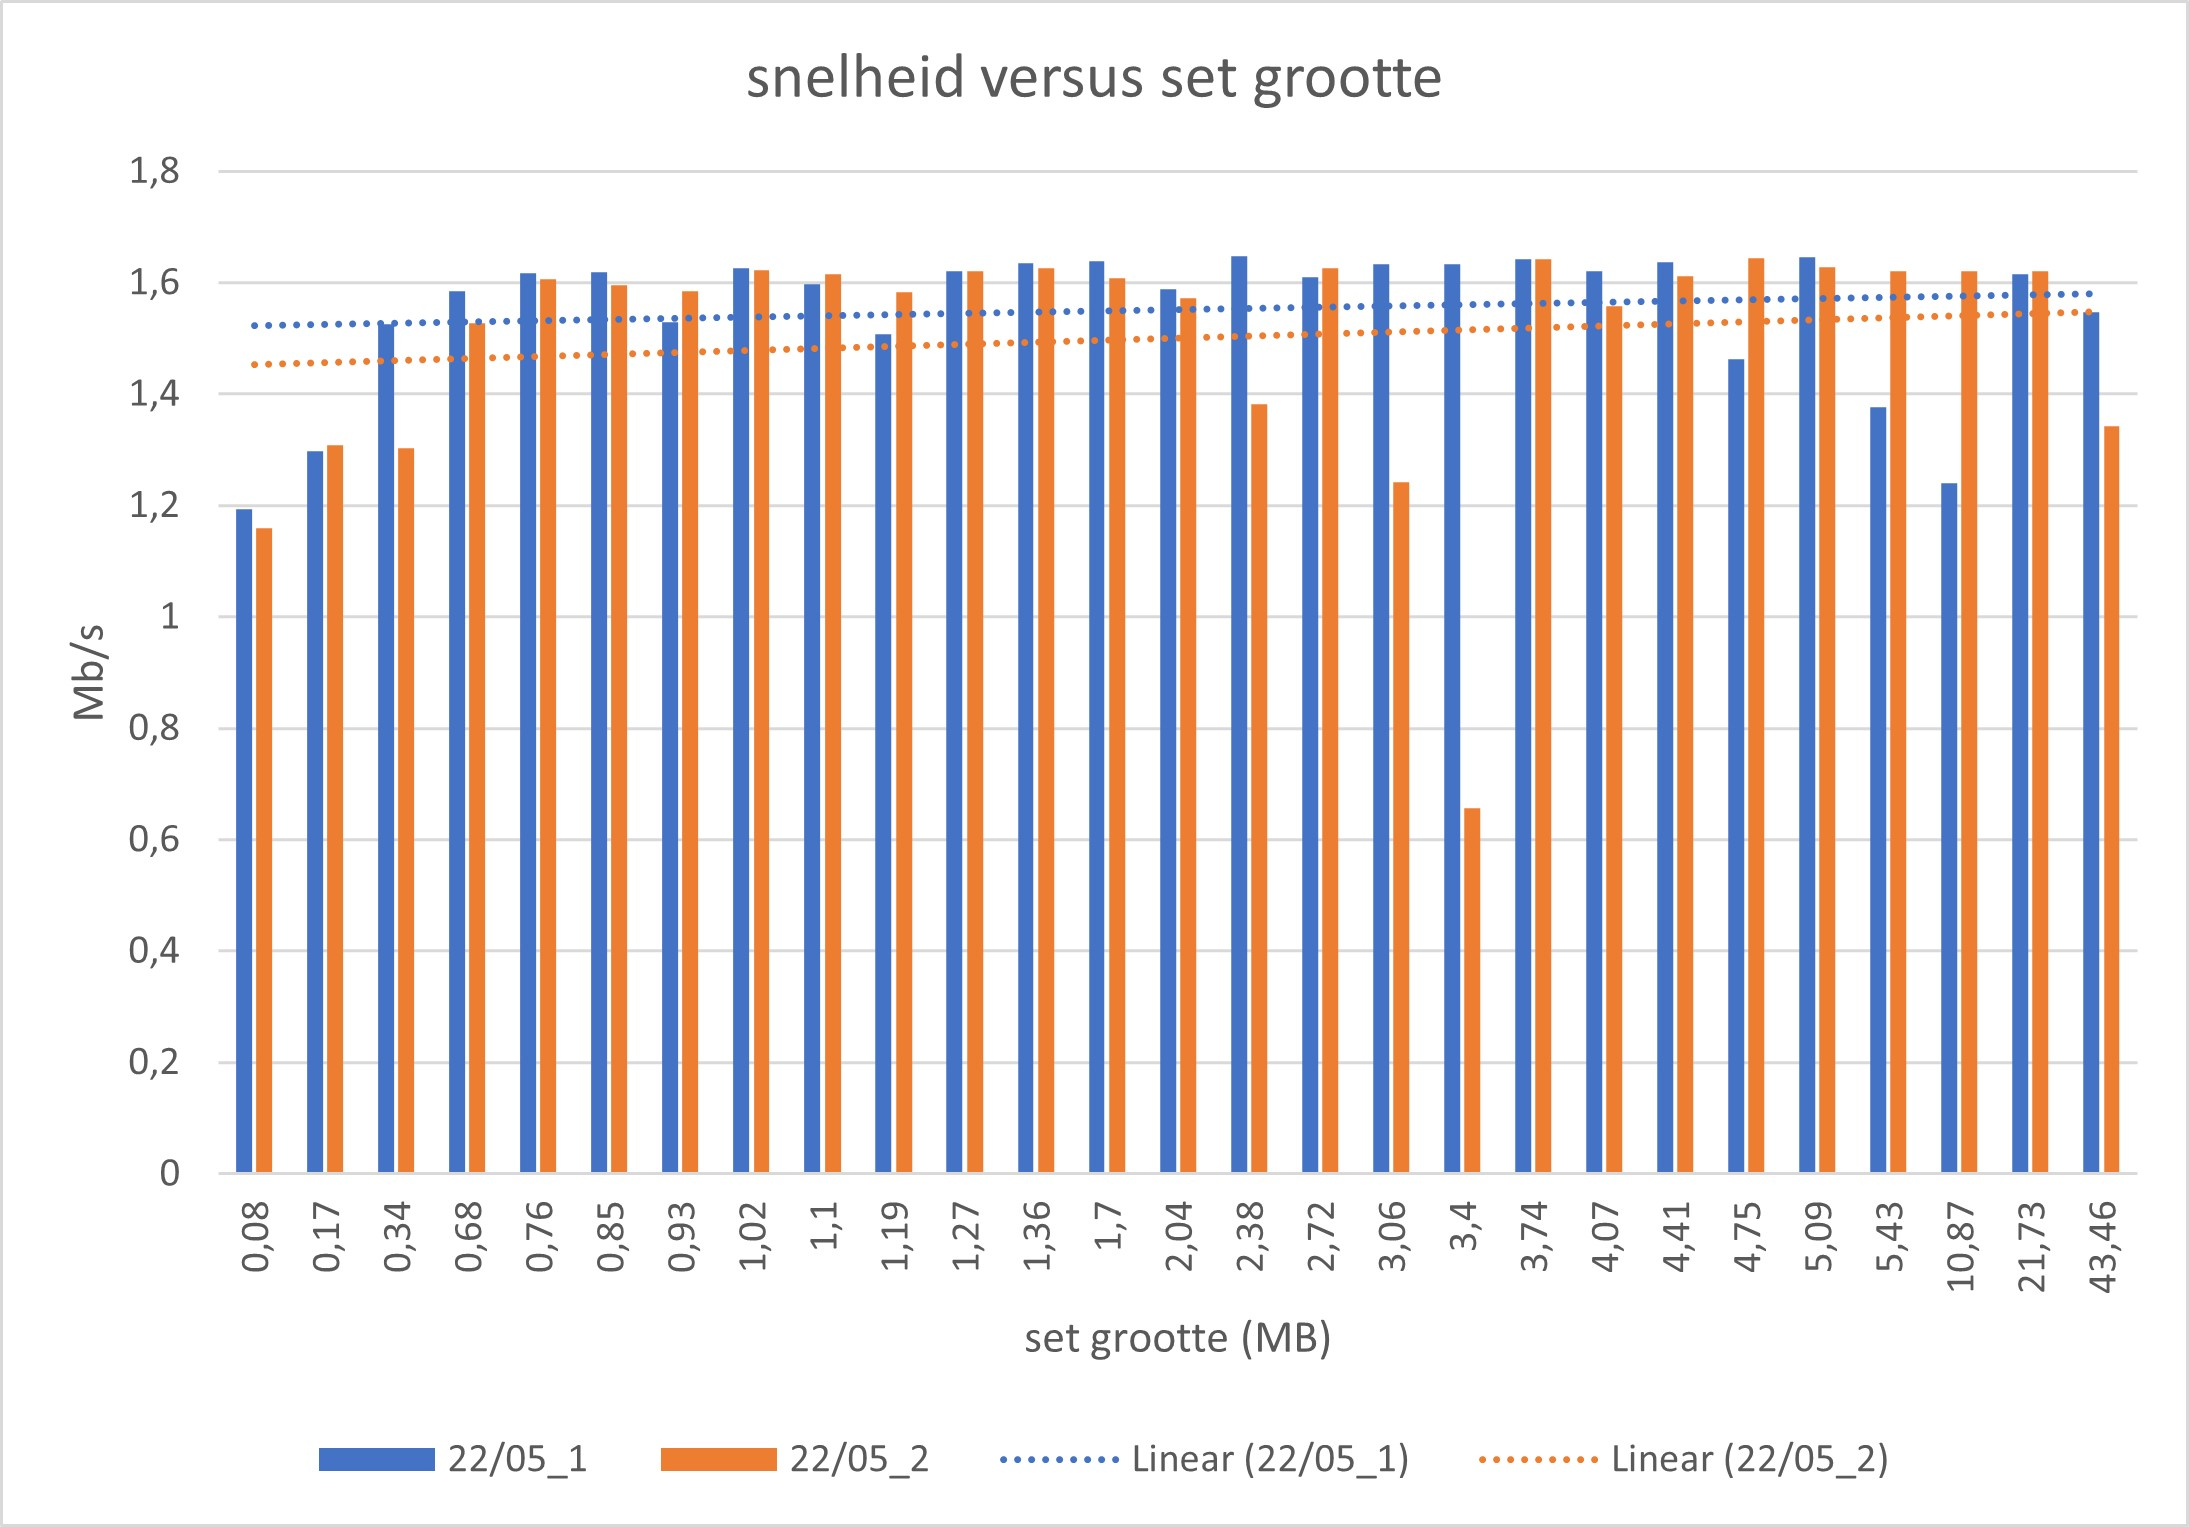
\includegraphics[width=1.0\linewidth]{RESTenkelvoudigeRequests}
    \caption{[REST enkelvoudige requests snelheid vs. grootte dataset]REST enkelvoudige requests snelheid vs. datasets van vari\"erende grootte}
    \label{fig:RESTenkelvoudigeRequestsFig}
\end{figure}

De resultaten van de performantie testen voor de enkelvoudige requests met de gRPC API functie getPeople, welke een object van het type Uni teruggeeft zijn
terug te vinden in tabel ~\ref{tab:gRPCUnienkelvoudigtabel}.
Op figuur ~\ref{fig:gRPCUnienkelvoudigeRequestsFig} wordt de snelheid \(MB/sec\) weergegeven ten opzichte van de grootte van de dataset. Hier werd tevens een trendlijn voorzien.


\begin{table}
    \centering
    \begin{tabular}{llllllll}
        \toprule
        \textbf{} & \textbf{} & \textbf{} & \textbf{} & \textbf{22/05/2023} & \textbf{} & \textbf{22/05/2023} & \textbf{} \\
        \midrule
        Items / call & Groote subset (bytes) & Groote subset (KB) & Groote subset (MB) & tijdsverloop (millies) & snelheid (Mb/s) & tijdsverloop (millies) & snelheid (Mb/s) \\
        1024 & 89028 & 86,94 & 0,08 & 48 & 1,666666667 & 66 & 1,212121212 \\
        2048 & 178062 & 173,89 & 0,17 & 64 & 2,65625 & 78 & 2,179487179 \\
        4096 & 356103 & 347,76 & 0,34 & 84 & 4,047619048 & 76 & 4,473684211 \\
        8192 & 712225 & 695,53 & 0,68 & 138 & 4,927536232 & 138 & 4,927536232 \\
        9216 & 801209 & 782,43 & 0,76 & 233 & 3,261802575 & 152 & 5 \\
        10240 & 890124 & 869,26 & 0,85 & 194 & 4,381443299 & 177 & 4,802259887 \\
        11264 & 979136 & 956,19 & 0,93 & 194 & 4,793814433 & 190 & 4,894736842 \\
        12288 & 1068188 & 1043,15 & 1,02 & 229 & 4,454148472 & 204 & 5 \\
        13312 & 1157125 & 1130 & 1,1 & 217 & 5,069124424 & 220 & 5 \\
        14336 & 1246294 & 1217,08 & 1,19 & 239 & 4,979079498 & 232 & 5,129310345 \\
        15360 & 1335174 & 1303,88 & 1,27 & 251 & 5,059760956 & 258 & 4,92248062 \\
        16384 & 1424160 & 1390,78 & 1,36 & 266 & 5,112781955 & 263 & 5,171102662 \\
        20480 & 1780317 & 1738,59 & 1,7 & 331 & 5,135951662 & 325 & 5,230769231 \\
        24576 & 2136595 & 2086,52 & 2,04 & 394 & 5,177664975 & 401 & 5,087281796 \\
        28672 & 2492585 & 2434,17 & 2,38 & 453 & 5,253863135 & 455 & 5,230769231 \\
        32768 & 2848302 & 2781,54 & 2,72 & 516 & 5,271317829 & 575 & 4,730434783 \\
        36864 & 3204548 & 3129,44 & 3,06 & 581 & 5,266781411 & 576 & 5,3125 \\
        40960 & 3560626 & 3477,17 & 3,4 & 649 & 5,238828968 & 639 & 5,320813772 \\
        45056 & 3916542 & 3824,75 & 3,74 & 707 & 5,289957567 & 695 & 5,381294964 \\
        49152 & 4272567 & 4172,43 & 4,07 & 766 & 5,313315927 & 794 & 5,125944584 \\
        53248 & 4628732 & 4520,25 & 4,41 & 826 & 5,338983051 & 819 & 5,384615385 \\
        57344 & 4984625 & 4867,8 & 4,75 & 895 & 5,30726257 & 909 & 5,225522552 \\
        61440 & 5341250 & 5216,06 & 5,09 & 1036 & 4,913127413 & 1612 & 3,157568238 \\
        65536 & 5697065 & 5563,54 & 5,43 & 1047 & 5,186246418 & 1266 & 4,289099526 \\
        131072 & 11394036 & 11126,99 & 10,87 & 2009 & 5,410652066 & 2030 & 5,354679803 \\
        262144 & 22788054 & 22253,96 & 21,73 & 4162 & 5,221047573 & 4080 & 5,325980392 \\
        524288 & 45575493 & 44507,32 & 43,46 & 8931 & 4,866196395 & 9030 & 4,812846069 \\
         &  &  &  &  &  &  &  \\
         &  &  &  & gemiddelde: & 4,763008315 &  & 4,728994056 \\
         &  &  &  & max: & 5,410652066 &  & 5,384615385 \\
         &  &  &  & min: & 1,666666667 &  & 1,212121212 \\
        \bottomrule
    \end{tabular}
    \caption{gRPC Uni enkelvoudige requests}
    \label{tab:gRPCUnienkelvoudigtabel}
\end{table}

\begin{figure}[ht]
    \centering
    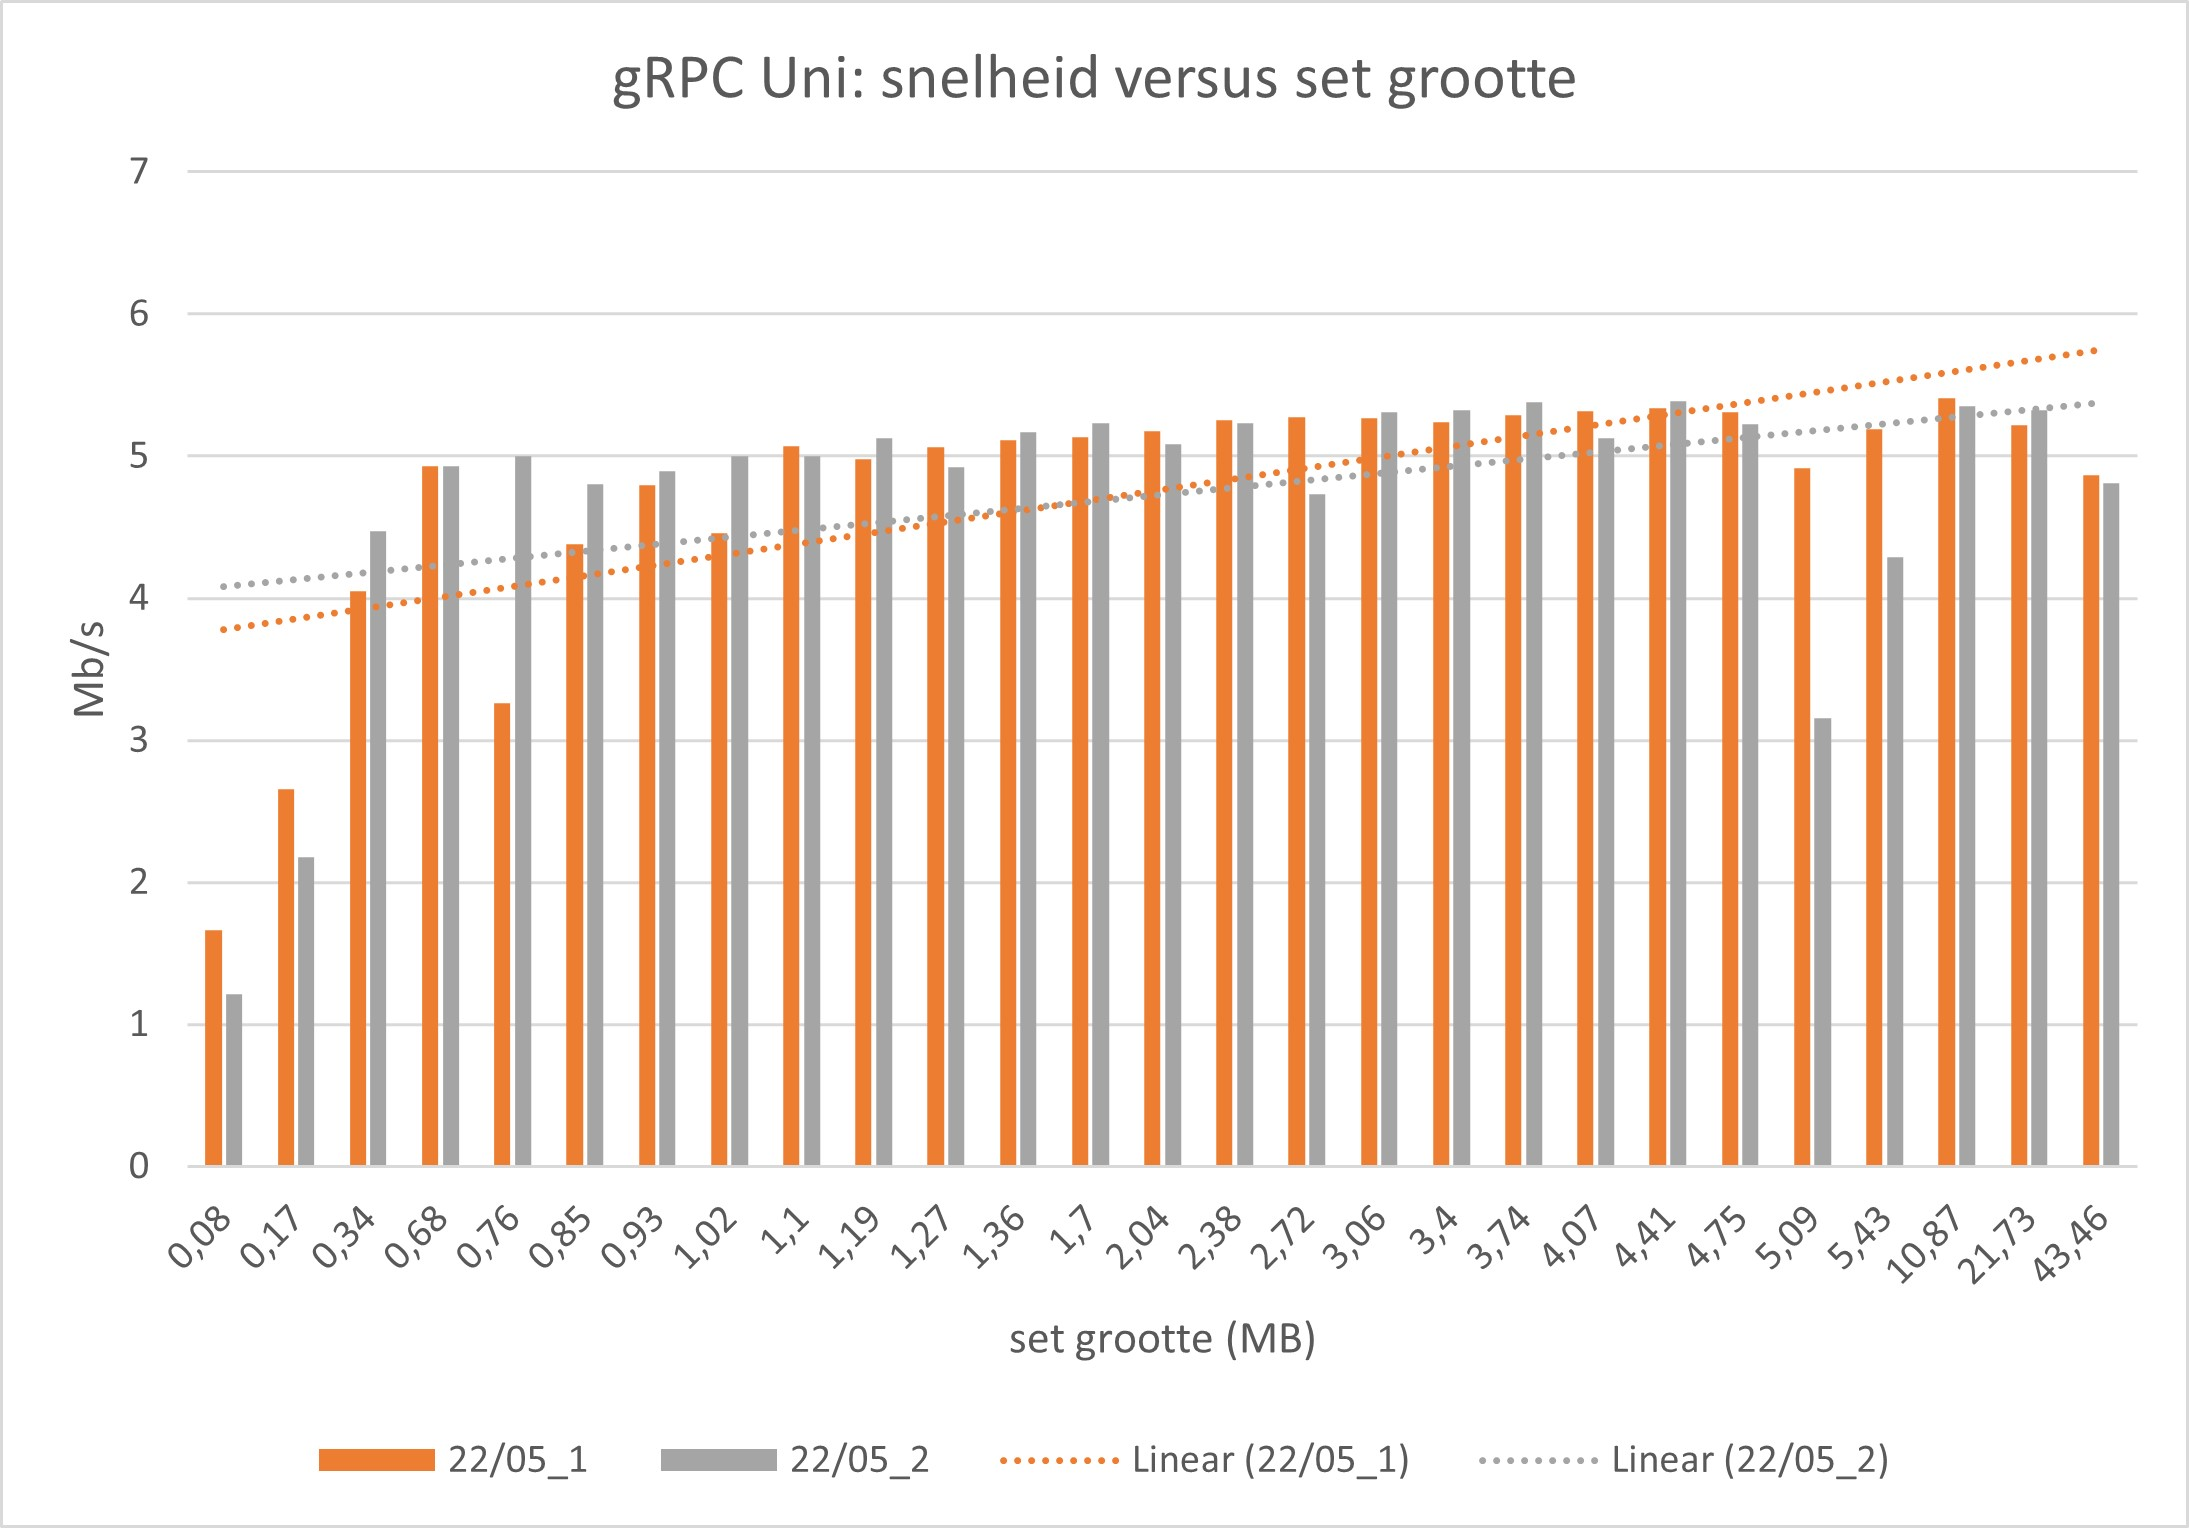
\includegraphics[width=1.0\linewidth]{gRPCUnienkelvoudigeRequests}
    \caption{[gRPC Uni enkelvoudige requests snelheid vs. grootte dataset]gRPC enkelvoudige requests snelheid vs. datasets van vari\"erende grootte}
    \label{fig:gRPCUnienkelvoudigeRequestsFig}
\end{figure}

De resultaten van de performantie testen voor de requests met de gRPC API functie getPeopleStream, welke een object van het type Multi teruggeeft zijn
terug te vinden in tabel ~\ref{tab:gRPCMultienkelvoudigtabel}.
Op figuur ~\ref{fig:gRPCMultienkelvoudigeRequestsFig} wordt de snelheid \(MB/sec\) weergegeven ten opzichte van de grootte van de dataset. Hier werd tevens een trendlijn voorzien.

\begin{table}
    \centering
    \begin{tabular}{llllll}
        \toprule
        \textbf{} & \textbf{} & \textbf{22/05/2023} & \textbf{} & \textbf{22/05/2023} & \textbf{} \\
        \midrule
        Groote subset (KB) & Groote subset (MB) & tijdsverloop (millies) & snelheid (Mb/s) & tijdsverloop (millies) & snelheid (Mb/s) \\
        86,94 & 0,08 & 41 & 1,951219512 & 45 & 1,777777778 \\
        173,89 & 0,17 & 52 & 3,269230769 & 68 & 2,5 \\
        347,76 & 0,34 & 88 & 3,863636364 & 89 & 3,820224719 \\
        695,53 & 0,68 & 164 & 4,146341463 & 163 & 4,171779141 \\
        782,43 & 0,76 & 180 & 4,222222222 & 184 & 4,130434783 \\
        869,26 & 0,85 & 231 & 3,67965368 & 214 & 3,971962617 \\
        956,19 & 0,93 & 216 & 4,305555556 & 219 & 4,246575342 \\
        1043,15 & 1,02 & 236 & 4,322033898 & 262 & 3,893129771 \\
        1130 & 1,1 & 252 & 4,365079365 & 259 & 4,247104247 \\
        1217,08 & 1,19 & 276 & 4,311594203 & 285 & 4,175438596 \\
        1303,88 & 1,27 & 293 & 4,33447099 & 295 & 4,305084746 \\
        1390,78 & 1,36 & 303 & 4,488448845 & 313 & 4,345047923 \\
        1738,59 & 1,7 & 374 & 4,545454545 & 399 & 4,260651629 \\
        2086,52 & 2,04 & 446 & 4,573991031 & 477 & 4,27672956 \\
        2434,17 & 2,38 & 526 & 4,524714829 & 538 & 4,423791822 \\
        2781,54 & 2,72 & 595 & 4,571428571 & 600 & 4,533333333 \\
        3129,44 & 3,06 & 658 & 4,650455927 & 674 & 4,540059347 \\
        3477,17 & 3,4 & 736 & 4,619565217 & 747 & 4,551539491 \\
        3824,75 & 3,74 & 802 & 4,663341646 & 846 & 4,420803783 \\
        4172,43 & 4,07 & 871 & 4,672789897 & 922 & 4,414316703 \\
        4520,25 & 4,41 & 954 & 4,622641509 & 966 & 4,565217391 \\
        4867,8 & 4,75 & 1011 & 4,698318497 & 1039 & 4,571703561 \\
        5216,06 & 5,09 & 1083 & 4,699907664 & 1131 & 4,500442087 \\
        5563,54 & 5,43 & 1177 & 4,613423959 & 1201 & 4,521232306 \\
        11126,99 & 10,87 & 2313 & 4,699524427 & 2358 & 4,609838846 \\
        22253,96 & 21,73 & 4616 & 4,707538995 & 4739 & 4,58535556 \\
        44507,32 & 43,46 & 9202 & 4,722886329 & 9291 & 4,677645033 \\
         &  &  &  &  &  \\
         & gemiddelde: &  & 4,327609997 &  & 4,186563708 \\
         & max: &  & 4,722886329 &  & 4,677645033 \\
         & min: &  & 1,951219512 &  & 1,777777778 \\
        \bottomrule
    \end{tabular}
    \caption{gRPC Multi}
    \label{tab:gRPCMultienkelvoudigtabel}
\end{table}

\begin{figure}[ht]
    \centering
    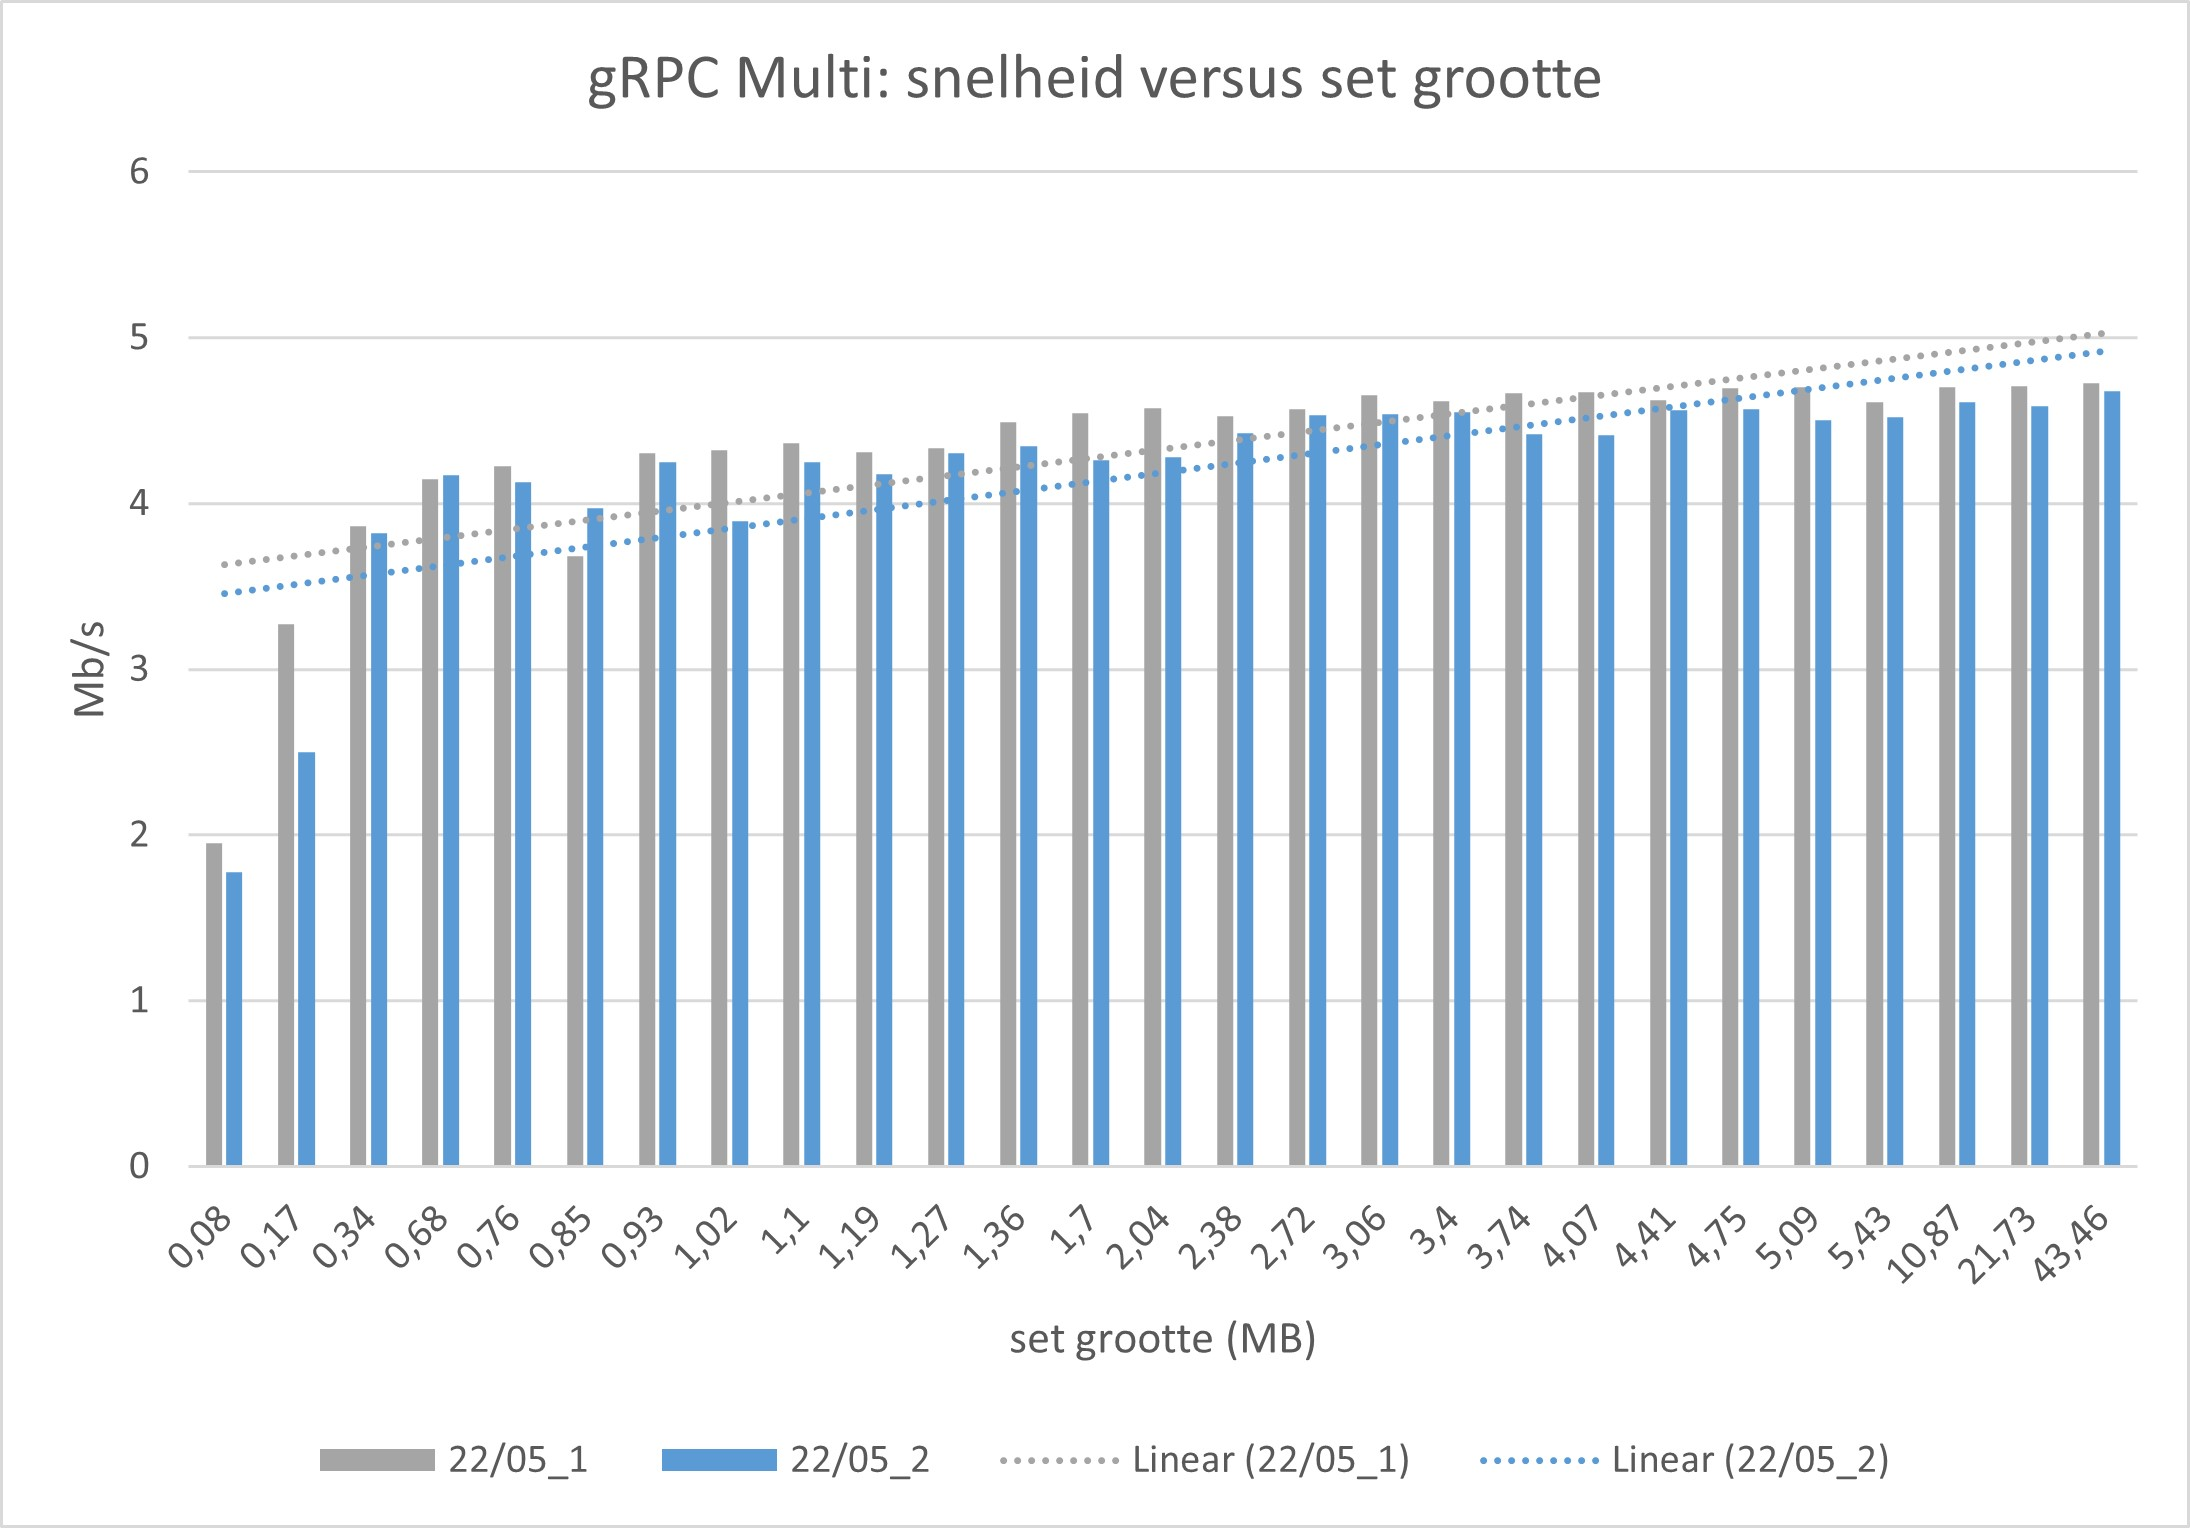
\includegraphics[width=1.0\linewidth]{gRPCMultienkelvoudigeRequests}
    \caption{[gRPC Multi snelheid vs. grootte dataset]gRPC Multi \(vgl. met enkelvoudige requests\) snelheid vs. datasets van vari\"erende grootte}
    \label{fig:gRPCMultienkelvoudigeRequestsFig}
\end{figure}

\section{Meervoudige requests}

% Voeg hier je eigen hoofdstukken toe die de ``corpus'' van je bachelorproef
% vormen. De structuur en titels hangen af van je eigen onderzoek. Je kan bv.
% elke fase in je onderzoek in een apart hoofdstuk bespreken.

%\input{...}
%\input{...}
%...

%%=============================================================================
%% Conclusie
%%=============================================================================

\chapter{Conclusie}%
\label{ch:conclusie}

\section{Bevindingen}
\paragraph{Enkelvoudige requests}
\textbf{REST - geen compressie}\newline
Zoals in hoofdstuk~\ref{ch:methodologie} voorgesteld werden de performantie testen voor de enkelvoudige requests, voor de voorgestelde dataset,
viermaal uitgevoerd en werd daarvan het gemiddelde genomen. Het resultaat is terug te vinden in tabel~\ref{tab:RESTenkelvoudig}.
Elke lijn op deze tabel komt overeen met een uitgevoerde request. In de eerste kolom worden het aantal items die werden opgevraagd weergegeven,
in de tweede kolom de grootte van de dataset, in MB, wanneer ze in JSON formaat naar een file worden weggeschreven,
daarna het tijdsverloop tussen de start van de request en het verkrijgen van de opgevraagde data in millieseconden. De laatste kolom geeft de de grootte van de
verzonden dataset, in MB, per seconde dat de request heeft geduurd.
Op figuur~\ref{fig:RESTenkelvoudig} wordt de snelheid, in MB/sec, weergegeven ten opzichte van de grootte van de verzonden dataset voor de vier sets van
calls die uitgevoerd werden, tevens werden trendlijnen voorzien volgens voortschrijdend gemiddelde over 3 metingen.\\

\begin{table}
    \centering
    \begin{tabular}{llll}
        \toprule
        \textbf{REST} & {Gemiddelde over 4 sets} & & \\
        \midrule
        Items / call & Grootte set (MB) & tijdsverloop (millies) & snelheid (Mb/s) \\
        1024 & 0,08 & 84,75 & 0,944 \\
        2048 & 0,17 & 136,25 & 1,248 \\
        4096 & 0,34 & 225,75 & 1,506 \\
        8192 & 0,68 & 438,5 & 1,551 \\
        9216 & 0,76 & 501,5 & 1,515 \\
        10240 & 0,85 & 546,25 & 1,556 \\
        11264 & 0,93 & 602,75 & 1,543 \\
        12288 & 1,02 & 644,5 & 1,583 \\
        13312 & 1,1 & 690,75 & 1,592 \\
        14336 & 1,19 & 742,25 & 1,603 \\
        15360 & 1,27 & 807,25 & 1,573 \\
        16384 & 1,36 & 857,5 & 1,586 \\
        20480 & 1,7 & 1057 & 1,608 \\
        24576 & 2,04 & 1277,5 & 1,597 \\
        28672 & 2,38 & 1468,75 & 1,620 \\
        32768 & 2,72 & 1676,5 & 1,622 \\
        36864 & 3,06 & 1894 & 1,616 \\
        40960 & 3,4 & 2104,5 & 1,616 \\
        45056 & 3,74 & 2309,75 & 1,619 \\
        49152 & 4,07 & 2546,5 & 1,598 \\
        53248 & 4,41 & 2753,5 & 1,602 \\
        57344 & 4,75 & 3208,5 & 1,480 \\
        61440 & 5,09 & 3165,5 & 1,608 \\
        65536 & 5,43 & 3347,5 & 1,622 \\
        131072 & 10,87 & 6759,5 & 1,608 \\
        262144 & 21,73 & 13689,75 & 1,587 \\
        524288 & 43,46 & 27022,25 & 1,608 \\
         &  &  &  \\
        gemiddelde: &  &  & 1,549 \\
        max: &  &  & 1,622 \\
        min: &  &  & 0,944 \\
        \bottomrule
    \end{tabular}
    \caption{REST - enkelvoudige requests: snelheid vs. datasets van vari\"erende grootte (gemiddelde over 4 sets)}
    \label{tab:RESTenkelvoudig}
\end{table}

\begin{figure}[ht]
    \centering
    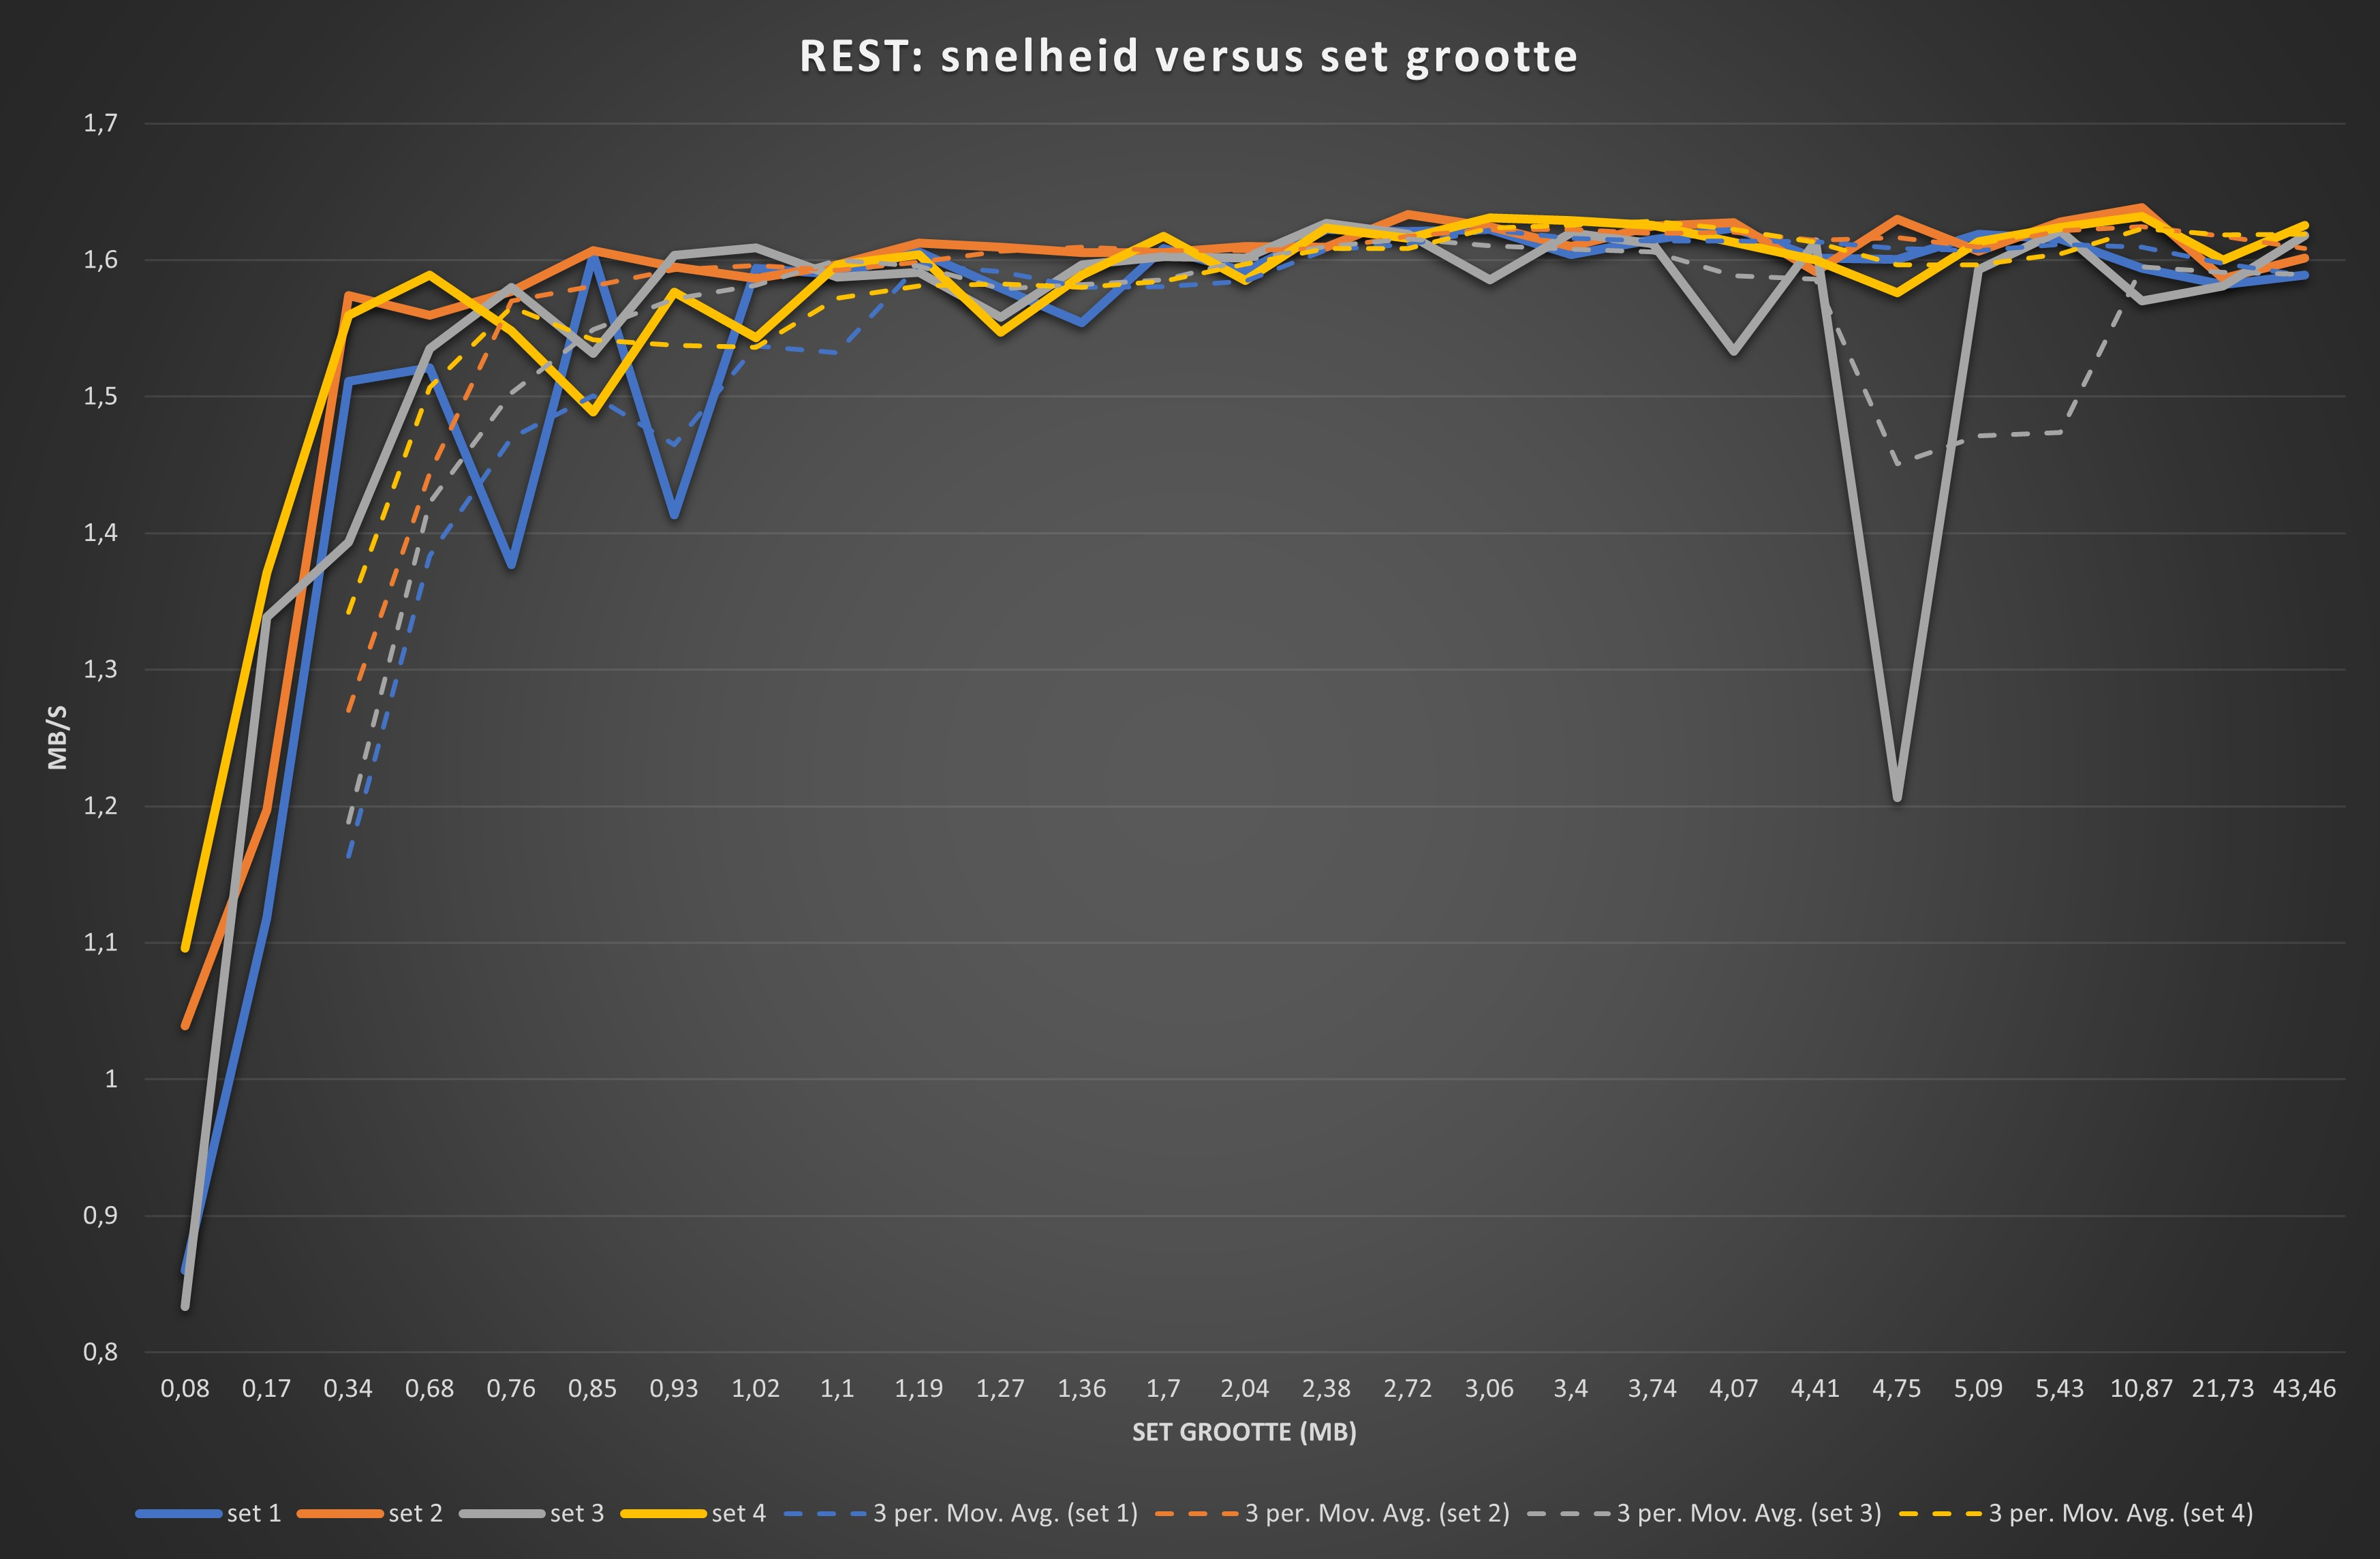
\includegraphics[width=1.0\linewidth]{REST_singular}
    \caption{REST - enkelvoudige requests: snelheid vs. datasets van vari\"erende grootte}
    \label{fig:RESTenkelvoudig}
\end{figure}

\textbf{REST - met compressie}\newline
De gemiddelden van de performantiemetingen van de enkelvoudige requests met het REST API waarbij de data door de server gecomprimeerd werd alvorens te verzenden
en bij de client weer is gedecomprimeerd, is terug te vinden in tabel~\ref{tab:RESTcompressieenkelvoudig}
Op figuur~\ref{fig:RESTcompressieenkelvoudig} wordt de snelheid, in MB/sec, weergegeven ten opzichte van de grootte van de verzonden dataset voor de vier sets van
calls die uitgevoerd werden, tevens werden trendlijnen voorzien volgens voortschrijdend gemiddelde over 3 metingen.\\

\begin{table}
    \centering
    \begin{tabular}{llll}
        \toprule
        \textbf{REST gecomprimeerd} & {Gemiddelde over 4 sets} &  & \\
        \midrule
        Items / call & Grootte set (MB) & tijdsverloop (millies) & snelheid (MB/s) \\
        1024 & 0,08 & 84,75 & 0,944 \\
        2048 & 0,17 & 85,25 & 1,994 \\
        4096 & 0,34 & 99,5 & 3,417 \\
        8192 & 0,68 & 151,5 & 4,488 \\
        9216 & 0,76 & 201 & 3,781 \\
        10240 & 0,85 & 208,25 & 4,082 \\
        11264 & 0,93 & 216,25 & 4,301 \\
        12288 & 1,02 & 230 & 4,435 \\
        13312 & 1,1 & 214 & 5,140 \\
        14336 & 1,19 & 245 & 4,857 \\
        15360 & 1,27 & 240,5 & 5,281 \\
        16384 & 1,36 & 255,25 & 5,328 \\
        20480 & 1,7 & 316 & 5,380 \\
        24576 & 2,04 & 371,75 & 5,488 \\
        28672 & 2,38 & 442,5 & 5,379 \\
        32768 & 2,72 & 488,25 & 5,571 \\
        36864 & 3,06 & 554 & 5,523 \\
        40960 & 3,4 & 593,25 & 5,731 \\
        45056 & 3,74 & 665,25 & 5,622 \\
        49152 & 4,07 & 734,25 & 5,543 \\
        53248 & 4,41 & 860,25 & 5,126 \\
        57344 & 4,75 & 960,25 & 4,947 \\
        61440 & 5,09 & 1003,5 & 5,072 \\
        65536 & 5,43 & 1164,25 & 4,664 \\
        131072 & 10,87 & 2079,75 & 5,227 \\
        262144 & 21,73 & 3909 & 5,559 \\
        524288 & 43,46 & 8374,25 & 5,190 \\
         &  &  &  \\
        gemiddelde: &  &  & 4,743 \\
        max: &  &  & 5,731 \\
        min: &  &  & 0,944 \\
        \bottomrule
    \end{tabular}
    \caption{REST gecomprimeerd  - enkelvoudige requests: snelheid vs. datasets van vari\"erende grootte (gemiddelde over 4 sets)}
    \label{tab:RESTcompressieenkelvoudig}
\end{table}


\begin{figure}[ht]
    \centering
    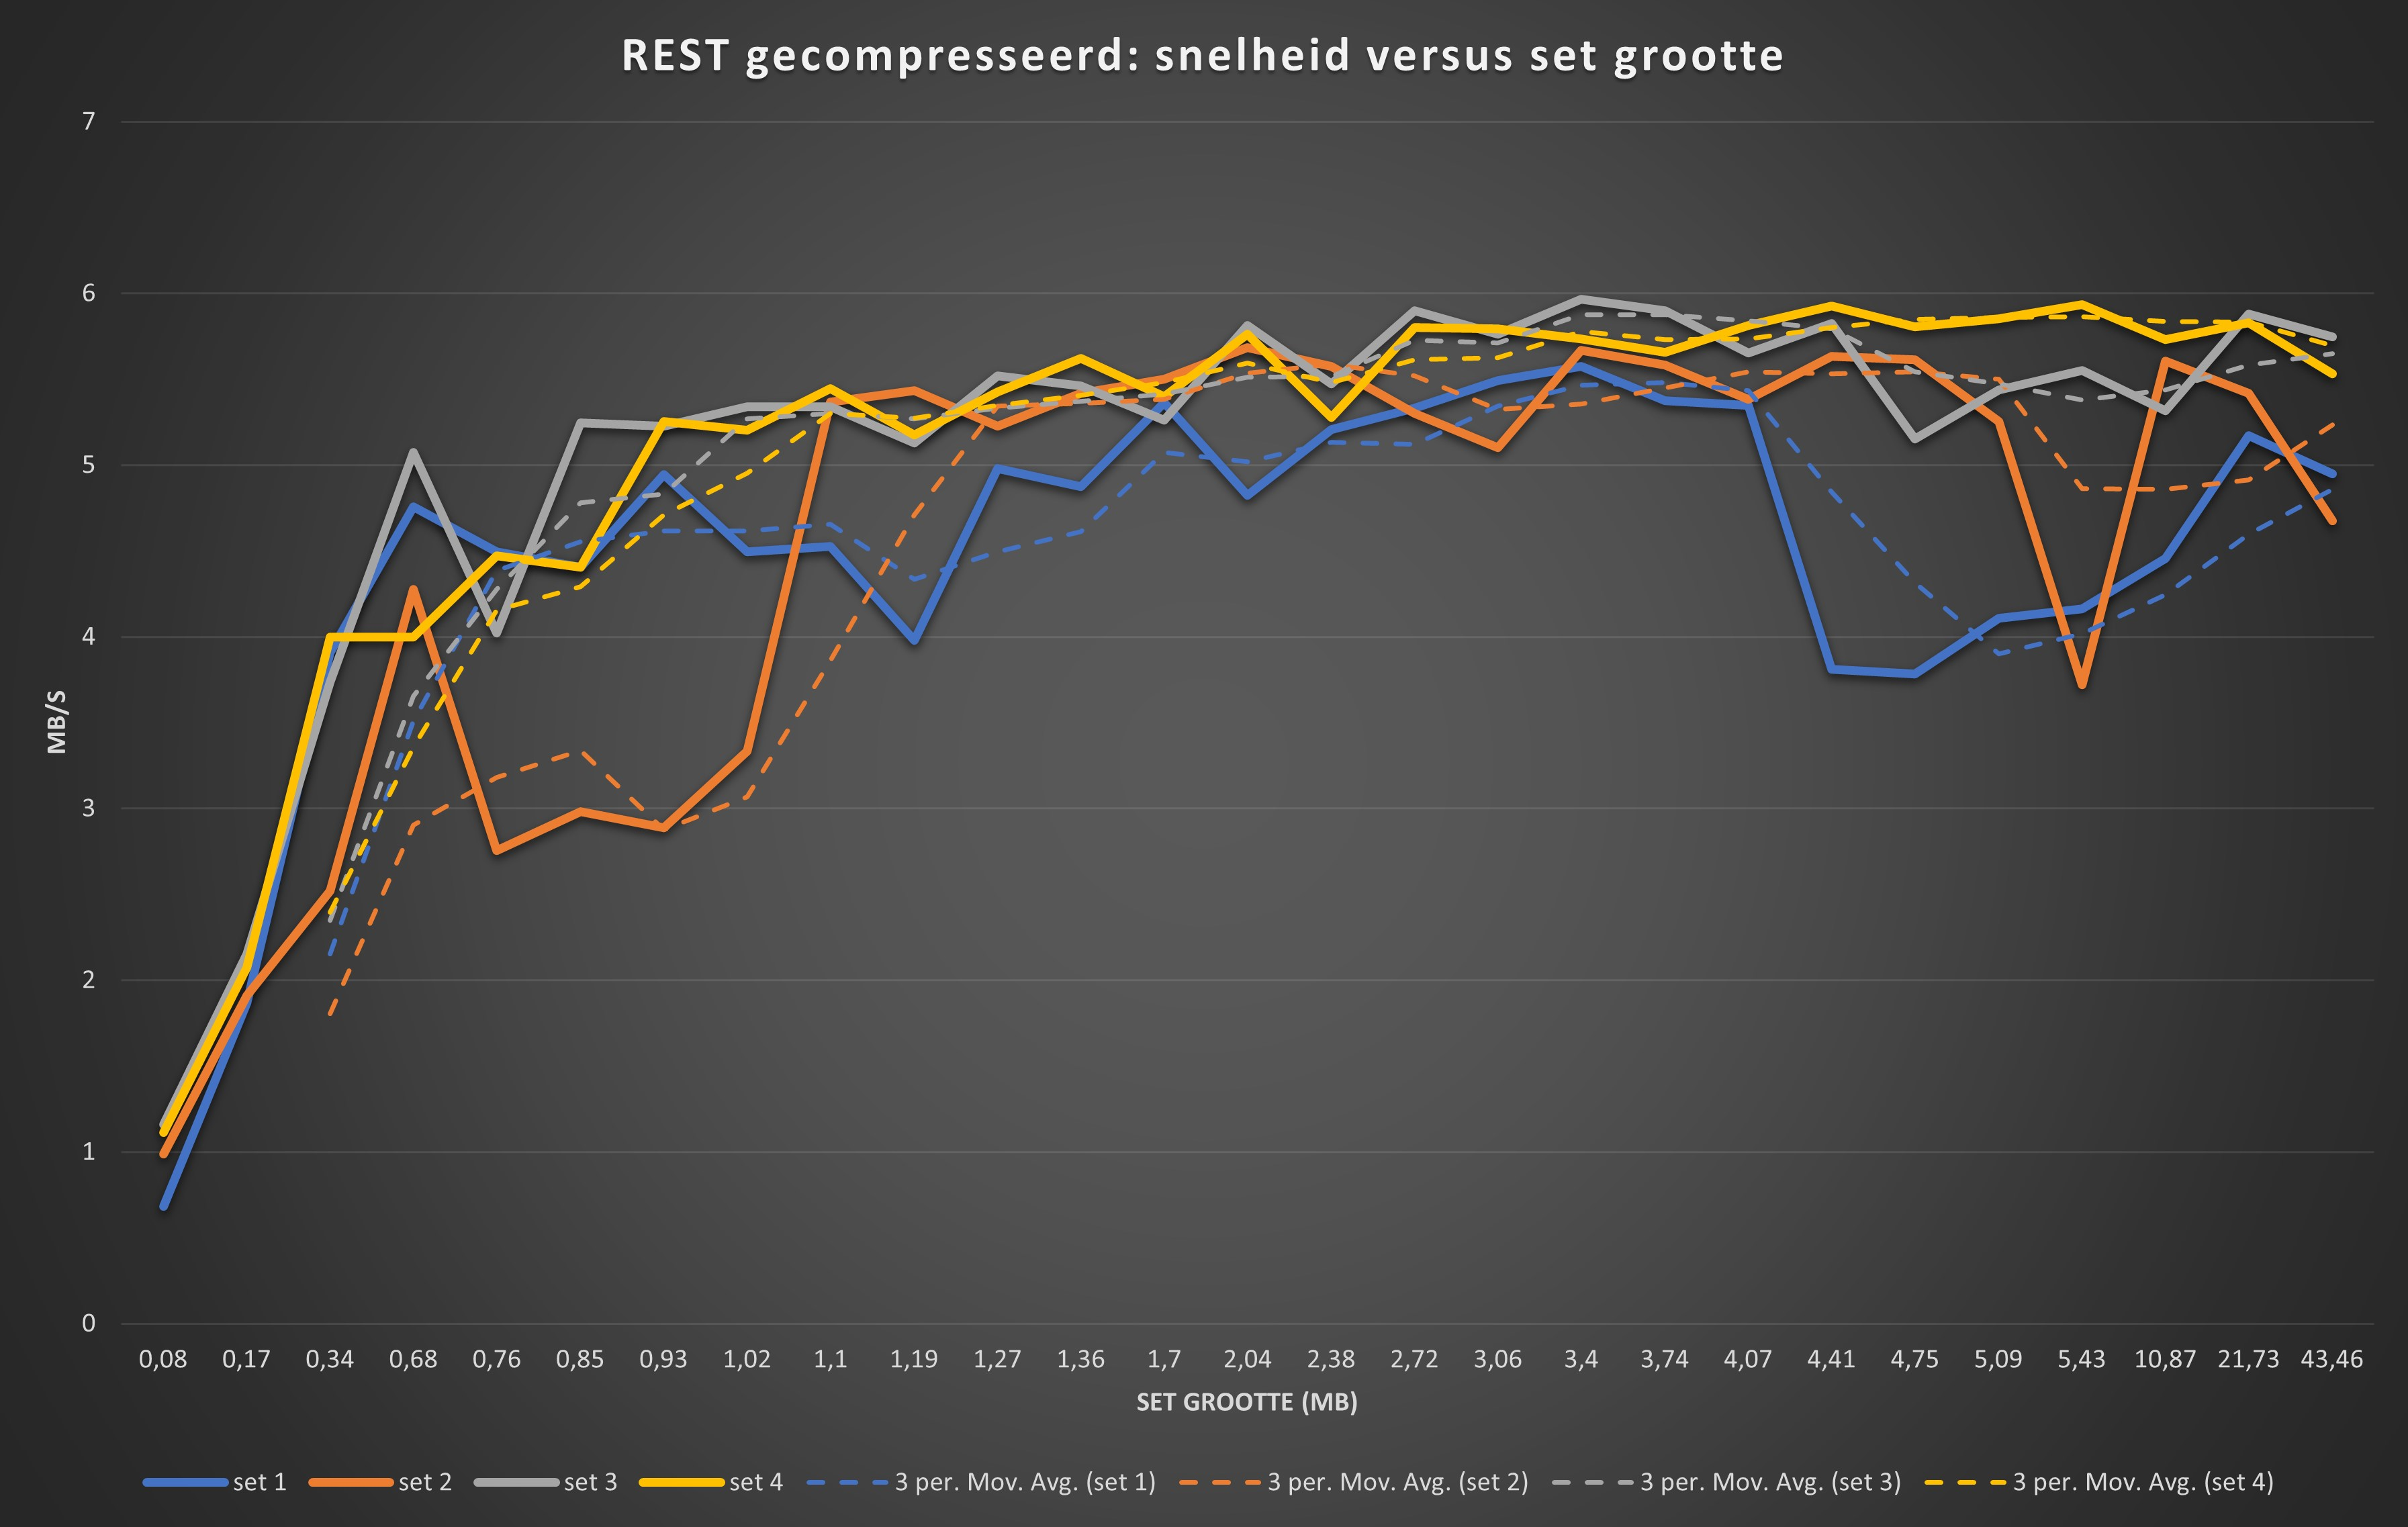
\includegraphics[width=1.0\linewidth]{REST_compressed_singular}
    \caption{REST gecomprimeerd - enkelvoudige requests: snelheid vs. datasets van vari\"erende grootte}
    \label{fig:RESTcompressieenkelvoudig}
\end{figure}

\textbf{gRPC - Uni}\newline
De gemiddelden van de performantiemeting van de enkelvoudige requests met de gRPC API functie getPeople, welke een object van het type Uni teruggeeft, zijn
terug te vinden in tabel~\ref{tab:gRPCUnienkelvoudig}
Op figuur~\ref{fig:RESTcompressieenkelvoudig} wordt de snelheid in MB/sec weergegeven ten opzichte van de grootte van de verzonden dataset voor de vier sets van
calls die uitgevoerd werden. Tevens werden trendlijnen voorzien volgens voortschrijdend gemiddelde over 3 metingen.\\
Op figuur~\ref{fig:gRPCUnienkelvoudig} wordt de snelheid, in MB/sec, weergegeven ten opzichte van de grootte van de verzonden dataset voor de vier sets van
calls die uitgevoerd werden. Ook hier werden trendlijnen voorzien volgens voortschrijdend gemiddelde over 3 metingen.\\

\begin{table}
    \centering
    \begin{tabular}{llll}
        \toprule
        \textbf{gRPC Uni} & {Gemiddelde over 4 sets} &  & \\
        \midrule
        Items / call & Groote subset (MB) & tijdsverloop (millies) & snelheid (MB/s) \\
        1024 & 0,08 & 47,25 & 1,693121693 \\
        2048 & 0,17 & 79,25 & 2,14511041 \\
        4096 & 0,34 & 85 & 4 \\
        8192 & 0,68 & 142,5 & 4,771929825 \\
        9216 & 0,76 & 159,5 & 4,764890282 \\
        10240 & 0,85 & 182,5 & 4,657534247 \\
        11264 & 0,93 & 187,5 & 4,96 \\
        12288 & 1,02 & 217 & 4,700460829 \\
        13312 & 1,1 & 219 & 5,02283105 \\
        14336 & 1,19 & 238,5 & 4,98951782 \\
        15360 & 1,27 & 265,25 & 4,78793591 \\
        16384 & 1,36 & 268 & 5,074626866 \\
        20480 & 1,7 & 339 & 5,014749263 \\
        24576 & 2,04 & 407,5 & 5,006134969 \\
        28672 & 2,38 & 463,75 & 5,132075472 \\
        32768 & 2,72 & 526 & 5,171102662 \\
        36864 & 3,06 & 582,25 & 5,255474453 \\
        40960 & 3,4 & 647,25 & 5,252993434 \\
        45056 & 3,74 & 718,75 & 5,203478261 \\
        49152 & 4,07 & 763,5 & 5,330713818 \\
        53248 & 4,41 & 828 & 5,326086957 \\
        57344 & 4,75 & 892,25 & 5,323620062 \\
        61440 & 5,09 & 966,75 & 5,265063357 \\
        65536 & 5,43 & 1021 & 5,318315377 \\
        131072 & 10,87 & 2007,75 & 5,41402067 \\
        262144 & 21,73 & 4044,25 & 5,373060518 \\
        524288 & 43,46 & 8136 & 5,341691249 \\
         &  &  &  \\
        gemiddelde: &  &  & 4,825797757 \\
        max: &  &  & 5,41402067 \\
        min: &  &  & 1,693121693 \\
        \bottomrule
    \end{tabular}
    \caption{gRPC Uni - enkelvoudige requests: snelheid vs. datasets van vari\"erende grootte (gemiddelde over 4 sets)}
    \label{tab:gRPCUnienkelvoudig}
\end{table}


\begin{figure}[ht]
    \centering
    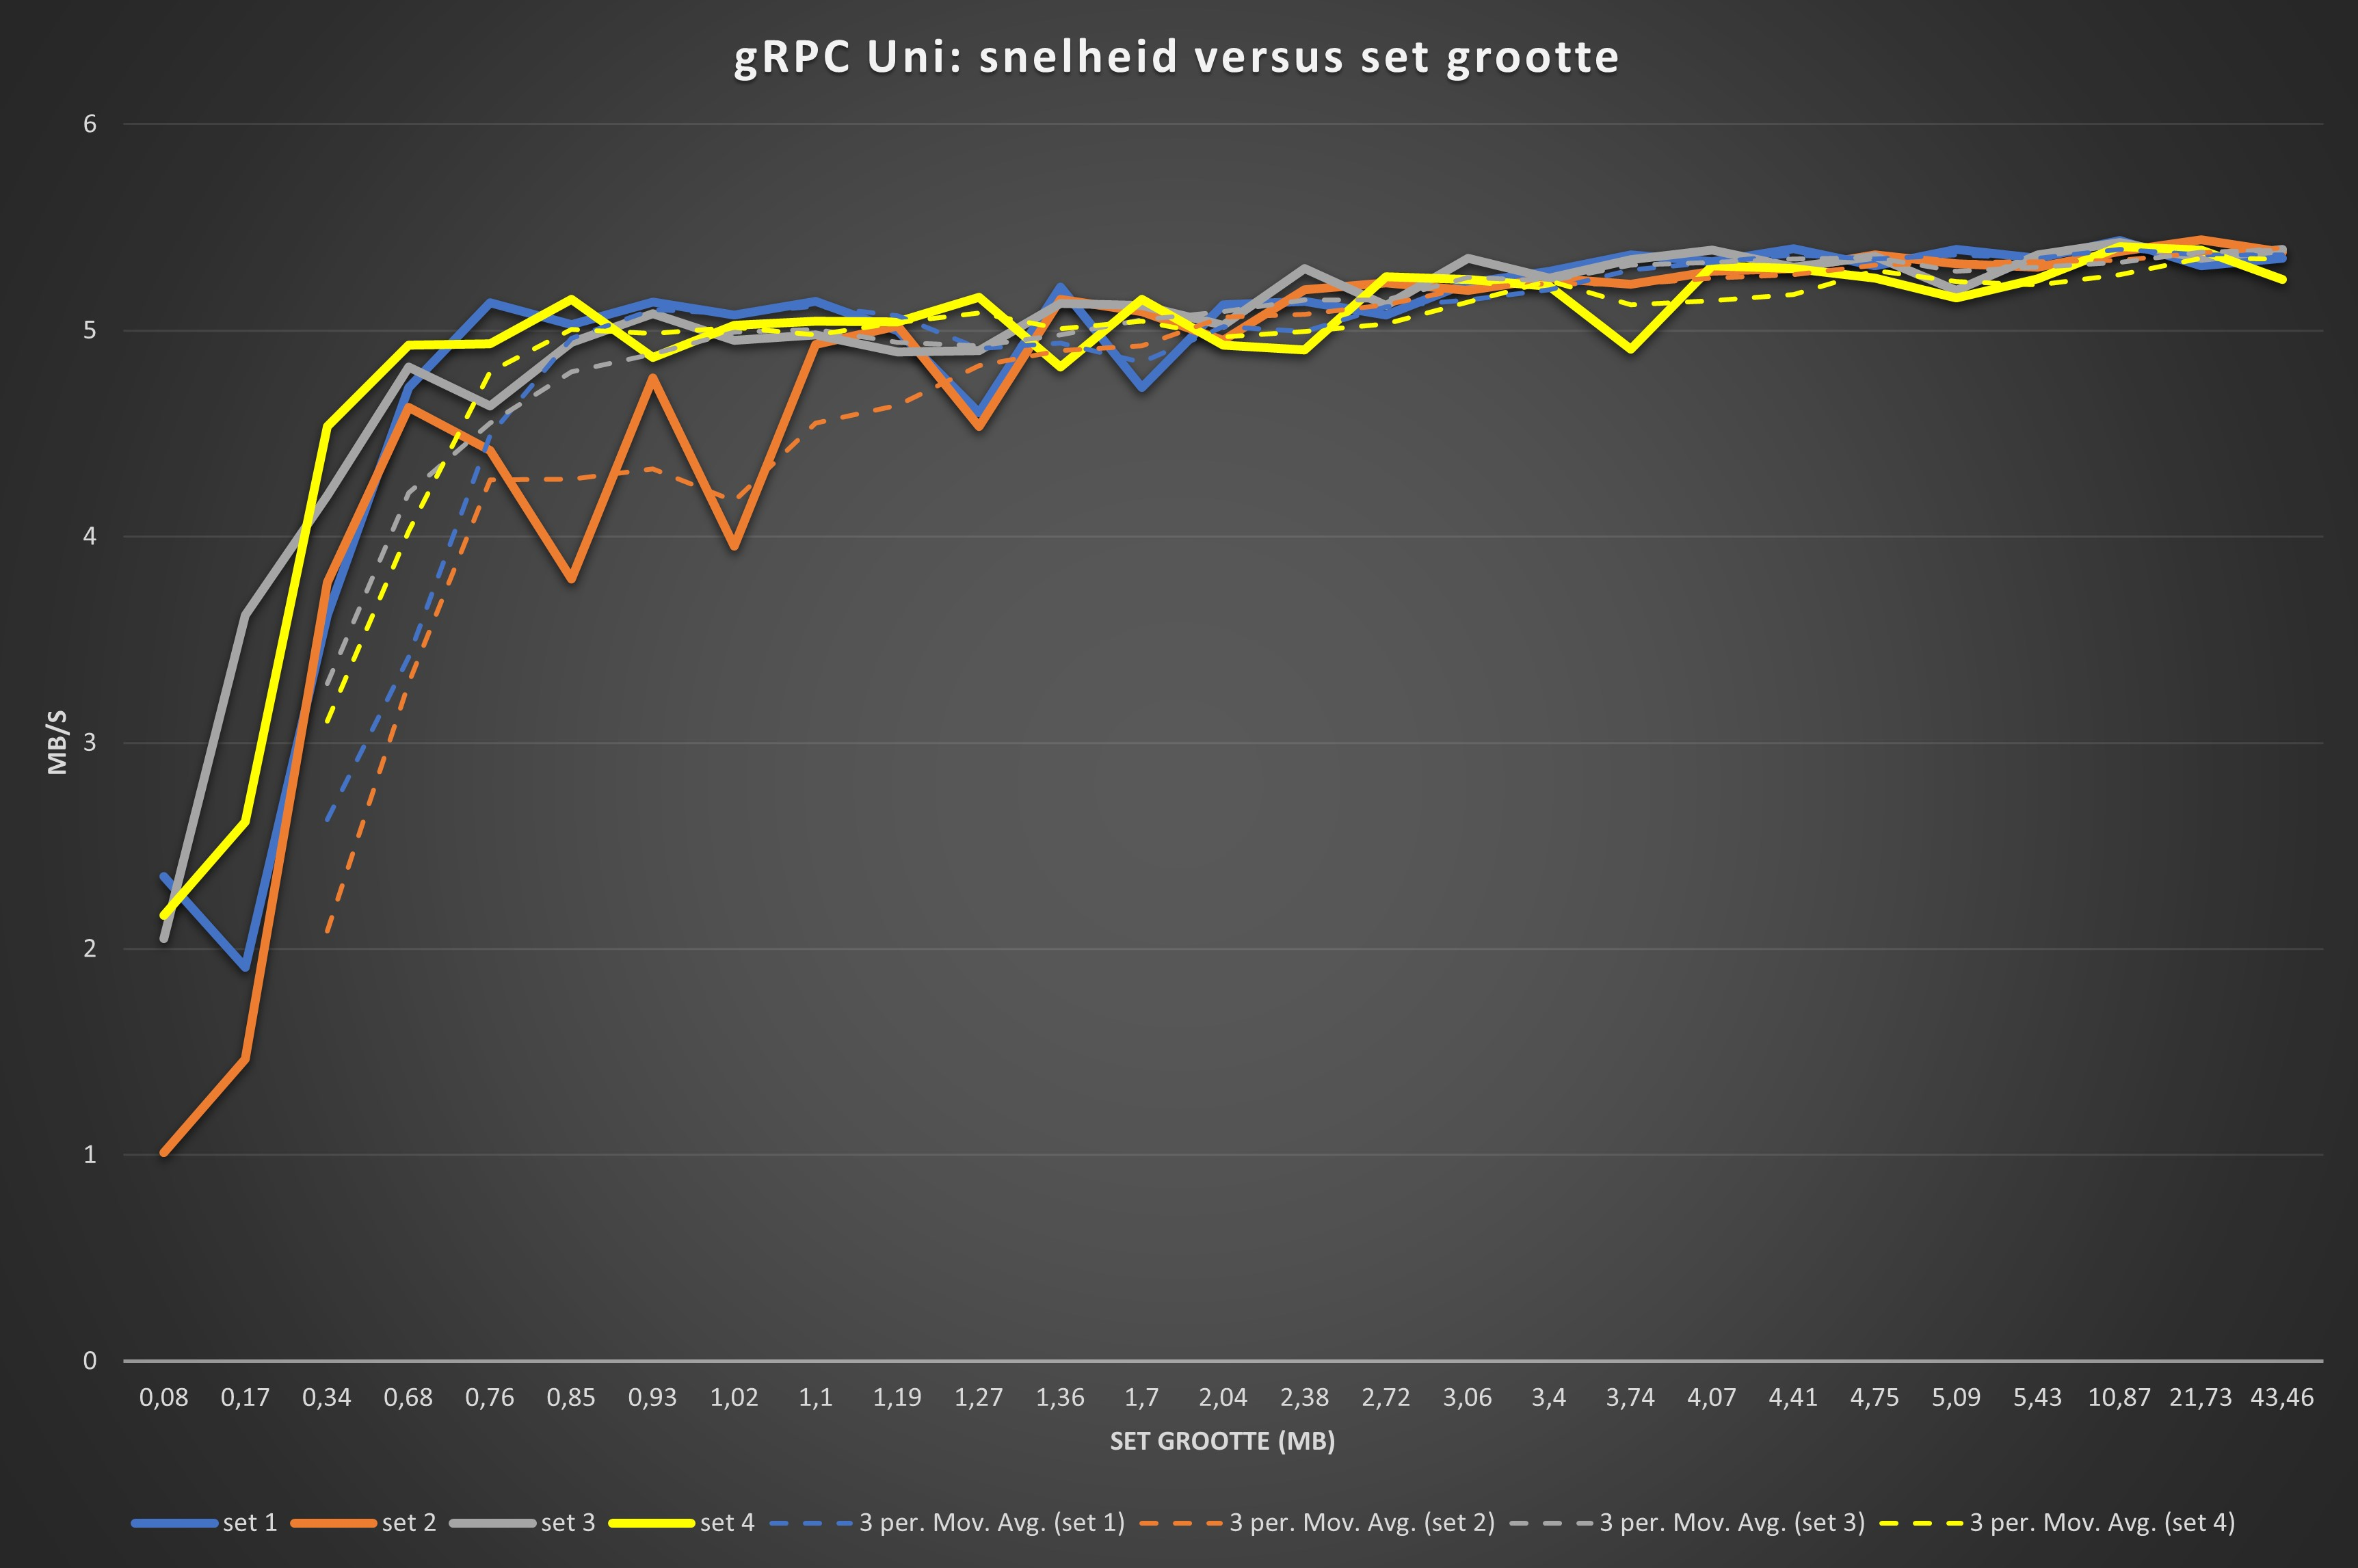
\includegraphics[width=1.0\linewidth]{gRPC_Uni_singular}
    \caption{gRPC Uni - enkelvoudige requests: snelheid vs. datasets van vari\"erende grootte}
    \label{fig:gRPCUnienkelvoudig}
\end{figure}

\textbf{gRPC - Multi}\newline
De gemiddelden van de performantiemetingen van de enkelvoudige requests met de gRPC API functie getPeopleStream, welke een object van het type Multi is, en daarmee een stream
teruggeeft, zijn terug te vinden in tabel~\ref{tab:gRPCMultienkelvoudig}
Op figuur~\ref{fig:gRPCMultienkelvoudig} wordt de snelheid in MB/sec weergegeven ten opzichte van de grootte van de verzonden dataset voor de vier sets van
calls die uitgevoerd werden. Tevens werden trendlijnen voorzien volgens voortschrijdend gemiddelde over 3 metingen.\\

\begin{table}
    \centering
    \begin{tabular}{llll}
        \toprule
        \textbf{gRPC Multi} & \textbf{Gemiddelde over 4 sets} & \textbf{aze} & \textbf{aze} \\
        \midrule
        Items / call & Groote subset (MB) & tijdsverloop (millies) & snelheid (MB/s) \\
        1024 & 0,08 & 41,5 & 1,927710843 \\
        2048 & 0,17 & 56 & 3,035714286 \\
        4096 & 0,34 & 90,25 & 3,767313019 \\
        8192 & 0,68 & 170,25 & 3,994126285 \\
        9216 & 0,76 & 187,25 & 4,058744993 \\
        10240 & 0,85 & 195 & 4,358974359 \\
        11264 & 0,93 & 217,5 & 4,275862069 \\
        12288 & 1,02 & 242,25 & 4,210526316 \\
        13312 & 1,1 & 259 & 4,247104247 \\
        14336 & 1,19 & 273,5 & 4,351005484 \\
        15360 & 1,27 & 294,5 & 4,312393888 \\
        16384 & 1,36 & 303,75 & 4,477366255 \\
        20480 & 1,7 & 383 & 4,438642298 \\
        24576 & 2,04 & 447,5 & 4,558659218 \\
        28672 & 2,38 & 525,75 & 4,526866381 \\
        32768 & 2,72 & 667,25 & 4,076433121 \\
        36864 & 3,06 & 671,25 & 4,558659218 \\
        40960 & 3,4 & 731 & 4,651162791 \\
        45056 & 3,74 & 807,75 & 4,630145466 \\
        49152 & 4,07 & 882,5 & 4,611898017 \\
        53248 & 4,41 & 964,25 & 4,573502722 \\
        57344 & 4,75 & 1042,75 & 4,555262527 \\
        61440 & 5,09 & 1106,75 & 4,599051276 \\
        65536 & 5,43 & 1168,25 & 4,647977744 \\
        131072 & 10,87 & 2356,5 & 4,612773181 \\
        262144 & 21,73 & 4727,5 & 4,596509783 \\
        524288 & 43,46 & 9285,25 & 4,680541719 \\
         &  &  &  \\
        gemiddelde: &  & 4,271663982 & null \\
        max: &  &  & 4,680541719 \\
        min: & 0 & 0 & 1,927710843 \\
        \bottomrule
    \end{tabular}
    \caption{gRPC Multi - enkelvoudige requests: snelheid vs. datasets van vari\"erende grootte (gemiddelde over 4 sets)}
    \label{tab:gRPCMultienkelvoudig}
\end{table}

\begin{figure}[ht]
    \centering
    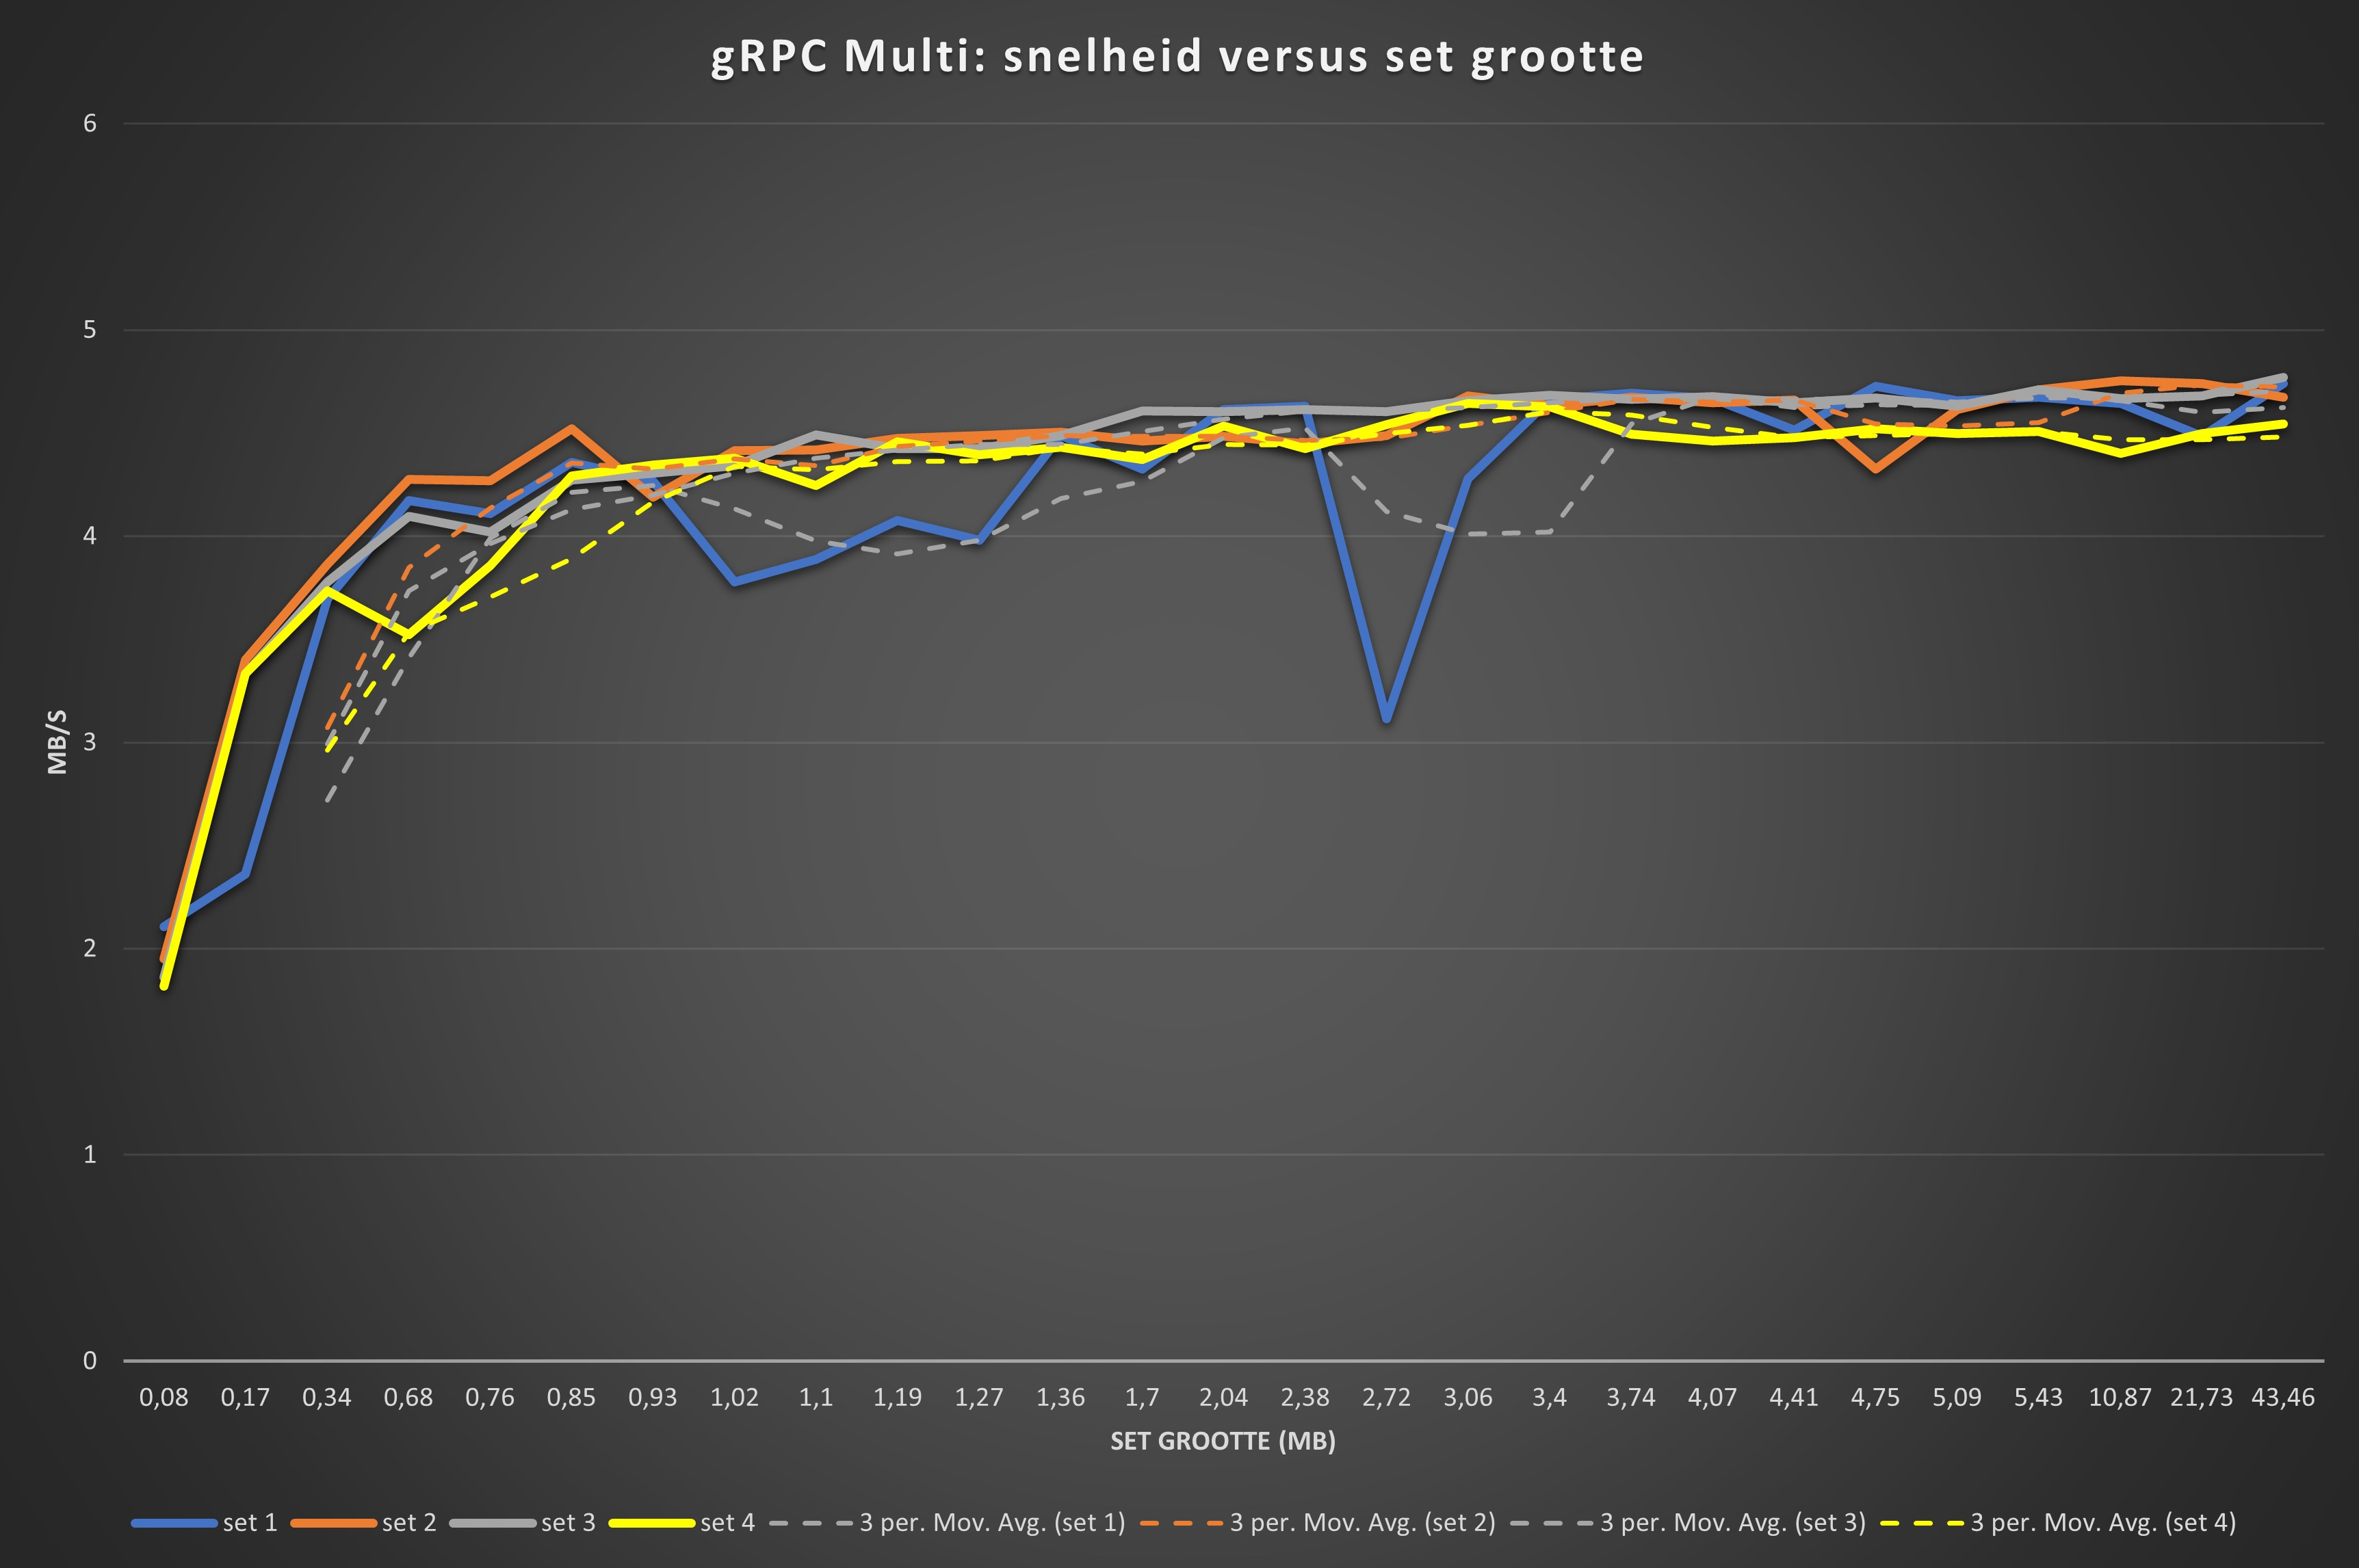
\includegraphics[width=1.0\linewidth]{gRPC_Multi_singular}
    \caption{gRPC Multi - enkelvoudige requests: snelheid vs. datasets van vari\"erende grootte}
    \label{fig:gRPCMultienkelvoudig}
\end{figure}

Tot slot worden de gemiddelde waarden, over de vier sets van calls, voor de vier verschillende types van call, samen in een grafiek geplaatst
welke wordt weergegeven in figuur~\ref{fig:RESTRESTcompressiegRPCUnigRPCMulti} alsook worden de gemiddelde tijdsduur per dataset per type call
als percentage weergegeven t.o.v. het tijdsverloop van de meest performante gemiddelde waarde in tabel~\ref{tab:REST_RESTcompressie_gRPCUni_gRPCMultipercentage}\\
\begin{figure}[ht]
    \centering
    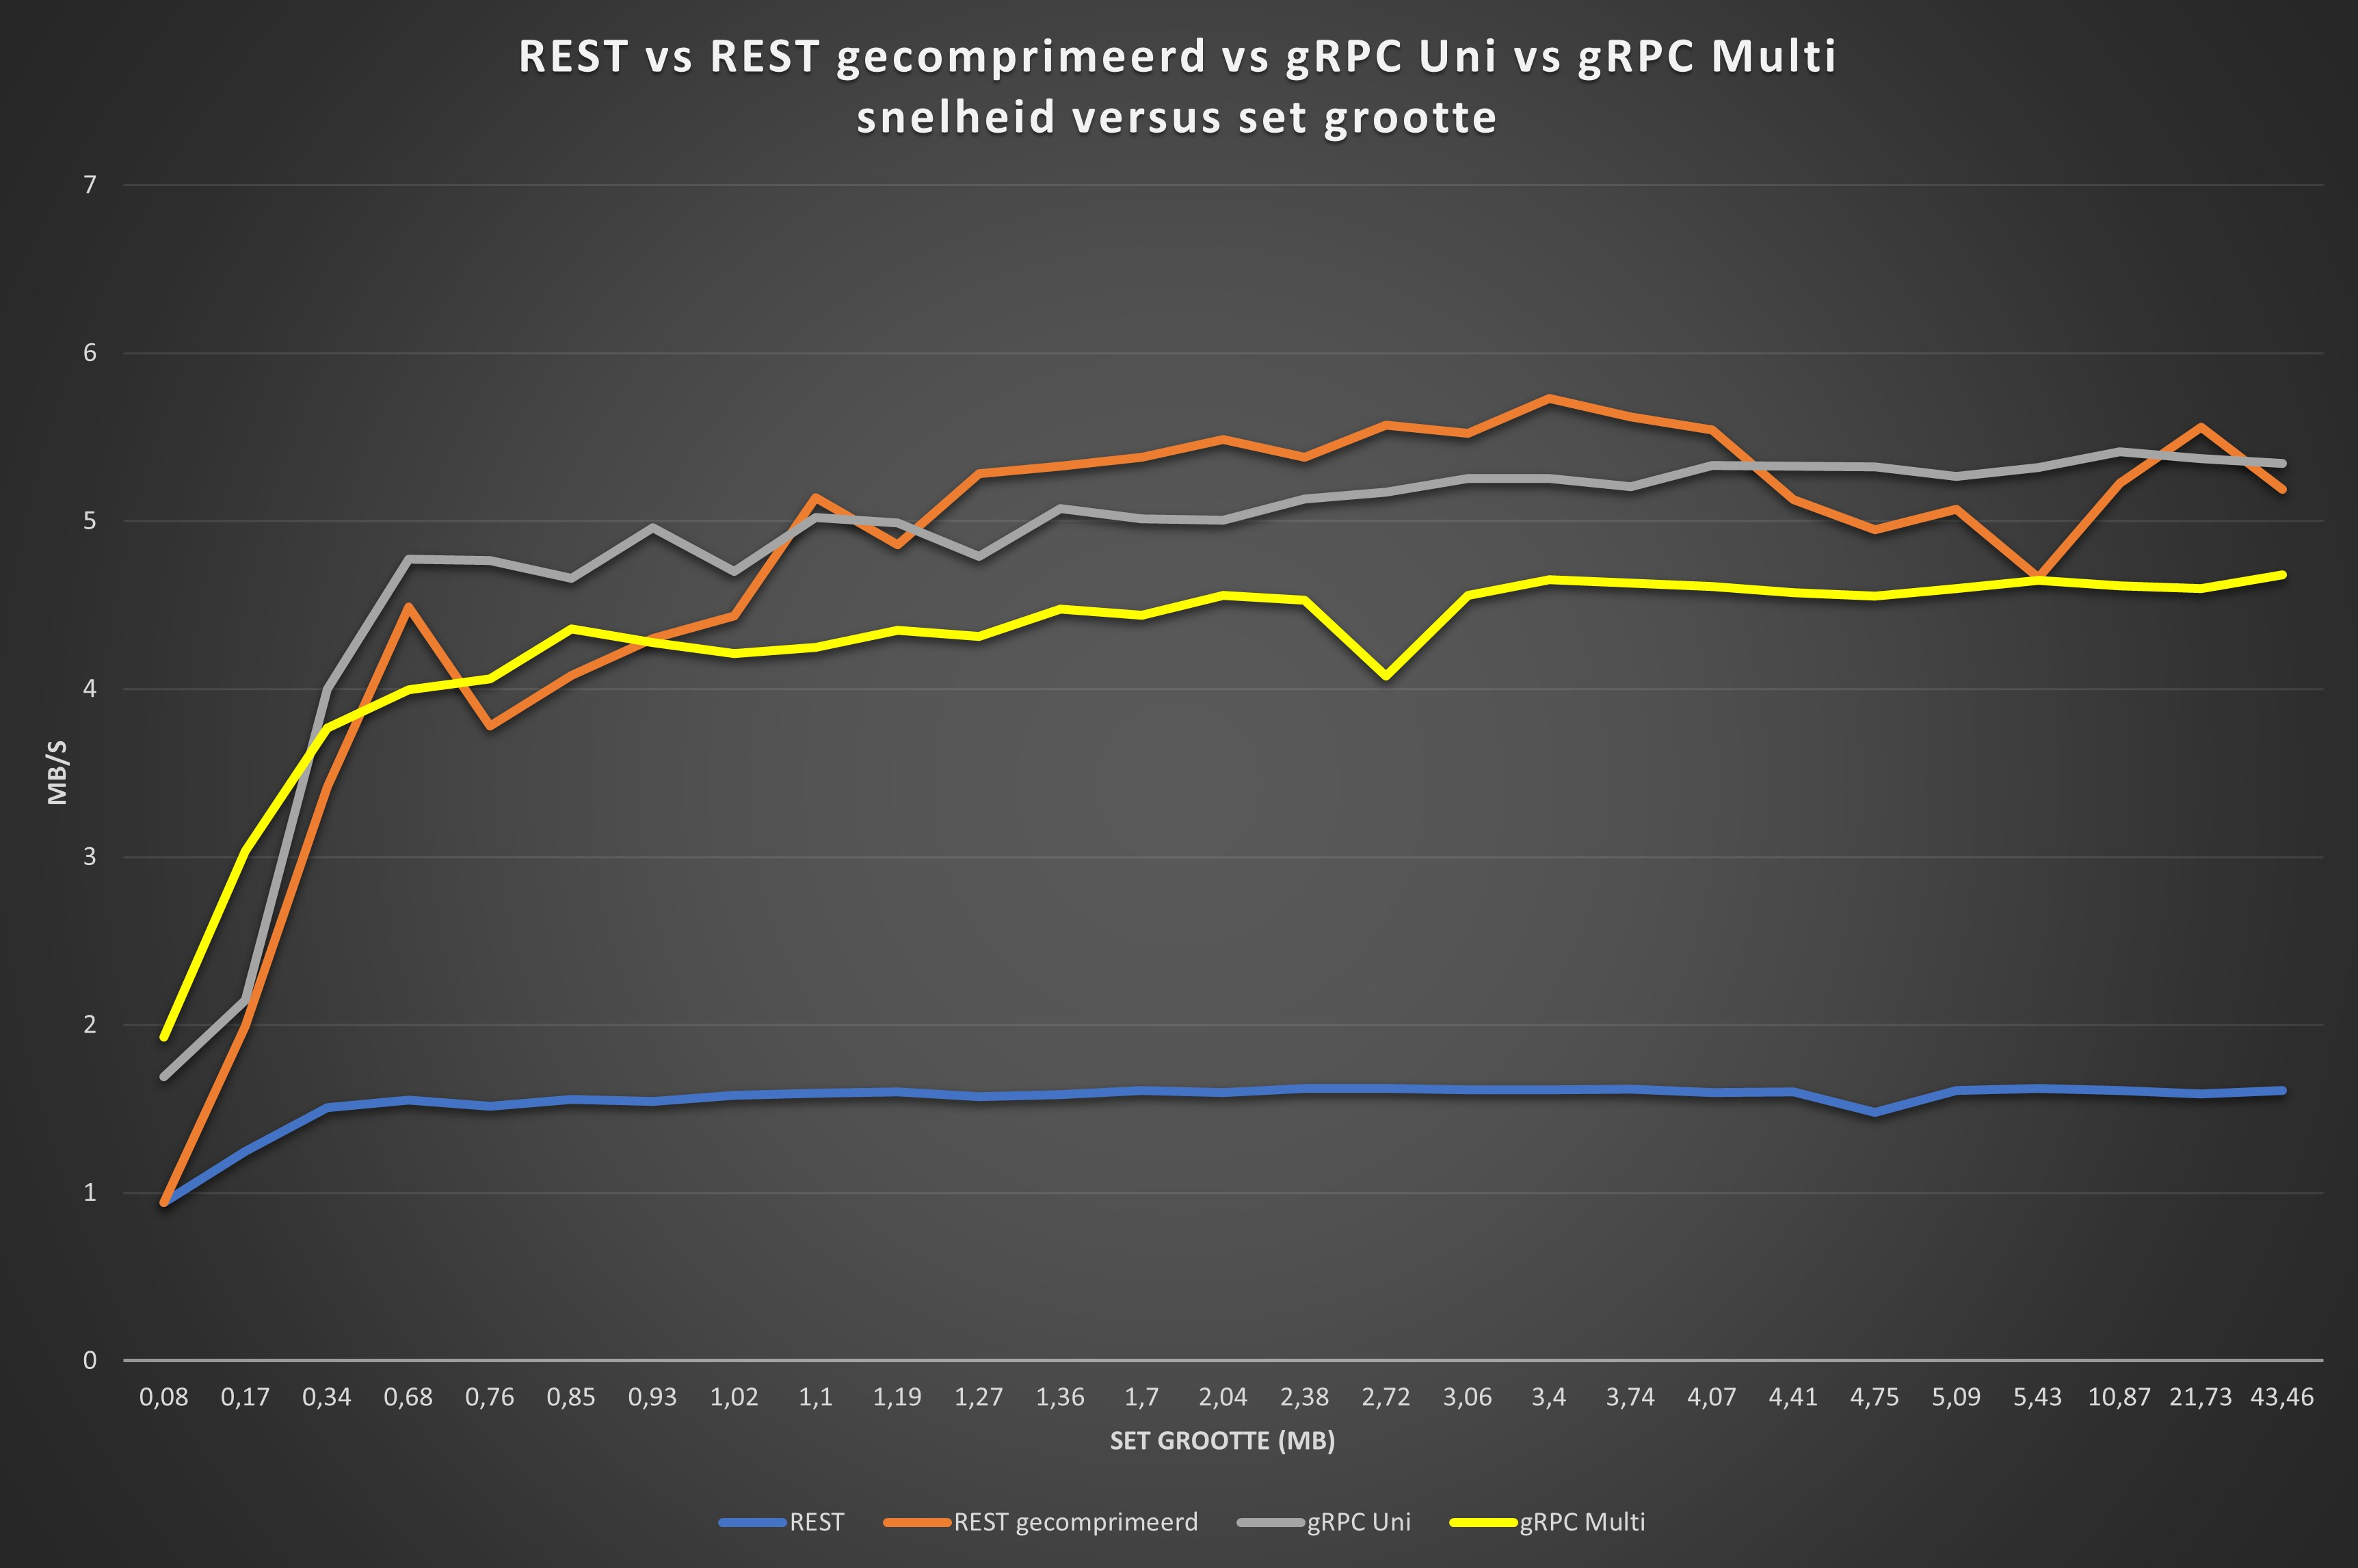
\includegraphics[width=1.0\linewidth]{REST_vs_REST_compressed_vs_gRPC_Uni_vs_gRPC_Multi_singular}
    \caption{REST vs REST met compressie vs gRPC Uni vs gRPC Multi - enkelvoudige requests: snelheid vs. datasets van vari\"erende grootte}
    \label{fig:RESTRESTcompressiegRPCUnigRPCMulti}
\end{figure}

\begin{table}
    \centering
    \begin{tabular}{lllll}
        \toprule
         & \textbf{REST} & \textbf{REST gecomprimeerd} & \textbf{gRPC Uni} & \textbf{gRPC Multi} \\
        \midrule
        Grootte set (MB) &  &  & \\
        0,08 & 204,22\% & 204,22\% & 113,86\% & \textbf{100,00}\% \\
        0,17 & 243,30\% & 152,23\% & 141,52\% & \textbf{100,00}\% \\
        0,34 & 265,59\% & 117,06\% & \textbf{100,00}\% & 106,18\% \\
        0,68 & 307,72\% & 106,32\% & \textbf{100,00}\% & 119,47\% \\
        0,76 & 314,42\% & 126,02\% & \textbf{100,00}\% & 117,40\% \\
        0,85 & 299,32\% & 114,11\% & \textbf{100,00}\% & 106,85\% \\
        0,93 & 321,47\% & 115,33\% & \textbf{100,00}\% & 116,00\% \\
        1,02 & 297,00\% & 105,99\% & \textbf{100,00}\% & 111,64\% \\
        1,1 & 322,78\% & \textbf{100,00}\% & 102,34\% & 121,03\% \\
        1,19 & 311,22\% & 102,73\% & \textbf{100,00}\% & 114,68\% \\
        1,27 & 335,65\% & \textbf{100,00}\% & 110,29\% & 122,45\% \\
        1,36 & 335,95\% & \textbf{100,00}\% & 105,00\% & 119,00\% \\
        1,7 & 334,49\% & \textbf{100,00}\% & 107,28\% & 121,20\% \\
        2,04 & 343,64\% & \textbf{100,00}\% & 109,62\% & 120,38\% \\
        2,38 & 331,92\% & \textbf{100,00}\% & 104,80\% & 118,81\% \\
        2,72 & 343,37\% & \textbf{100,00}\% & 107,73\% & 136,66\% \\
        3,06 & 341,88\% & \textbf{100,00}\% & 105,10\% & 121,16\% \\
        3,4 & 354,74\% & \textbf{100,00}\% & 109,10\% & 123,22\% \\
        3,74 & 347,20\% & \textbf{100,00}\% & 108,04\% & 121,42\% \\
        4,07 & 346,82\% & \textbf{100,00}\% & 103,98\% & 120,19\% \\
        4,41 & 332,55\% & 103,89\% & \textbf{100,00}\% & 116,46\% \\
        4,75 & 359,60\% & 107,62\% & \textbf{100,00}\% & 116,87\% \\
        5,09 & 327,44\% & 103,80\% & \textbf{100,00}\% & 114,48\% \\
        5,43 & 327,86\% & 114,03\% & \textbf{100,00}\% & 114,42\% \\
        10,87 & 336,67\% & 103,59\% & \textbf{100,00}\% & 117,37\% \\
        21,73 & 350,21\% & \textbf{100,00}\% & 103,46\% & 120,94\% \\
        43,46 & 332,13\% & 102,93\% & \textbf{100,00}\% & 114,13\% \\
        \bottomrule
    \end{tabular}
    \caption{Percentage tijdsverloop t.o.v. de performantste meting voor de dataset}
    \label{tab:REST_RESTcompressie_gRPCUni_gRPCMultipercentage}
\end{table}


\paragraph{Meervoudige requests}

De verschillende API's halen hier 4.194.304 items op, via meervoudige calls, welke samen een grootte hebben van 347,68 MB. De grootte van de dataset van de individuele calls
is een variabele.

\textbf{REST - geen compressie}\newline
De resultaten van de performantiemetingen van de meervoudige requests met vari\"erende batch grootte voor REST zonder compressie zijn weergegeven in tabel~\ref{tab:RESTmeervoudig}.

\begin{table}
    \centering
    \begin{tabular}{lrlll}
        \toprule
        \textbf{REST} & \textbf{\# calls} & \textbf{MB/call} & \textbf{tijdsverloop (s)} & \textbf{snelheid (MB/s)} \\
        \midrule
        4096 x 0,08 & 4096 & 0,08 & 301,757 & 1,152 \\
        2048 x 0,17 & 2048 & 0,17 & 241,451 & 1,440 \\
        1024 x 0,34 & 1024 & 0,34 & 227,211 & 1,530 \\
        512 x 0,68 & 512 & 0,68 & 223,206 & 1,558 \\
        456 x 0,76 & 456 & 0,76 & 220,633 & 1,576 \\
        410 x 0,85 & 410 & 0,85 & 221,524 & 1,569 \\
        373 x 0,93 & 373 & 0,93 & 221,459 & 1,570 \\
        342 x 1,02 & 342 & 1,02 & 220,63 & 1,576 \\
        316 x 1,1 & 316 & 1,1 & 220,668 & 1,576 \\
        293 x 1,19 & 293 & 1,19 & 222,813 & 1,560 \\
        274 x 1,27 & 274 & 1,27 & 220,196 & 1,579 \\
        256 x 1,36 & 256 & 1,36 & 218,817 & 1,589 \\
        205 x 1,7 & 205 & 1,7 & 218,281 & 1,593 \\
        171 x 2,04 & 171 & 2,04 & 219,916 & 1,581 \\
        147 x 2,38 & 147 & 2,38 & 222,171 & 1,565 \\
        128 x 2,72 & 128 & 2,72 & 219,802 & 1,582 \\
        114 x 3,06 & 114 & 3,06 & 257,891 & 1,348 \\
        103 x 3,4 & 103 & 3,4 & 277,943 & 1,251 \\
        94 x 3,74 & 94 & 3,74 & 236,711 & 1,469 \\
        86 x 4,07 & 86 & 4,07 & 225,356 & 1,543 \\
        79 x 4,41 & 79 & 4,41 & 216,78 & 1,604 \\
        74 x 4,75 & 74 & 4,75 & 225,515 & 1,542 \\
        69 x 5,09 & 69 & 5,09 & 220,718 & 1,575 \\
        64 x 5,43 & 64 & 5,43 & 232,757 & 1,494 \\
        32 x 10,87 & 32 & 10,87 & 215,222 & 1,615 \\
        \textbf{16 x 21,73} & \textbf{16} & \textbf{21,73} & \textbf{214,471} & \textbf{1,621} \\
        8 x 43,46 & 8 & 43,46 & 217,293 & 1,600 \\
        \bottomrule
    \end{tabular}
    \caption{REST - meervoudig}
    \label{tab:RESTmeervoudig}
\end{table}

\textbf{REST - geen compressie}\newline
De resultaten van de performantiemetingen van de meervoudige requests met vari\"erende batch grootte voor REST zonder compressie zijn weergegeven in tabel~\ref{tab:RESTcompressiemeervoudig}.

\begin{table}
    \centering
    \begin{tabular}{lrlll}
        \toprule
        \textbf{REST gecomprimeerd} & \textbf{\# calls} & \textbf{MB/call} & \textbf{tijdsverloop (s)} & \textbf{snelheid (MB/s)} \\
        \midrule
        4096 x 0,08 & 4096 & 0,08 & 167,581 & 2,075 \\
        2048 x 0,17 & 2048 & 0,17 & 105,843 & 3,285 \\
        1024 x 0,34 & 1024 & 0,34 & 77,894 & 4,464 \\
        512 x 0,68 & 512 & 0,68 & 71,712 & 4,848 \\
        456 x 0,76 & 456 & 0,76 & 70,355 & 4,942 \\
        410 x 0,85 & 410 & 0,85 & 71,543 & 4,860 \\
        373 x 0,93 & 373 & 0,93 & 68,853 & 5,050 \\
        342 x 1,02 & 342 & 1,02 & 66,463 & 5,231 \\
        316 x 1,1 & 316 & 1,1 & 66,269 & 5,246 \\
        293 x 1,19 & 293 & 1,19 & 65,376 & 5,318 \\
        274 x 1,27 & 274 & 1,27 & 66,452 & 5,232 \\
        256 x 1,36 & 256 & 1,36 & 75,157 & 4,626 \\
        205 x 1,7 & 205 & 1,7 & 62,569 & 5,557 \\
        171 x 2,04 & 171 & 2,04 & 64,519 & 5,389 \\
        147 x 2,38 & 147 & 2,38 & 61,571 & 5,647 \\
        128 x 2,72 & 128 & 2,72 & 60,401 & 5,756 \\
        114 x 3,06 & 114 & 3,06 & 60,366 & 5,760 \\
        103 x 3,4 & 103 & 3,4 & 60,897 & 5,709 \\
        94 x 3,74 & 94 & 3,74 & 59,975 & 5,797 \\
        86 x 4,07 & 86 & 4,07 & 61,437 & 5,659 \\
        79 x 4,41 & 79 & 4,41 & 59,937 & 5,801 \\
        74 x 4,75 & 74 & 4,75 & 61,758 & 5,630 \\
        69 x 5,09 & 69 & 5,09 & 60,036 & 5,791 \\
        \textbf{64 x 5,43} & \textbf{64} & \textbf{5,43} & \textbf{59,063} & \textbf{5,887} \\
        32 x 10,87 & 32 & 10,87 & 59,711 & 5,823 \\
        16 x 21,73 & 16 & 21,73 & 60,034 & 5,791 \\
        8 x 43,46 & 8 & 43,46 & 59,82 & 5,812 \\
        \bottomrule
    \end{tabular}
    \caption{REST gecomprimeerd - meervoudig}
    \label{tab:RESTcompressiemeervoudig}
\end{table}

\textbf{gRPC Uni}\newline
De resultaten van de performantiemetingen van de meervoudige requests met vari\"erende batch grootte voor gRPC API functie getPeople, welke een object van het type Uni teruggeeft, zijn
weergegeven in tabel~\ref{tab:gRPCUnimeervoudig}.

\begin{table}
    \centering
    \begin{tabular}{lrlll}
        \toprule
        \textbf{gRPC Uni} & \textbf{\# calls} & \textbf{MB/call} & \textbf{tijdsverloop (s)} & \textbf{snelheid (MB/s)} \\
        \midrule
        4096 x 0,08 & 4096 & 0,08 & 168,927 & 2,058 \\
        2048 x 0,17 & 2048 & 0,17 & 99,498 & 3,494 \\
        1024 x 0,34 & 1024 & 0,34 & 78,463 & 4,431 \\
        512 x 0,68 & 512 & 0,68 & 73,046 & 4,760 \\
        456 x 0,76 & 456 & 0,76 & 70,555 & 4,928 \\
        410 x 0,85 & 410 & 0,85 & 72,944 & 4,766 \\
        373 x 0,93 & 373 & 0,93 & 69,503 & 5,002 \\
        342 x 1,02 & 342 & 1,02 & 69,755 & 4,984 \\
        316 x 1,1 & 316 & 1,1 & 69,913 & 4,973 \\
        293 x 1,19 & 293 & 1,19 & 69,08 & 5,033 \\
        274 x 1,27 & 274 & 1,27 & 68,361 & 5,086 \\
        256 x 1,36 & 256 & 1,36 & 68,588 & 5,069 \\
        205 x 1,7 & 205 & 1,7 & 68,454 & 5,079 \\
        171 x 2,04 & 171 & 2,04 & 68,704 & 5,061 \\
        147 x 2,38 & 147 & 2,38 & 66,767 & 5,207 \\
        128 x 2,72 & 128 & 2,72 & 66,338 & 5,241 \\
        114 x 3,06 & 114 & 3,06 & 66,598 & 5,221 \\
        103 x 3,4 & 103 & 3,4 & 66,256 & 5,248 \\
        94 x 3,74 & 94 & 3,74 & 66,749 & 5,209 \\
        86 x 4,07 & 86 & 4,07 & 66,131 & 5,257 \\
        79 x 4,41 & 79 & 4,41 & 68,542 & 5,073 \\
        74 x 4,75 & 74 & 4,75 & 66,461 & 5,231 \\
        69 x 5,09 & 69 & 5,09 & 66,155 & 5,256 \\
        64 x 5,43 & 64 & 5,43 & 65,984 & 5,269 \\
        32 x 10,87 & 32 & 10,87 & 70,275 & 4,947 \\
        16 x 21,73 & 16 & 21,73 & 65,573 & 5,302 \\
        \textbf{8 x 43,46} & \textbf{8} & \textbf{43,46} & \textbf{65,201} & \textbf{5,332} \\
        \bottomrule
    \end{tabular}
    \caption{gRPC Uni - meervoudig}
    \label{tab:gRPCUnimeervoudig}
\end{table}

\textbf{gRPC Multi}\newline
Tot slot het resultaat van de performantiemeting van de enkelvoudige stream requests voor gRPC API functie getPeopleStream,
welke een object van het type Multi is, en dus een stream teruggeeft. Alle 4.194.304 items werden ontvangen door de client in 73.964 milliseconden of 73,964 seconden
na het aanroepen van de gRPC functie.\\

\begin{table}
    \centering
    \begin{tabular}{lllll}
        \toprule
        \textbf{} & \textbf{REST} & \textbf{REST gecomprimeerd} & \textbf{gRPC Uni} & \textbf{gRPC Multi} \\
        \midrule
        tijdsverloop (s) & 214,471 & 59,063 & 65,201 & 73,964 \\
        percentage & 363,12\% & \textbf{100,00\%} & 110,39\% & 125,23\% \\
        \bottomrule
    \end{tabular}
    \caption{Percentage tijdsverloop t.o.v. de performantste meting voor de het versturen van }
    \label{tab:REST_RESTgecomprimeerd_gRPCUni_gRPCmultimeervoudig}
\end{table}


\textbf{Logs performantiemetingen}\newline
Alle logs die geleid hebben tot de resultaten die in dit onderzoek zijn voorgesteld, alsook de excel bestanden waarin de resultaten zijn verwerkt en de grafieken gecre\"eerd,
zijn terug te vinden op de reeds vermelde publieke GIT repository op GITHUB via https://github.com/thiersnicolas/gRPC\_vs\_REST in volgende folders.\newline
Voor alle documenten met betrekking tot het REST API:\newline
application\_client/infrastructure/dataproviders/dataproviders-rest/src/test/resources/final\newline
Voor alle documenten met betrekking tot de gRPC API:\newline
application\_client/infrastructure/dataproviders/dataproviders-grpc/src/test/resources/final\\

\section{Conclusie}

\paragraph{Enkelvoudige requests}
De resultaten van de performantie metingen tijdens de enkelvoudige requests bevestigen deels wat de stand van zaken reed deed vermoeden nl. een gRPC API is out of the box
meer performant dan een standaard REST API. De cijfers die hier naar boven komen in tabel\ref{tab:REST_RESTcompressie_gRPCUni_gRPCMultipercentage} m.b.t.
het hier ge\"{\i}mplementeerde REST API met JSON zonder compressie en het gRPC API met Unary methode wijzen, bij heel kleine datasets van maximum enkele honderd bytes, erop dat gRPC
daarbij ongeveer dubbel zo snel is. Bij iets grotere datasets tot aan de limiet waarmee getest werd in dit onderzoek, nl. een grootte van 43,46MB, stijgt dit verschil tot 3,5 keer.
De grafiek in figuur~\ref{fig:RESTRESTcompressiegRPCUnigRPCMulti} toont ook heel duidelijk aan dat een standaard REST API met JSON het minst performant is.\\
In een gRPC API wordt de data reeds standaard gecomprimeerd. Bij een REST API is dit echter ook een optie, zo werd reeds in de stand van zaken naar voor gebracht. Wanneer er
in tabel\ref{tab:REST_RESTcompressie_gRPCUni_gRPCMultipercentage} naar de verhouding tussen REST gecomprimeerd en gRPC Uni gekeken wordt valt op dat het REST API met gebruik van compressie
zelfs vaak het meeste performante is. Het is de moeite waard om nogmaals te melden dat gzip gesupporteerd wordt door nagenoeg alle moderne browsers terwijl dit juist een pijnpunt is voor gRPC.\\

\paragraph{Meervoudige requests}
De eerdere resultaten bekomen bij de testen van de enkelvoudige requests zijn gelijkaardig aan diegene die hier kunnen vastgesteld worden. Weer is het standaard
REST API zonder compressie het minst performante. Het ziet er zelfs naar uit dat de verhouding iets groter is geworden. Weer opmerkelijk komt het REST API
met compressie echter naar boven als meest performante.\\

Gezien het mogelijk is om een REST API ongeveer even performant te maken als een gRPC API lijkt het bij het overwegen van beide API's voor een nieuwe applicatie
belangrijk rekening te houden met het gegeven dat gRPC niet ondersteund wordt door browsers. Daar komt bij dat REST zeer wijdverspreid en veelgebruikt is, zoals gebleken
uit de stand van zaken en, ondanks dat gRPC in opmars is, het verschil tussen beide technologie\"en op dat vlak groot is. Voor beide API's is het noodzakelijk om
de client te informeren over de werking, het zgn. contract. Voor REST zijn er op vandaag verschillende mogelijkheden om het API contract bloot te stellen aan clients.
Voor gRPC komt de moeilijkheid van het delen van het .proto bestand daarentegen aan bod. Tot slot het reeds meermaals herhaalde punt nl. dat browsers REST ondersteunen, en zelfs
een REST API dat gebruik maakt van compressie, terwijl dit voor gRPC niet het geval is.

\paragraph{Toekomstig onderzoek}
Om dit onderzoek zo compleet mogelijk te maken werd het gRPC API voorzien van een functie dat een stream doorgeeft.
De belangstelling hiervoor is snel gedaald zodra bleek dat deze functie, zelfs bij grotere datasets die niet in één request konden worden verzonden, minder performant is.
De implementatie was echter eenvoudig, zonder dat er bij de server applicatie bepaalde processen vooraf gingen aan het kunnen versturen van de dataset.
Ook was er geen achterliggend verwerkingsproces bij de client na ontvangst van de data.
Het lijkt een interessant onderzoeksonderwerp om na te gaan voor welke scenario's een dergelijk streaming API wel de kroon spant en,
gezien de grotere technische moeilijkheid, hoe de implementatie dan praktisch zou verlopen.


%---------- Bijlagen -----------------------------------------------------------

\appendix

\chapter{Onderzoeksvoorstel}

Het onderwerp van deze bachelorproef is gebaseerd op een onderzoeksvoorstel dat vooraf werd beoordeeld door de promotor. Dat voorstel is opgenomen in deze bijlage.

%% TODO: 
%\section*{Samenvatting}

% Kopieer en plak hier de samenvatting (abstract) van je onderzoeksvoorstel.

% Verwijzing naar het bestand met de inhoud van het onderzoeksvoorstel
%---------- Inleiding ---------------------------------------------------------

\section{Introductie}%
\label{sec:introductie}

In dit onderzoek wordt een Representational state transfer, ``REST'', API vergeleken met een Remote Procedure Call, ``RPC'' API, meer specifiek de
implementatie van Google nl. ``gRPC''. API staat voor Application programming interfaces en is een software-interface die het mogelijk maakt voor twee
applicaties om met elkaar te communiceren. Ze faciliteren de overdracht van gegevens tussen systemen. Het doel van dit onderzoek is het performantie verschil
te beschouwen bij het versturen van datasets van variërende grootte tussen 2 opgestarte applicaties. De bevindingen van dit onderzoek dienen ontwikkelaars
extra middelen aan te reiken om, in vergelijkbare scenario's, beter onderbouwd een keuze te maken tussen beide technologieën .\\

In de daaropvolgende literatuurstudie zal eerst meer duidelijkheid worden geschapen over wat een API juist is. De precieze werking van REST alsook van gRPC
moet dan van naderbij bekeken worden. Dit met de nodige aandacht voor eventuele bijkomende factoren die de performantie kunnen beïnvloeden.
Tot slot worden beide technologieën ook met elkaar vergeleken.\\

Aan de hand van de vergelijkende studie wordt de methodologie uitgelegd en de daarbij gemaakte keuzes onderbouwd. Deze hebben o.m. betrekking op de 2
communicerende applicaties, het datatype dat wordt verzonden en welke grootte van datasets beschouwd zullen worden.\\

Het voorbereidende werk in de literatuurstudie heeft reeds tot aannemingen geleid m.b.t. de gestelde onderzoeksvraag. Deze zijn tot slot in verwachte conclusies uitgeschreven.
Indien daarbij blijkt dat één van beide technologieën performanter is over de hele lijn kan het resultaat van dit onderzoek de middelen aanreiken om beter geïnformeerd een keuze te maken.

%---------- Stand van zaken ---------------------------------------------------

\section{State-of-the-art}%
\label{sec:state-of-the-art}

\subsection{API}

Een application programming interface, vaker API genoemd, is een connectie tussen computers of applicaties.
Een API-specificatie verwijst dan weer naar een standaard die beschrijft hoe een dergelijke interface of connectie moet werken.
Van een applicatie die deze standaard volgt, wordt gezegd dat ze een API blootstelt. API kan verwijzen naar de standaard zelf of naar de applicatie die deze implementeert.
Zeer vaak wordt, wanneer naar een API wordt verwezen, een web API bedoeld. Een web API bewerkstelligt de communicatie, die via het internet verloopt, tussen applicaties.\\

REST en RPC zijn beiden API's en meer specifiek web API's in die zin dat ze specificaties zijn die aangeven hoe een connectie tussen twee systemen kan geïmplementeerd worden.
gRPC daarentegen is een implementatie van Google van de RPC specificatie.\\

API's worden ontzettend veel gebruikt waardoor ze ook zeer belangrijk zijn. Elke website, elke browser, maar ook nagenoeg elk apparaat dat met internet verbonden is,
de zogenaamde smart devices, maakt er gebruik van. De evolutie in de technologische ontwikkeling is van die aard dat er steeds meer apparaten verbonden zijn met elkaar
en dat deze apparaten ook steeds vaker, en tevens grotere, datasets versturen. Aan de hand van de API's zijn consumenten in staat deze apparaten aan te sturen en te monitoren
en daarnaast zorgen ze voor een massa aan data die direct bruikbaar is of het potentieel heeft om bruikbaar te worden. Data die, vanuit het standpunt van de producenten, niet mag verloren gaan.\\

Het wijdverspreide gebruik van API's, de constante toename van dat gebruik, en zeker ook de toename van de grootte van de data die wordt verzonden, toont
direct aan dat performantie een zeer belangrijk punt is. Elke software-ontwikkelaar of -architect dient hier rekening mee te houden, en moet het ontwerp van de
applicatie alsook de keuze voor bepaalde technologieën afstemmen op de noden van de applicatie en haar gebruikers.
~\autocite{cleo}

\subsection{REST}

Representational State Transfer, vaker benoemd door middel van het acronym REST, is een type van web API. Deze technologie wordt zeer vaak gebruikt om webservices te bouwen.
Dit zijn applicaties die diensten of data als web resources aanbieden. Door middel van een REST API kan de client om deze resources vragen zonder verder
begrip van de interne werking van de provider. De server reageert dan door een response te versturen met een status code en met de resource in JSON (JavaScript object Notation),
XML (Extensible Markup Language) of andere tekstindelingen. Een web resource is eigenlijk alles waarmee een client op het web kan communiceren.
Het kan betrekking hebben op een bestand, afbeelding, HTML of video. Een resource kan ook een service zijn zoals Google Maps of een financiële dienst.
De API-ontwikkelaars moeten de beslissing maken welke resources ze ondersteunen voor de response. De API moet de mogelijkheid hebben om de response op te maken op basis van de behoefte van de client.
~\autocite{uptrends}
~\autocite{guru99-webservices}\\

Opdat een API als RESTfull kan worden beschouwd moet het aan enkele kenmerken voldoen.\\
Ten eerste dient het, voor de communicatie, gebruik te maken van het HTTP 1.1 protocol. Het protocol, dat zich in de applicatie laag situeert,
bepaalt dat de client een request, met tekst als vorm, verstuurt naar de server waarop die de gevraagde gegevens terugzendt.
HTTP specificeert verschillende soorten requests methods waaronder GET, POST, PUT en DELETE. Een REST API kan van al deze methods gebruik maken en zal dat
hoogstwaarschijnlijk ook doen. HTTP 1.1 houdt een TCP-connectie open tot er uitdrukkelijk opdracht gegeven wordt om deze te sluiten.
Dit geeft een enorme performantie winst t.o.v. HTTP 1.0. Het nadeel van deze uitdrukkelijke opdracht is dat een wachtende request alle achterliggende requests kan blokkeren.
Extra TCP-connecties kunnen hier een oplossing bieden, deze zijn echter ook gelimiteerd.
~\autocite{w3Protocol}\\
Als tweede kenmerk moet een REST API stateless zijn. Dit houdt in dat er geen informatie zal worden opgeslagen tussen requests door.
De API zal de verbinding tussen server en client verbreken nadat de server een resource in de vorm van een response heeft doorgezonden aan de client.
De API behandelt zo elke request los van een eventuele vorige request. Dit vermindert de hoeveelheid geheugen die een server nodig heeft en verhoogt de
kans op een succesvoller antwoord omdat de server geen extra stappen moet nemen om oude data op te zoeken.\\
Het derde kenmerk voorziet erin dat de verstuurde data cacheable moet zijn. De client weet namelijk a.d.h.v het type van rest request,
meer specifiek de request method, dat hij verzonden heeft wat voor antwoord hij kan verwachten.\\
De vierde eigenschap bestaat uit de verplichting een uniforme interface tussen componenten te voorzien zodat data kan verzonden worden in een standaard vorm.\\
Het vijfde kenmerk specificeert dat het niet noodzakelijk mag zijn dat de client kennis heeft van de verdere werking van de server(s) buiten de vorm van de communicatie zelf.\\
Tot slot laat het zesde, en enige optionele, kenmerk toe om executeerbare code te verzenden indien zo verzocht wordt door de client.
~\autocite{redhat}\\

REST API's zijn zeer flexibel. Ze kunnen veel requests van verschillende types aan alsook kunnen ze data versturen in veel verschillende formaten.
Webapplicaties groeien aangezien er telkens meer resources worden toegevoegd. Een REST API zal deze toenemende hoeveelheid van variërende requests snel kunnen behandelen.\\

Een REST API spitst zich steeds toe op het domein dat het als resource zal aanbieden.
Dankzij deze focus alsook de uniforme manier van werken is het voor de client zeer duidelijk welke functionaliteiten hij kan aanroepen en hoe dat te doen.
~\autocite{jscrambler}
~\autocite{hubspot}
~\autocite{HTTP1.1vsHTTP2}\\

\subsection{gRPC}

Een Remote Procedure Call, ``RPC'', API houdt niet meer in dan dat een client, op afstand, een functie van de server kan aanroepen.
RPC maakte in het verleden, net zoals REST, gebruik van het HTTP-protocol. De XML-RPC alsook de JSON-RPC implementaties zijn hier voorbeelden van.
Zij maken gebruik van de HTTP request methods GET en POST. De eerste voor het ophalen van data en de tweede voor alle andere functies.\\

De functies van een RPC API kunnen zeer specifiek gericht zijn op de functionaliteit die ze implementeren en daarmee potentieel ook zeer lichtgewicht zijn.
De client moet enkel de naam van de functie specificiëren en de vereiste data meegegeven. De response zal ook enkel de data bevatten die door de server nodig wordt geacht.
Wanneer de functies zodanig toegespitst zijn op een functionaliteit wordt er aan de consumer inzicht gegeven over de interne werking van de server,
alsook dient de client vaak kennis te hebben over die interne werking om de functies te kunnen gebruiken.
~\autocite{altexsoft}\\

gRPC of Google Remote Procedure Calls is de Google implementatie van het RPC API.\\
Een eerste groot verschil tussen RPC en de implementatie van Google is dat gRPC gebruik maakt van het HTTP2-transportprotocol.
HTTP2 werd in 2015 uitgebracht. De doelstellingen bij het ontwikkelen van deze nieuwe versie van het protocol waren vooral toegespitst op performantie.
Hiebij werden enkele nieuwe functies en kenmerken ontwikkeld. Request multiplexing laat toe om requests simultaan te laten gebeuren.
Dankzij Request prioritization kan een prioriteit gegeven worden aan requests. Requests en responses worden nu automatisch gecomprimeerd i.t.t. op
uitdrukkelijk verzoek. De mogelijkheid om de verbinding te resetten werd toegevoegd. Daarenboven kan de server ook proactief resources verzenden naar de
cache van clients via de zgn. server push functie. En tot slot is HTTP 2 een binair protocol t.o.v. het op gewone tekst gebaseerde HTTP 1.1 protocol.
~\autocite{baeldung}\\

Het tweede opmerkelijke verschil is dat gRPC geen JSON of XML gebruikt, maar protocol buffers, ook protobuf genoemd. Protobuf is gelijkaardig aan JSON,
maar werkt met gestructureerde serializeerbare en deserializeerbare data om binair te communiceren. Het is zodanig geformatteerd dat het niet leesbaar is
door het menselijk oog. Protobuf verkleint de berichten waardoor de snelheid van de data transacties veel hoger kan liggen. gRPC heeft een ingebouwde
protoc-compiler voor het genereren van API-aanroepen en kan zo makkelijk inspelen op vele programmeertalen.
Desondanks deze compiler is een implementatie vaak nog tijdrovender dan alternatieve API's.
~\autocite{dreamfactory}\\

gRPC wordt steeds populairder dankzij de opkomst van microservices. Dit zijn services die onafhankelijk van elkaar worden gebouwd en geïmplementeerd om
zo tot een gehele toepassing te komen. Bij een fout in één van de services zal dit niet de hele app gaan verstoren.
Om goed met elkaar te kunnen communiceren zijn er dus goed gedefineerde API-contracten nodig.
~\autocite{microsoft}\\

Dankzij de eerder vermelde multiplexing kunnen meerdere dingen tegelijk gebeuren, meerdere requests tegelijk worden verzonden, bij één enkele connectie.
Wat hier zeker opvalt is bidirectioneel streamen. Zowel de client als de server sturen berichten naar elkaar op hetzelfde moment zonder te moeten wachten
op een antwoord. Een client kan zelfs een request annuleren als er geen response meer nodig is van de server.
~\autocite{freecodecamp}\\

\subsection{REST vs gRPC}

Bij het overlopen van de kenmerken van REST en gRPC komen direct enkele belangrijke verschillen naar boven.
Het feit dat REST werkt met het HTTP 1.1 en gRPC met het HTTP 2 protocol heeft ingrijpende gevolgen. HTTP 2 heeft alle mogelijkheden van het 1.1 protocol,
maar voegt daar de hierboven reeds opgesomde functionaliteiten aan toe (Request multiplexing, Request prioritization, Automatic compressing,
Server push en haar binaire vorm). Deze bijkomende functionaliteiten zijn voornamelijk toegespitst op een verbetering van de performantie en efficiëntie van dataoverdracht.
~\autocite{cloudflare}
~\autocite{tutsplus}\\

Een tweede belangrijk verschil is zichtbaar bij de protocol buffers van gRPC versus het gewone tekst formaat dat gebruikt wordt bij REST-API's.
Dit verschil bouwt duidelijk ook verder op het voorgaande punt m.b.t. het HTTP 1.1 en HTTP 2 protocol.
Bij deze protocol buffers wordt de datastructuur éénmaal vastgelegd en gaat de gegenereerde code van gRPC de serialisatie en deserialisatie van de data verzorgen.
Dit serialisatieproces zorgt dat data zeer compact gemaakt wordt alvorens ze wordt verzonden. ~\autocite{googleprotobufguide}\\

Daar staat wel tegenover dat de data, zoals vermeld, steeds vooraf gedefinieerd dient te worden.
Het verzenden van dynamische data maakt het voordeel dat bereikt wordt tijdens de serialisatie namelijk ongedaan.\\

REST heeft een grotere simpliciteit dan gRPC. Er is bij REST enkel een http-compatible client nodig om een applicatie te ontwikkelen terwijl
er bij gRPC steeds protobuf nodig is voor het deserialisatieproces.\\

gRPC is veel minder wijdverspreid dan REST. Dit geeft veel voordelen voor REST, gaande van gekende best practices, oplossingen voor allerhande problemen
tot simpelweg ontwikkelaars met ervaring vinden. Kijk maar naar het aantal vragen op stackoverflow voor REST, op vandaag 89111 ~\parencite{stackrest},
versus die voor gRPC, op heden 5162 ~\parencite{stackgrpc}.\\

Dankzij het feit dat REST de server en client volledig van elkaar scheidt, is het zeer gemakkelijk aanpasbaar zonder dat de backwards compatibility in
gevaar wordt gebracht. Tevens maakt dit een REST API uitermate schaalbaar.
~\autocite{protobuf}

%---------- Methodologie ------------------------------------------------------
\section{Methodologie}%
\label{sec:methodologie}

De literatuurstudie doet uitschijnen dat gRPC, dankzij haar gebruik van het HTTP 2 protocol, performanter gaat zijn dan REST, welk gebruikmaakt van het HTTP 1.1 protocol.
Er kan pas zekerheid zijn hierover wanneer de REST-implementatie zodanig is uitgewerkt dat deze zich ten volle toespitst op performantie.
Daarentegen zou deze implementatie wel zeer ver weg zijn van het gewone gebruik van deze API-specificatie.
Om deze reden lijkt het interessant een REST API aan het onderzoek toe te voegen dat zich toelegt op de performantie en
een andere implementatie die het normale gebruik weerspiegelt.\\

Langs de serverkant worden er 2 implementaties gemaakt van een REST API en één van gRPC. Hetzelfde gebeurt voor de client.\\
De eerste REST provider implementatie is een normale REST API die resources serialiseert naar en verstuurt in JSON formaat
(XML wordt buiten beschouwing gelaten gezien die meer overhead creëert). Hiertegenover staat een REST-API-client die het API zal consumeren en deserialiseren.\\
De tweede REST provider implementatie is een REST API die zich toespitst op performantie.
Deze zal de resources serialiseren naar een zo klein mogelijk dataformaat alvorens ze te versturen.
Als formaat wordt geopteerd voor csv (comma separated values) in gewone tekst. Hiertegenover staat een REST-API-client die het API zal consumeren en deserialiseren.\\
De laatste provider en consumer implementeren gRPC. Ze maken gebruik van de ingebouwde protocol buffer functionaliteit en
een .proto bestand voor het serialisatieproces welke door beiden gedeeld worden.\\

Alle implementaties worden uitgewerkt in 2 Java applicaties, één voor de clients en één voor de providers.
De REST implementaties maken gebruik van de ingebouwde REST functionaliteit van Java zelf.
De gRPC implementatie daarentegen gebruikt uiteraard gRPC. Deze applicaties worden gehost op dezelfde AWS-cloud server.\\

Voor het onderzoek worden datasets gebruikt van verschillende dataformaat doch dezelfde repetitieve data.
Deze worden hard gecodeerd toegevoegd aan de provider applicatie. Ze zijn van variërende grootte gaande van 1Kb tot 10Mb met intervallen van 102,4Kb.
Zo worden er per implementatie 100 datasets verzonden. ~\parencite{aws}\\
De tijdsregistratie start zodra de client de GET request verstuurt tot wanneer de client de ontvangen dataset gedeserialiseerd heeft.
Deze registratie gebeurt d.m.v. de JMH, Java Microbenchmark Harness, library. De provider alsook de client applicatie zijn reeds opgestart wanneer de request verzonden wordt.

%---------- Verwachte resultaten ----------------------------------------------
\section{Verwacht resultaat, conclusie}%
\label{sec:verwachte_resultaten}

Uit de literatuurstudie zou afgeleid kunnen worden dat gRPC over de hele lijn sneller zal zijn dan REST. Zelfs indien de REST API zo performant mogelijk
gemaakt wordt, wat tegen het gebruik ervan ingaat. Het performantie verschil voor datasets met een klein formaat zal waarschijnlijk wel een
beduidend minder grote impact hebben. Voor applicaties die grote datasets, of zeer frequent data, dienen te versturen kan het performantie verschil echter
een doorslaggevende factor betekenen. Ondanks het duidelijke resultaat zal dit onderzoek ontwikkelaars en applicatie-architecten toch middelen bieden om
beter geïnformeerd een keuze te maken tussen een REST-API-implementatie of gRPC. Hierbij zullen zij, afhankelijk van de noden van de te ontwikkelen applicatie
niet alleen rekening houden met de hier onderzochte performantie maar ook met de andere voor- en nadelen van beide API's.



%%---------- Andere bijlagen --------------------------------------------------
% TODO: Voeg hier eventuele andere bijlagen toe. Bv. als je deze BP voor de
% tweede keer indient, een overzicht van de verbeteringen t.o.v. het origineel.
%\input{...}

%%---------- Backmatter, referentielijst ---------------------------------------

\backmatter{}

\setlength\bibitemsep{2pt} %% Add Some space between the bibliograpy entries
\printbibliography[heading=bibintoc]

\end{document}
